\documentclass[14pt,a4paper,oneside,openany]{book}
\let\cleardoublepage\clearpage

\input{preamble.tex}

\begin{document}

% Нумерация страниц начинается с листа «СОДЕРЖАНИЕ» (п. 4.3.1)
% Титульный лист, задание и аннотация оформляются в ИСУ ИТМО отдельно.
% Если перед содержанием 3 страницы (титул, задание, аннотация) - поставить 4:
\setcounter{page}{1}

% СОДЕРЖАНИЕ
\chapter*{СОДЕРЖАНИЕ}
\markboth{СОДЕРЖАНИЕ}{}
\vspace{-3.5cm}
{%
  \renewcommand{\contentsname}{}%
  \tableofcontents
}

% Список сокращений и условных обозначений (п. 3.2, 4.8)
\chapter*{СПИСОК СОКРАЩЕНИЙ И УСЛОВНЫХ ОБОЗНАЧЕНИЙ}
\addcontentsline{toc}{chapter}{СПИСОК СОКРАЩЕНИЙ И УСЛОВНЫХ ОБОЗНАЧЕНИЙ}
\setlength{\parindent}{0pt}
% Перечень в алфавитном порядке, без знаков препинания в конце строки (п. 4.8.4)
API --- программный интерфейс приложения (Application Programming Interface)\\[0.5em]
CoT --- цепочка рассуждений (Chain-of-Thought)\\[0.5em]
FDR --- уровень ложных открытий (False Discovery Rate)\\[0.5em]
IOU --- пересечение по объединению (Intersection over Union)\\[0.5em]
LLM --- большая языковая модель (Large Language Model)\\[0.5em]
MBI --- индекс предубеждения соответствия (Matching Bias Index)\\[0.5em]
CBR --- доля предубеждения подтверждения (Confirmation Bias Rate)\\[0.5em]
EMA --- ожидаемая точность метрики (Expected Metric Accuracy)\\[0.5em]
WST --- задача выбора карточек Уэйсона (Wason Selection Task)\\[0.5em]
ВКР --- выпускная квалификационная работа
\cleardoublepage

% Список терминов и определений (п. 3.2, 4.9)
\chapter*{ТЕРМИНЫ И ОПРЕДЕЛЕНИЯ}
\addcontentsline{toc}{chapter}{ТЕРМИНЫ И ОПРЕДЕЛЕНИЯ}
\setlength{\parindent}{0pt}
% Перечень в алфавитном порядке, без знаков препинания в конце строки (п. 4.9.2)
% Термины пишутся без жирного шрифта
Большая языковая модель --- нейросетевая модель на основе трансформерной архитектуры, обученная на больших текстовых корпусах и способная генерировать связный текст\\[0.5em]
Задача 2-4-6 --- психологическая парадигма для исследования индуктивного открытия правил, в которой испытуемый угадывает скрытое правило, предлагая числовые тройки и получая бинарную обратную связь\\[0.5em]
Задача выбора карточек Уэйсона --- психологическая парадигма для исследования условного рассуждения и ошибок логического вывода, в которой испытуемый выбирает карточки, необходимые для проверки условного правила\\[0.5em]
Когнитивное предубеждение --- устойчивое систематическое отклонение от нормативных стандартов вероятностного или логического рассуждения\\[0.5em]
Контаминация обучающих данных --- явление, при котором тестовые задачи присутствуют в обучающем корпусе модели, что искажает оценку её реальных когнитивных способностей\\[0.5em]
Ошибка конъюнкции --- когнитивное предубеждение, при котором вероятность конъюнкции двух событий оценивается как более высокая, чем вероятность одного из них\\[0.5em]
Предубеждение подтверждения --- когнитивное предубеждение, при котором агент предпочитает искать и принимать информацию, подтверждающую имеющуюся гипотезу, а не опровергающую её\\[0.5em]
Эвристика репрезентативности --- когнитивная стратегия оценки вероятности события по степени его соответствия типичному прототипу без учёта базовых вероятностей
\cleardoublepage

% Основной текст работы
\mainmatter

% ВВЕДЕНИЕ
\chapter*{ВВЕДЕНИЕ}
\addcontentsline{toc}{chapter}{ВВЕДЕНИЕ}
\sloppy

\textbf{Актуальность темы исследования.}
Большие языковые модели (LLM) всё активнее встраиваются в системы поддержки принятия решений: от медицинской диагностики и юридического анализа до финансового консультирования и автоматизированного обучения~\cite{bommasani2021opportunities}. Целевой аудиторией подобных систем являются разработчики ML-приложений, аналитики данных и исследователи, проектирующие инструменты на основе LLM для доменов с высокой ценой ошибки. По мере того как область применения подобных систем расширяется, принципиальное значение приобретает вопрос об их когнитивной надёжности: способны ли модели рассуждать нормативно корректно, или же они воспроизводят систематические ошибки, характерные для человеческого мышления? Когнитивные предубеждения~--- устойчивые отклонения от нормативных стандартов вероятностного и логического рассуждения~--- давно являются предметом исследований в психологии и поведенческой экономике~\cite{kahneman2011thinking}. С появлением масштабных языковых моделей, обученных на огромных корпусах текстов, порождённых людьми, закономерно возникает гипотеза о том, что подобные предубеждения могут быть имплицитно усвоены в ходе обучения и проявляться при решении задач, требующих строгого вероятностного или логического мышления. Результаты тестируемых моделей интерпретируются относительно трёх ориентиров: нормативного байесовского агента (верхняя граница), эмпирически измеренного уровня человека ($\approx$80\% ошибки конъюнкции~\cite{tversky1983extensional}, $\approx$10\% верных ответов в задаче Уэйсона~\cite{wason1966reasoning}) и случайного агента (нижняя граница). Работа носит междисциплинарный характер, объединяя методологию когнитивной психологии с эмпирическим исследованием систем искусственного интеллекта.

Несмотря на растущий массив литературы, посвящённой рациональности LLM~\cite{binz2023using, suri2024large, macmillan2024irrationality}, большинство существующих работ сосредоточено на отдельных задачах или узком наборе моделей, не рассматривая предубеждения как феномен, существующий на спектре~--- от вероятностного суждения к классическому логическому рассуждению и далее к индуктивному открытию правил. Настоящая работа восполняет этот пробел, предлагая систематическое сравнительное исследование трёх парадигм когнитивной психологии на девяти современных языковых моделях.

\textbf{Степень разработанности проблемы.}
Первые систематические исследования когнитивных предубеждений в LLM появились в 2023--2024 годах. Binz и Schulz~\cite{binz2023using} показали, что GPT-3 демонстрирует эффекты репрезентативности и предвзятости подтверждения на классических задачах из программы эвристик и предубеждений Канемана и Тверски. Suri и соавторы~\cite{suri2024large} расширили эту линию, исследовав эффект фрейминга и ошибку конъюнкции в GPT-4. Macmillan-Scott и Musolesi~\cite{macmillan2024irrationality} провели масштабный бенчмарк нескольких моделей на задаче Уэйсона. Тем не менее ни одна из указанных работ не рассматривает все три парадигмы~--- конъюнктивную ошибку, задачу выбора карточек и задачу открытия правила 2-4-6~--- в едином экспериментальном дизайне и не вводит непрерывных метрик, позволяющих измерить силу предубеждения за пределами бинарной классификации ответов.

\textbf{Цель и задачи исследования.}
Цель настоящей работы~--- систематически измерить и сравнить когнитивные предубеждения в современных LLM на трёх классических психологических парадигмах, охватывающих различные типы рассуждения: вероятностное суждение, условная логика и индуктивное открытие правил.

Для достижения данной цели поставлены следующие задачи:
\begin{itemize}
  \item провести анализ существующих подходов к изучению когнитивных предубеждений в LLM и выявить методологические ограничения предшествующих работ;
  \item разработать экспериментальный дизайн для трёх парадигм~--- задачи Линды (ошибка конъюнкции), задачи выбора карточек Уэйсона и задачи открытия правила 2-4-6~--- с контролем за контаминацией обучающих данных;
  \item сформировать оригинальные датасеты для каждого эксперимента, обеспечивающие структурное единообразие и отсутствие пересечения с обучающими корпусами;
  \item провести эксперименты на девяти современных языковых моделях, охватывающих широкий спектр архитектур, размеров и провайдеров;
  \item ввести и апробировать непрерывную метрику силы предубеждения (Severity of Bias) как альтернативу бинарной классификации ошибок;
  \item сравнить поведение моделей в трёх парадигмах и проверить гипотезу о масштабировании как факторе снижения предубеждений;
  \item на основании полученных результатов сформулировать рекомендации по выбору и оценке LLM для приложений, требующих нормативно корректного рассуждения.
\end{itemize}

\textbf{Объект и предмет исследования.}
Объектом исследования являются большие языковые модели как системы рассуждения. Предметом исследования служат когнитивные предубеждения в ответах LLM на задачи из трёх психологических парадигм: ошибка конъюнкции, предвзятость подтверждения в условной логике и предвзятость подтверждения в индуктивном открытии правил.

\textbf{Научная новизна.}
Научная новизна работы определяется следующими результатами:
\begin{itemize}
  \item впервые проведено сравнительное исследование трёх классических парадигм когнитивной психологии~--- ошибки конъюнкции, задачи Уэйсона и задачи 2-4-6~--- в едином экспериментальном дизайне на одном и том же наборе из девяти моделей, что позволяет рассматривать предубеждение как единый феномен на спектре типов рассуждения;
  \item введена оригинальная непрерывная метрика Severity of Bias, основанная на самооценке уверенности модели и позволяющая обнаруживать токен-предубеждение в случаях, когда бинарная метрика демонстрирует потолок точности;
  \item разработан оригинальный датасет из 130 биографических виньеток для задачи Линды с систематической факториальной подстановкой демографических переменных (имя, раса, возраст), что обеспечивает контроль за конфаундерами нарративного стиля;
  \item введено условие «фантастических социальных контрактов» в задаче Уэйсона, позволяющее диссоциировать эффект знакомости содержания от эффекта деонтической структуры, что, насколько известно автору, ранее не реализовывалось в исследованиях LLM;
  \item обнаружен и описан внутрисемейный парадокс масштаба в семействах моделей Gemma и Qwen: меньшая модель демонстрирует более низкий уровень предубеждения, чем большая модель того же семейства;
  \item разработан воспроизводимый экспериментальный фреймворк с унифицированным API-пайплайном через OpenRouter, оригинальными датасетами и статистическим протоколом с FDR-коррекцией, опубликованный в открытом доступе. Нетривиальность фреймворка определяется не объёмом реализации, а методологическими решениями на пересечении когнитивной психологии и ML: факториальным дизайном стимульного материала, формализацией оценки гипотез через экстенсиональную эквивалентность на основе Монте-Карло (IOU) и разработкой деконтаминированных экспериментальных условий~--- совокупность которых не воспроизводится без предметной экспертизы в обеих областях.
\end{itemize}

\textbf{Практическая значимость.}
Результаты исследования имеют непосредственное прикладное значение в нескольких направлениях. Во-первых, разработанный фреймворк тестирования когнитивных предубеждений может применяться при выборе языковой модели для систем поддержки принятия решений, где критична нормативная корректность рассуждения~--- в частности, в медицинской диагностике, юридическом анализе и финансовом консультировании. Во-вторых, введённая метрика Severity of Bias предоставляет более тонкий инструмент оценки, чем бинарная точность: например, \texttt{claude-sonnet-4.6} допускает лишь одну бинарную ошибку из 520 пар, однако метрика фиксирует delta\_bias $= +0{,}105$, что свидетельствует о латентном токен-предубеждении, невидимом при стандартном подходе. В-третьих, выявленные различия в поведении моделей на различных типах задач позволяют формулировать рекомендации по prompt engineering для снижения предубеждений: в частности, переход к reasoning-режиму обеспечивает качественный скачок в задаче 2-4-6 (CTR снижается ниже $0{,}63$), недостижимый средствами обычного промптинга. Полученные датасеты и экспериментальный код публикуются в открытом доступе в целях воспроизводимости исследований.

\textbf{Положения, выносимые на защиту.}
\begin{enumerate}
  \item Токен-предубеждение в форме ошибки конъюнкции является широко распространённым, но не абсолютно универсальным феноменом: оно обнаружено у восьми из девяти тестируемых моделей при использовании оригинального датасета из 130 биографических виньеток.
  \item Метрика Severity of Bias, основанная на самооценке уверенности модели, обнаруживает предубеждение там, где бинарная метрика точности достигает потолка, что подтверждено на примере \texttt{claude-sonnet-4.6} (delta\_bias $= +0{,}105$ при единственной бинарной ошибке из 520 пар).
  \item Предубеждение подтверждения в дедуктивном рассуждении воспроизводится у всех девяти моделей в нейтральном промпт-условии; деонтическая структура задачи (включая незнакомые фантастические правила) систематически снижает его интенсивность у восьми из девяти моделей.
  \item Предубеждение подтверждения в индуктивном открытии правил является универсальным для всех non-reasoning моделей (CTR $\geq 0{,}63$); переход к reasoning-режиму обеспечивает качественный скачок, недостижимый через prompt engineering.
  \item Масштаб модели не является монотонным предиктором устойчивости к когнитивным предубеждениям: в семействах Gemma и Qwen меньшая модель демонстрирует более низкий уровень предубеждения в задаче ошибки конъюнкции, чем большая.
  \item Профили когнитивных предубеждений по трём парадигмам не коррелируют монотонно на уровне отдельных моделей, что свидетельствует о мультидимензиональной природе данного феномена и невозможности его описания единой агрегированной метрикой.
\end{enumerate}

\textbf{Методологическая основа.}
Исследование опирается на классические парадигмы когнитивной психологии~\cite{tversky1983extensional, wason1966reasoning, wason1960failure}, адаптированные для тестирования языковых моделей. В качестве статистических инструментов используются точный тест МакНемара для согласованных пар~\cite{mcnemar1947note}, парный t-тест, критерий Уилкоксона и процедура Бенджамини-Хохберга для контроля частоты ложных открытий~\cite{benjamini1995controlling}. Для оценки качества гипотез в задаче 2-4-6 применяется метрика расширенного пересечения по объединению (IOU) на основе метода Монте-Карло (200\,000 троек), впервые предложенная Banatt и соавторами~\cite{banatt2024wilt} и расширенная в настоящей работе.

\textbf{Апробация результатов.}
Основные результаты исследования были представлены на кандидатском экзамене в AI Talent Hub ИТМО (январь 2026~г.). В ходе представления были получены замечания от научного руководителя и членов комиссии, часть которых учтена при доработке методологии эксперимента 3 и формулировке ограничений исследования. По результатам проведённых экспериментов подготовлена рукопись статьи, планируемая к подаче в рецензируемое издание в области искусственного интеллекта и когнитивных наук. Экспериментальный код и датасеты публикуются в открытом доступе для обеспечения воспроизводимости результатов.

\textbf{Личный вклад автора.}
Все этапы исследования выполнены автором самостоятельно: постановка задачи и разработка экспериментального дизайна, составление оригинальных датасетов (130 биографических виньеток с факториальными подстановками, 5 датасетов задачи Уэйсона по 100--101 записи, 50 правил для задачи 2-4-6), реализация экспериментального фреймворка на Python с асинхронным пайплайном через OpenRouter, проведение экспериментов на девяти языковых моделях, статистический анализ результатов, введение метрики Severity of Bias и интерпретация полученных данных.

\textbf{Использование систем искусственного интеллекта.}
При подготовке настоящей работы языковые модели использовались 
исключительно как вспомогательный инструмент на следующих этапах: 
редактирование и вычитка текстовых формулировок (проверка 
грамматики, стилистической связности и устранение повторов); 
выявление логических противоречий и несогласованностей между 
разделами; уточнение англоязычной терминологии и корректности 
перевода специализированных понятий; генерация текстового 
наполнения датасетов (биографических виньеток, формулировок 
правил) по авторским шаблонам, факториальному дизайну и 
заданным ограничениям через специализированные скрипты с 
последующей ручной верификацией каждого элемента; генерация 
шаблонного boilerplate-кода с последующей ручной проверкой 
и адаптацией.

Все содержательные решения~--- постановка задачи, выбор парадигм 
и моделей, разработка экспериментального и факториального дизайна, 
архитектура фреймворка, статистический анализ и интерпретация 
результатов~--- приняты и реализованы автором самостоятельно. 
Языковые модели не использовались для формулировки гипотез, 
анализа литературы или интерпретации экспериментальных данных.

\textbf{Структура работы.}
Работа состоит из введения, четырёх глав, заключения, списка использованных источников и приложений.

В \textit{первой главе} проводится анализ предметной области: рассматриваются теоретические основы когнитивных предубеждений, анализируется проблема их воспроизведения в LLM в соответствии с текущим состоянием области, выполняется обзор смежных работ и формулируются исследовательские гипотезы H1--H4.

Во \textit{второй главе} описывается дизайн экспериментов: обосновывается выбор парадигм, представлены оригинальные датасеты, промпт-условия, протестированные модели и система метрик; приводятся результаты экспериментов и их анализ.

В \textit{третьей главе} описывается архитектура воспроизводимого экспериментального фреймворка: структура кодовой базы, параметры запросов, механизм отказоустойчивости, реализация метрики IOU.

В \textit{четвёртой главе} проводится статистическая валидация гипотез H1--H4 с применением теста МакНемара и процедуры Бенджамини-Хохберга, обсуждаются ограничения исследования, приводится апробация результатов и намечаются направления дальнейших исследований.

В \textit{заключении} подводятся итоги работы и формулируются основные выводы.

% ГЛАВА 1 - Анализ предметной области
\chapter{АНАЛИЗ ПРЕДМЕТНОЙ ОБЛАСТИ}

% -------------------------------------------------------
\section{Когнитивные предубеждения: теоретические основания}
% -------------------------------------------------------

\subsection{Программа эвристик и предубеждений Канемана и Тверски}

Систематическое изучение когнитивных предубеждений как научной проблемы восходит к серии работ Амоса Тверски и Даниэля Канемана, опубликованных в 1970--1980-х годах~\cite{tversky1981framing, tversky1983extensional}. Эта исследовательская программа сформировалась как ответ на доминирующую в то время концепцию \textit{Homo economicus}, предполагающую, что агенты принимают решения на основе строгого математического расчета и максимизации ожидаемой полезности. Опираясь на идею «ограниченной рациональности» (bounded rationality) Герберта Саймона~\cite{simon1955behavioral}, Канеман и Тверски доказали, что в условиях неопределенности и ограниченных вычислительных ресурсов люди систематически нарушают аксиомы рационального поведения. 

Вместо точного байесовского обновления убеждений или полного перебора вариантов человек использует \textit{эвристики}~--- когнитивные «ярлыки» или упрощенные ментальные стратегии. Эволюционно эвристики оправданы: они обеспечивают высокую скорость реакции и когнитивную экономию. Однако в строго формализованных задачах они порождают предсказуемые и воспроизводимые ошибки суждения, называемые когнитивными предубеждениями.

Канеман и Тверски описали три основные эвристики, лежащие в основе широкого класса искажений~\cite{kahneman2011thinking}:
\begin{enumerate}
    \item \textit{Эвристика репрезентативности} состоит в оценке вероятности события по степени его соответствия типичному прототипу или нарративному шаблону без учёта базовых вероятностей (base rates).
    \item \textit{Эвристика доступности} связана с оценкой частоты или вероятности события через лёгкость, с которой соответствующие примеры извлекаются из памяти.
    \item \textit{Эвристика якорения и корректировки} предполагает оценку числовых величин через начальную привязку к некоторому значению (якорю) с последующей, как правило, недостаточной корректировкой.
\end{enumerate}

Для настоящего исследования наиболее релевантна эвристика репрезентативности, поскольку именно она лежит в основе ошибки конъюнкции~--- центральной парадигмы первого эксперимента. Согласно этой эвристике, конъюнктивный вариант ответа кажется более вероятным, если он семантически и нарративно согласуется с описанием объекта, даже если формальные законы теории вероятностей однозначно исключают такой вывод.

Теоретическим обобщением эвристической программы стала двухсистемная модель мышления (Dual-Process Theory)~\cite{evans2003in, kahneman2011thinking}: 
\begin{itemize}
    \item \textbf{Система 1} работает быстро, автоматически, параллельно и ассоциативно. Она опирается на распознавание паттернов и не требует осознанных когнитивных усилий.
    \item \textbf{Система 2} функционирует медленно, последовательно, требует концентрации внимания и отвечает за логический вывод и применение формальных правил.
\end{itemize}

Большинство когнитивных предубеждений возникает из-за эффекта «когнитивной скупости» (cognitive miserliness): Система 1 мгновенно генерирует правдоподобный интуитивный ответ, а Система 2 принимает его без достаточной аналитической проверки. Данная теоретическая рамка имеет прямое значение для интерпретации поведения больших языковых моделей (LLM). Как будет показано далее, авторегрессионная генерация токенов по своей математической природе (сэмплирование на основе априорных распределений) функционально аналогична ряду свойств Системы~1 --- в частности, опоре на априорные распределения и отсутствию явного механизма пересмотра убеждений в процессе единственного прямого прохода. Вместе с тем данная аналогия носит операциональный характер: в отличие от биологической Системы~1, авторегрессионный декодер является последовательным детерминированным процессом, лишённым эволюционно закреплённых эвристик и аффективных компонентов. Техники промптинга, такие как пошаговое рассуждение (Chain-of-Thought), представляют собой попытку искусственно эмулировать отдельные свойства Системы~2 за счёт декомпозиции вывода на явные промежуточные шаги~\cite{wei2022chain}, однако принципиально не изменяют математику декодирования --- веса модели и механизм сэмплирования остаются идентичными.

\subsection{Типология когнитивных предубеждений: вероятностные, логические, индуктивные}

Для целей настоящего исследования когнитивные предубеждения классифицируются по типу нарушаемой нормы рассуждения. Эта классификация позволяет выстроить три экспериментальные парадигмы не как набор изолированных тестов, а как единый прогрессирующий \textit{спектр когнитивной сложности}. Переход от вероятностного суждения к индуктивному открытию правил сопровождается экспоненциальным ростом требований к вычислительным ресурсам агента.

\textbf{1. Вероятностные предубеждения (Одношаговое суждение).}
Возникают при нарушении аксиом теории вероятностей. В данных задачах агенту предоставляется полная информация, и от него требуется лишь оценить статические вероятности. Наиболее известный пример~--- \textit{ошибка конъюнкции} (Conjunction Fallacy)~\cite{tversky1983extensional}. Когнитивная нагрузка здесь минимальна: ошибка возникает исключительно из-за подмены математической вероятности метрикой семантического сходства (нарративной правдоподобности).

\textbf{2. Логические предубеждения (Дедуктивный анализ ограничений).}
Проявляются при нарушении норм формальной логики. Задача выбора карточек Уэйсона (Wason Selection Task)~\cite{wason1966reasoning} является классическим инструментом их диагностики. Дедуктивное рассуждение когнитивно сложнее вероятностного, поскольку требует применения абстрактных синтаксических правил (например, modus tollens: $P \rightarrow Q, \lnot Q \Rightarrow \lnot P$) вопреки семантическому содержанию задачи. Предубеждение подтверждения (Confirmation Bias) и предубеждение соответствия (Matching Bias)~\cite{evans1998matching} заставляют агента выбирать элементы, явно названные в правиле, вместо поиска фальсифицирующих условий.

\textbf{3. Индуктивные предубеждения (Многоходовое обновление убеждений).}
Возникают при нарушении нормативных стандартов формирования и пересмотра гипотез в условиях неполной информации. Задача открытия правила 2-4-6 Уэйсона~\cite{wason1960failure} представляет собой вершину когнитивной сложности в данном спектре. В отличие от дедукции, индукция требует от агента:
\begin{enumerate}
    \item Самостоятельно сформировать начальное пространство гипотез (hypothesis space).
    \item Итеративно генерировать тестовые примеры (сэмплинг).
    \item Осуществлять байесовское обновление убеждений на основе получаемой обратной связи~\cite{tenenbaum1999bayesian}.
\end{enumerate}
Здесь предубеждение подтверждения проявляется в форме «стратегии позитивного тестирования» (positive test strategy) --- склонности тестировать примеры, которые согласуются с текущей гипотезой, игнорируя попытки её фальсифицировать.

Данная типология образует прогрессирующий спектр от задачи пассивного распознавания (вероятностное суждение) к активному исследованию среды (индукция). Это закладывает теоретический фундамент для проверки гипотезы о том, что устойчивость современных ИИ-систем к когнитивным искажениям будет неравномерной и снизится при переходе к задачам, требующим многоходового управления пространством гипотез.

\subsection{Нормативные стандарты рассуждения и отклонения от них}

Для строгой алгоритмической оценки ответов языковой модели необходимо формализовать понятие ошибки. Под нормативным стандартом в настоящей работе понимается математический или логический критерий, относительно которого ответ (или стратегия) агента однозначно классифицируется как правильный или ошибочный. 

\textbf{Стандарт вероятностного суждения (Задача Линды).} 
Нормативный ответ определяется аксиоматикой Колмогорова. Вероятность наступления двух совместных событий не может превышать вероятность наступления любого из них в отдельности: $P(A \cap B) \leq P(A)$ и $P(A \cap B) \leq P(B)$ для любых событий $A$ и $B$. Выбор конъюнктивного варианта ответа (А и Б) при наличии одинарной опции (А) является строгим нарушением экстенсиональной логики классов, вне зависимости от заданного текстового контекста.

\textbf{Стандарт дедуктивного вывода (Задача Уэйсона).} 
Нормативный ответ определяется правилом материальной импликации в логике высказываний. Для проверки истинности условного утверждения формы $P \rightarrow Q$ («Если $P$, то $Q$») необходимо и достаточно проверить те случаи, которые способны сделать утверждение ложным. Таковыми являются только ситуации, где выполняется антецедент ($P$), но не выполняется консеквент ($\lnot Q$). Таким образом, нормативным ответом является выбор карточек $P$ и $\lnot Q$~\cite{wason1966reasoning}. Выбор карточки $Q$ является ошибкой утверждения консеквента, а карточки $\lnot P$~--- ошибкой отрицания антецедента.

\textbf{Стандарт индуктивного вывода (Задача 2-4-6).} 
В отличие от предыдущих парадигм, нормативный стандарт в индуктивной задаче оценивает не одномоментный выбор, а \textit{стратегию тестирования и качество финальной гипотезы}. 
Согласно принципам байесовского оптимального экспериментального дизайна (Bayesian Optimal Experimental Design) и попперовской фальсифицируемости~\cite{oaksford1994rational}, нормативный агент должен максимизировать ожидаемую информационную ценность каждого теста. Это требует генерации таких троек чисел, которые могут \textit{опровергнуть} текущую гипотезу (например, генерация тройки, не соответствующей гипотезе агента, в расчете на получение ответа True). Критерием итогового успеха служит не текстовое совпадение гипотез, а их экстенсиональная эквивалентность, которая в данной работе измеряется через метрику пересечения по объединению (Intersection over Union, IOU) над репрезентативной выборкой числовых троек~\cite{banatt2024wilt}.

Для интерпретации результатов всех трёх экспериментов необходимо обозначить точки отсчёта. \textit{Нормативный агент}~--- идеальный байесовский агент, не допускающий ошибок конъюнкции, выбирающий карточки $P$ и $\lnot Q$ в задаче Уэйсона и генерирующий исключительно фальсифицирующие тройки в задаче 2-4-6 (IOU~$= 1{,}0$, CTR~$= 0$)~--- задаёт верхнюю границу нормативного рассуждения. \textit{Человеческая производительность} фиксирует эмпирически наблюдаемый уровень: $\approx$80\% частота ошибки конъюнкции~\cite{tversky1983extensional}, $\approx$10\% правильных ответов в абстрактной версии задачи Уэйсона~\cite{wason1966reasoning} и преобладание позитивного тестирования в задаче 2-4-6~\cite{wason1960failure}. \textit{Случайный агент}, равновероятно выбирающий из доступных опций, задаёт нижнюю границу осмысленного рассуждения. Результаты тестируемых LLM интерпретируются относительно этих трёх ориентиров.

% -------------------------------------------------------
\section{Анализ проблемы: когнитивные предубеждения в LLM}
% -------------------------------------------------------

\subsection{Природа предубеждений в языковых моделях: memorization vs. emergent bias}

Принципиальный методологический вопрос при тестировании больших языковых моделей на когнитивных задачах состоит в интерпретации наблюдаемых ошибок. Существуют два конкурирующих объяснения того, почему искусственная нейронная сеть может демонстрировать поведенческие паттерны, характерные для человеческих когнитивных искажений.

Согласно гипотезе \textit{memorization} (запоминания), модель воспроизводит правильный или ошибочный ответ исключительно потому, что видела данную конкретную задачу или её близкие аналоги в обучающем корпусе. Классические парадигмы, такие как задача Линды, задача Уэйсона и задача 2-4-6, широко представлены в психологической литературе, на которой обучаются современные LLM. Таким образом, успешное решение канонической задачи может не свидетельствовать о наличии абстрактного логического рассуждения, равно как и воспроизведение ошибки может отражать лишь статистическое запоминание примеров человеческой нерациональности из обучающих данных~\cite{zhou2023benchmark}.

Согласно гипотезе \textit{emergent bias} (эмерджентного предубеждения), искажения возникают как неотъемлемое следствие самой природы авторегрессионного обучения на массивах человеческих текстов. Модель усваивает не только изолированные факты, но и латентные структуры человеческого рассуждения, включая систематические ассоциативные смещения. В этом случае когнитивные предубеждения должны устойчиво воспроизводиться на новых, контаминационно чистых (out-of-distribution) стимулах, сохраняющих логическую структуру классических задач.

Эмпирические данные остаются противоречивыми. Ряд исследований демонстрирует свидетельства в пользу memorization: модели успешно решают канонические версии задач, однако их точность резко падает при изменении поверхностных признаков стимула~\cite{zhou2023benchmark, macmillan2024irrationality}. Dasgupta и соавторы~\cite{dasgupta2024language}, напротив, выявили контент-эффекты на специально сконструированных деконтаминированных стимулах, что указывает на emergent bias. Настоящее исследование фокусируется на измерении итогового поведения модели в контролируемых условиях, рассматривая предубеждения как системную уязвимость вне зависимости от первичного механизма их усвоения. Данный методологический выбор является сознательным ограничением: применяемый экспериментальный дизайн позволяет зафиксировать факт наличия и интенсивность предубеждения, однако не позволяет атрибутировать его источник --- memorization или emergent bias. Разграничение этих двух механизмов требует отдельного контролируемого исследования с использованием верифицированно деконтаминированных корпусов и составляет перспективу дальнейших работ.

\subsection{Архитектурные и математические предпосылки эвристик в трансформерах}

Несмотря на поведенческое сходство ошибок LLM с искажениями человека, для понимания их природы необходимо обратиться к математическим механизмам архитектуры Transformer. Исследования в области механистической интерпретируемости (mechanistic interpretability) за 2023--2025 гг. предоставляют сходящиеся доказательства того, что авторегрессионное моделирование по умолчанию действует как «быстрый эвристический предиктор», структурно эквивалентный Системе 1~\cite{zhang2025identifying}. 

Когнитивные предубеждения в LLM обусловлены двумя взаимодействующими математическими структурами:

\textbf{1. Доминирование априорных распределений в пространстве логитов (Эвристика доступности).} 
В декодерных архитектурах вектор скрытого состояния проецируется в пространство логитов через матрицу деэмбеддинга (unembedding matrix), после чего применяется функция softmax. Stolfo и соавторы~\cite{stolfo2024confidence} показали существование специфических «нейронов частотности» (token frequency neurons), которые формируют аддитивные сдвиги логитов, выровненные по направлению логарифма базовой частоты токенов ($v_{\text{freq}} \approx \log p_{\text{freq}} - \text{mean}(\log p_{\text{freq}})$). Поскольку softmax применяется к логитам, такое аддитивное смещение математически эквивалентно мультипликативному перевзвешиванию вероятностей на основе униграммного распределения. Это означает, что в условиях неопределённости модель архитектурно склонна возвращаться к базовым (наиболее частотным) ответам, игнорируя контекстную логику задачи. Следует оговориться, что данный результат получен преимущественно на моделях семейства GPT-2/GPT-3 и требует отдельной верификации применительно к современным RLHF-выровненным архитектурам большего масштаба. Тем не менее общий принцип частотного смещения логитов подтверждается независимыми работами в области механистической интерпретируемости~\cite{zhang2025identifying}. Данный механизм является функциональным аналогом эвристики доступности.

\textbf{2. Softmax Attention как ядерная регрессия (Эвристика репрезентативности).} 
Анализ формы softmax-внимания показывает, что оно математически эквивалентно экспоненциальной ядерной сглаживающей регрессии (ядерной оценке Надарая-Уотсона)~\cite{collins2024softmax, han2023explaining}. В контексте in-context learning скалярные произведения (dot-products) ключей и запросов выполняют роль функции сходства. В результате механизм внимания по своей природе отдает приоритет токенам с высоким семантическим сходством с текущим контекстом. Это прямое воплощение эвристики репрезентативности: модель оценивает вероятность следующего токена по степени его семантической близости к нарративу (например, связывая «феминизм» с описанием Линды), а не по строгим правилам конъюнкции. Следует оговориться, что данная аналогия строго выводится лишь для упрощённого случая одноголового внимания на одномерных последовательностях; в полноценных многоголовых трансформерах соответствие является приближённым и функциональным, а не математически точным~\cite{collins2024softmax}.

Кроме того, исследования логических цепей в LLM~\cite{fu2024implies} демонстрируют, что структурные логические операторы («И», «ИЛИ») обладают низкой салиентностью (low-salience) для стандартных голов внимания. Если в модели не активируются специализированные головы внимания к операторам, она переходит в режим «ленивого рассуждения» (lazy reasoning), опираясь исключительно на семантическое сходство токенов-существительных, что неизбежно ведет к логическим ошибкам.

\subsection{Влияние методов выравнивания (RLHF) и склонность к угождению пользователю}

Помимо базовой архитектуры, существенным источником индуктивных и логических искажений (в частности, предубеждения подтверждения) является этап пост-тренировочного выравнивания (Post-Training Alignment). 

Современные LLM проходят обучение с подкреплением на основе отзывов людей (RLHF) или прямую оптимизацию предпочтений (DPO). Функция вознаграждения в этих методах максимизирует сходство ответов модели с предпочтениями асессоров. Однако люди-асессоры сами подвержены когнитивным искажениям. Оптимизируясь под человеческое одобрение, модели приобретают свойство \textit{угождать пользователю} --- склонности соглашаться с утверждениями пользователя, даже если они логически ошибочны, и избегать конфронтационных или фальсифицирующих ответов~\cite{batista2026rational}. 

Это имеет критические последствия для задач индуктивного вывода (таких как парадигма 2-4-6). Вместо активного поиска фальсифицирующих примеров, необходимых для нормативного байесовского рассуждения, выровненные (aligned) модели склонны генерировать подтверждающие примеры, удовлетворяя имплицитную гипотезу пользователя. Таким образом, RLHF может вносить дополнительный вклад в усиление Confirmation Bias. Вместе с тем разграничение этого эффекта от предубеждений, унаследованных на этапе предобучения (pretraining), остаётся открытым исследовательским вопросом: имеющиеся эмпирические данные носят корреляционный характер и не позволяют установить направление причинно-следственной связи~\cite{batista2026rational}. Разрешение данного вопроса требует контролируемого сравнения base-моделей и их RLHF-выровненных аналогов на идентичных стимульных наборах.

\subsection{Проблема контаминации обучающих данных}

Контаминация обучающих данных (training data contamination) --- одна из центральных методологических угроз при оценке когнитивных способностей LLM. В отличие от стандартных бенчмарков (например, MMLU), где контаминация всегда ведет к завышению точности, в когнитивных задачах она вызывает разнонаправленные эффекты. Модель может запомнить как правильный нормативный ответ (завышение метрик), так и человекоподобный ошибочный паттерн из учебников по психологии (искусственное возникновение bias).

Для обхода этой проблемы предлагались различные стратегии: изменение нарративного фрейминга~\cite{suri2024large}, динамическая генерация синтетических задач~\cite{jiang2024peek} или хеширование смысловых токенов~\cite{chadimova2024meaningless}. В настоящем исследовании контаминация строго контролируется на уровне каждого эксперимента: в задаче Линды применяется факториальный дизайн с подстановкой оригинальных биографий и демографических токенов; в задаче Уэйсона введены условия «фантастических социальных контрактов»; для задачи 2-4-6 сгенерирован независимый верифицированный датасет правил, исключающий прямое пересечение с корпусами.

\subsection{Ограничения существующих подходов и обоснование метрик}

Анализ актуальной литературы выявляет несколько системных ограничений в существующей методологии тестирования LLM на когнитивные предубеждения.

\textbf{Узость охвата моделей.} Большинство работ тестируют одну-две проприетарные модели (как правило, семейства GPT), что не позволяет отделить архитектурные артефакты от фундаментальных свойств трансформеров. Настоящее исследование расширяет охват до девяти моделей различных семейств и размеров.

\textbf{Иллюзия бинарных метрик (Accuracy).} Преобладающим подходом в бенчмарках (например, BIG-bench, CogBench) является подсчёт доли правильных ответов (Accuracy или Exact Match). Данный подход фундаментально ограничен для когнитивных исследований. Бинарная метрика не способна различить модель, угадавшую правильный ответ с уверенностью 51\%, и модель, логически выведшую его с уверенностью 99\%. Более того, уверенность модели в \textit{ошибочном} ответе является важнейшим индикатором силы предубеждения. В связи с этим в настоящей работе вводится непрерывная метрика силы предубеждения (\textit{Severity of Bias}), основанная на калибровке уверенности, а также метрика экстенсиональной эквивалентности (IOU).

\textbf{Отсутствие оценки стабильности.} Большинство классических тестов являются однократными (single-shot). Однако LLM обладают высокой стохастичностью. В данной работе стабильность ответов измеряется как самостоятельная характеристика через систематические перестановки (permutations) позиций стимулов, что позволяет отделить робастное логическое рассуждение от случайного угадывания.

\subsection{Практическая значимость и целевая аудитория}

Результаты настоящего исследования ориентированы на три группы потребителей. 
Во-первых, исследователи в области alignment и безопасности ИИ получают 
воспроизводимый фреймворк для профилирования когнитивных уязвимостей конкретных 
моделей перед их развёртыванием в критических приложениях. Во-вторых, инженеры 
и архитекторы LLM-систем могут использовать предложенные метрики (Severity of 
Bias, AUC-IOU) для сравнительного отбора моделей в задачах, требующих надёжного 
вероятностного и логического вывода~--- например, в медицинской диагностике, 
юридическом анализе или финансовом консультировании. В-третьих, разработчики 
бенчмарков получают методологический шаблон для построения многопарадигмальных 
оценок когнитивных способностей ИИ, выходящих за рамки бинарных метрик точности.

Конкретным сценарием применения является следующий: перед интеграцией LLM в 
систему поддержки принятия решений инженерная команда запускает предложенный 
пайплайн на целевой модели и получает количественный профиль её когнитивных 
уязвимостей в разрезе трёх типов рассуждения. Это позволяет либо выбрать 
альтернативную модель с меньшим bias-профилем, либо целенаправленно применить 
митигирующие техники (например, CoT-промптинг) именно для тех парадигм, где 
модель наиболее уязвима.

% -------------------------------------------------------
\section{Обзор смежных исследований и существующих бенчмарков}
% -------------------------------------------------------

\subsection{Ошибка конъюнкции, эвристика репрезентативности и демографический токен-bias}

Задача Линды была одной из первых классических психологических парадигм, применённых к тестированию языковых моделей. Suri и соавторы~\cite{suri2024large} показали, что GPT-3.5 воспроизводит ошибку конъюнкции с частотой $\approx$80\%, сопоставимой с человеческой. Macmillan-Scott и Musolesi~\cite{macmillan2024irrationality} подтвердили аналогичную картину на нескольких моделях в рамках масштабного бенчмарка когнитивных искажений. 

Однако более глубокий механистический подход к этой проблеме требует анализа \textit{токен-bias} --- предрасположенности модели выбирать ответ с более высокой априорной вероятностью в языковом корпусе вне зависимости от логической структуры задачи. В этом контексте особую важность приобретают исследования 2024--2025 годов, изучающие влияние демографических маркеров на вероятностный и логический вывод.

Shafiei и соавторы (2025)~\cite{shafiei2025more} в бенчмарке «More or Less Wrong» продемонстрировали, что замена нейтрального субъекта на демографически нагруженный токен (например, «женщина», «афроамериканец») в строго математических задачах вызывает резкий дрейф предсказаний (directional error drift) в сторону стереотипных ассоциаций. Модель Claude 3.7 Sonnet изменяла частоту ошибок на 27 процентных пунктов исключительно из-за замены демографического токена.

Jiang и соавторы (EMNLP 2024)~\cite{jiang2024peek} применили методологию контрфактических замен (string replacement) к логическим парадоксам. Заменяя известные имена на общие существительные при сохранении логической структуры конъюнкции, авторы использовали статистический тест МакНемара (McNemar test) и доказали, что успешность LLM часто является артефактом токен-bias, а не следствием истинного рассуждения (genuine reasoning). 

An и соавторы (PNAS 2025)~\cite{an2025measuring} подтвердили этот эффект на задачах скоринга резюме, где замена исключительно имени кандидата (сигнализирующего о расе и гендере) статистически значимо сдвигала оценку LLM (например, у GPT-3.5 Turbo), несмотря на жесткую фиксацию объективных параметров. Механистически этот эффект объясняется работами Yang et al. (2025)~\cite{yang2025bias}, показавшими, что специфические головы внимания (attention heads) активируются на демографические токены и искажают логический вывод в пользу стереотипного эмбеддинга.

Настоящее исследование (Эксперимент 1) напрямую развивает эту линию, объединяя проверку ошибки конъюнкции с факториальным дизайном демографических подстановок имен (token-bias) в оригинальных биографических виньетках.

\subsection{Дедуктивное рассуждение и задача выбора карточек Уэйсона}

Задача Уэйсона является наиболее изученной логической парадигмой в исследованиях LLM. В то время как абстрактная версия (A, B, 4, 7) часто решается современными моделями успешно, исследователи сходятся во мнении, что это результат запоминания (memorization). Macmillan-Scott и Musolesi~\cite{macmillan2024irrationality} показали, что ответы LLM на задачу Уэйсона существенно нестабильны: незначительные изменения формулировки или порядка предъявления карточек ведут к резким изменениям точности.

Dasgupta и соавторы~\cite{dasgupta2024language} провели методологически строгое исследование деконтаминированных стимулов и обнаружили, что крупные модели воспроизводят контент-эффекты, аналогичные человеческим. В частности, социальные контракты (деонтическая логика «разрешений и обязательств») решаются точнее, чем абстрактные правила, что согласуется с теорией прагматических схем рассуждения Ченга и Холиоака~\cite{cheng1985pragmatic}.

Масштабный бенчмарк Macmillan-Scott и Musolesi~\cite{macmillan2024irrationality} выявил существенную межмодельную вариабельность: одни LLM демонстрируют точность, близкую к потолку, другие подвержены систематическому предубеждению соответствия (matching bias), описанному Эвансом~\cite{evans1998matching}. Важным выводом их работы стала фиксация высокой нестабильности ответов при повторных запросах, что ставит под сомнение надежность точечных (single-shot) оценок логических способностей ИИ. 

Для преодоления этих ограничений в Эксперименте 2 настоящего исследования вводится уникальное условие «фантастических социальных контрактов» (позволяющее отделить распознавание деонтической структуры от эффекта знакомости контента), а также измеряется стабильность ответов на основе систематических перестановок.

\subsection{Индуктивное открытие правил и задача 2-4-6}

Исследования индуктивного рассуждения LLM развиты значительно слабее по сравнению с вероятностными и дедуктивными задачами. Индукция требует от агента генерации гипотез, их активной проверки и обновления убеждений, что является когнитивно сложным процессом (System 2).

Banatt и соавторы~\cite{banatt2024wilt} сделали важный шаг, разработав бенчмарк WILT --- первый систематический инструмент оценки LLM в многоходовой задаче открытия правил. Их результаты показали, что хотя более крупные модели успешнее открывают правила, абсолютно все модели проявляют признаки предубеждения подтверждения (Confirmation Bias): доля подтверждающих тестов (positive testing) катастрофически превышает нормативную байесовскую базу. 

Batista и Griffiths~\cite{batista2026rational} связали это поведение с алгоритмическим выравниванием (RLHF). Оптимизируясь на одобрение, модели неосознанно воспроизводят предпочтение подтверждающей информации как следствие смещения функции вознаграждения. Подобные выводы подтверждаются бенчмарком CogBench~\cite{coda2024cogbench}, который зафиксировал существенный разрыв между LLM и нормативными агентами именно в задачах, требующих активного поиска фальсифицирующих свидетельств.

Настоящее исследование (Эксперимент 3) расширяет эту парадигму, внедряя строгую метрику экстенсиональной эквивалентности гипотез (Intersection over Union, IOU) на базе симуляции Монте-Карло, что позволяет математически точно оценивать траекторию индуктивного поиска, абстрагируясь от синтаксических различий в текстовых формулировках правил моделью.

\subsection{Сравнительные бенчмарки и формирование исследовательского ландшафта}

Несмотря на рост числа исследований когнитивных способностей ИИ, большинство работ сфокусировано на одной парадигме или узком наборе моделей. Ряд исследователей пытались создать интегрированные бенчмарки. Koo и соавторы~\cite{koo2024benchmarking} разработали систему оценки когнитивных предубеждений для LLM в роли судей (LLM-as-a-judge). Проекты вроде CogBench~\cite{coda2024cogbench} агрегируют задачи из теории игр, обучения с подкреплением и вероятностного вывода. 

Однако общим недостатком существующих агрегированных бенчмарков (включая традиционные MMLU и BIG-bench) является изоляция типов рассуждения друг от друга и опора на жесткие бинарные метрики точности. Настоящее исследование заполняет этот пробел, рассматривая три классические парадигмы (вероятность, дедукцию, индукцию) как единый концептуальный спектр. Применяя к ним оригинальные непрерывные метрики (Severity of Bias, AUC-IOU) на наборе из девяти различных архитектур, данная работа переходит от фиксации единичных ошибок к системному профилированию когнитивной уязвимости современных LLM.

% -------------------------------------------------------
\section{Обоснование исследовательских гипотез}
% -------------------------------------------------------

На основании проведенного теоретического анализа архитектурных особенностей LLM и обзора смежных исследований, в настоящей работе формулируются четыре исследовательские гипотезы. Они охватывают аспекты универсальности когнитивных искажений, влияния масштаба моделей, когнитивной сложности решаемых задач и алгоритмической справедливости (токен-bias).

\subsection{Гипотеза об универсальности предубеждений}

\textbf{Гипотеза H1 (Универсальность).} \textit{Все тестируемые языковые модели демонстрируют статистически значимое предубеждение подтверждения (Confirmation Bias) и подверженность эвристике репрезентативности во всех трёх парадигмах относительно формального нормативного стандарта.}

\textbf{Обоснование:} Данная гипотеза опирается на два фундаментальных механизма, описанных в Разделе 1.2. Во-первых, архитектура Transformer математически предрасположена к Системе 1: механизм softmax-внимания действует как ядерная сглаживающая регрессия~\cite{han2023explaining}, отдавая приоритет семантически близким токенам (эвристика репрезентативности) в ущерб структурным логическим операторам. Во-вторых, обучающие корпуса состоят из человеческих текстов, изобилующих нерациональными паттернами. Процедура выравнивания (RLHF) дополнительно пенализирует конфронтационное поведение модели, искусственно поощряя ее угождать пользователю~\cite{batista2026rational} --- стремление подтверждать имплицитные предположения пользователя, что неизбежно ведет к предубеждению подтверждения в логических и индуктивных задачах.

\subsection{Гипотеза о масштабировании и внутрисемейном парадоксе}

\textbf{Гипотеза H2 (Масштабирование).} \textit{В среднем более крупные модели демонстрируют более низкий уровень когнитивных предубеждений за счет лучших способностей к эмуляции Системы 2. Однако данная зависимость не является строго монотонной: внутри модельных семейств может наблюдаться парадокс, при котором меньшая модель демонстрирует меньший bias, чем крупная.}

\textbf{Обоснование:} Традиционно в ML предполагается, что увеличение количества параметров ведет к монотонному улучшению метрик. Однако в задачах, подверженных когнитивным искажениям, часто наблюдается эффект «U-образного масштабирования» (U-shaped scaling) или обратного масштабирования (inverse scaling)~\cite{dasgupta2024language}. С одной стороны, масштаб улучшает базовые навыки рассуждения (Chain-of-Thought). С другой стороны, более крупная модель обладает более богатым и детализированным пространством эмбеддингов, что позволяет ей лучше улавливать поверхностные стереотипы и нарративную связность текста. Таким образом, крупная модель может успешнее распознать «ловушку» эвристики репрезентативности и... увереннее в неё попасться, опираясь на свои глубокие априорные знания, в то время как малая модель ошибется случайно или выберет базовую вероятность.

\subsection{Гипотеза о спектральной природе предубеждений}

\textbf{Гипотеза H3 (Спектральность).} \textit{Интенсивность когнитивных предубеждений (отклонений от нормативного стандарта) систематически возрастает от вероятностной парадигмы к логической и достигает максимума в индуктивной, отражая экспоненциальное возрастание когнитивной сложности требуемого рассуждения.}

\textbf{Обоснование:} Как было показано в Разделе 1.1.2, три выбранные парадигмы не равнозначны. 
\begin{itemize}
    \item Одношаговое вероятностное суждение (задача Линды) требует лишь подавления априорного токен-bias.
    \item Дедуктивный анализ (задача Уэйсона) требует применения абстрактного правила (modus tollens) поверх семантического контекста.
    \item Индуктивное открытие правил (задача 2-4-6) требует многоходового удержания контекста, генерации пространства гипотез (hypothesis space) и активного фальсифицирующего сэмплинга.
\end{itemize}
Поскольку авторегрессионные модели испытывают фундаментальные трудности с долгосрочным планированием и активным поиском опровержений (отсутствие истинного внутреннего цикла обратной связи), ожидается, что метрики фальсификации (например, Confirming Test Rate) в задаче 2-4-6 будут стабильно демонстрировать максимальный уровень предубеждения подтверждения у всех моделей.

\subsection{Гипотеза о демографическом токен-bias}

\textbf{Гипотеза H4 (Демографический bias).} \textit{Демографические переменные, кодируемые именем персонажа, оказывают статистически значимое влияние на интенсивность вероятностной ошибки конъюнкции, при этом различия предположительно будут более выражены по оси расы, чем по осям возраста и пола. Данное утверждение само является проверяемой гипотезой и подлежит эмпирической верификации по результатам эксперимента --- направление эффекта выводится из теоретических соображений о топологии эмбеддингов, но не может считаться установленным до получения экспериментальных данных.}

\textbf{Обоснование:} На основе методологии контрфактических замен (string replacement), успешно примененной в работах Jiang et al. (2024)~\cite{jiang2024peek} и Shafiei et al. (2025)~\cite{shafiei2025more}, предполагается, что имена собственные функционируют в LLM не как нейтральные идентификаторы, а как плотные семантические векторы. Имена, статистически ассоциированные с определенными расовыми или этническими группами в обучающем корпусе, обладают специфической топологией в пространстве эмбеддингов. 
Внимание (Attention heads) модели, действуя как механизм поиска по сходству, может активировать различные стереотипные ассоциации в зависимости от подаваемого имени, искажая чистоту математического вывода. Возраст, задаваемый числовым значением, обладает меньшей социокультурной «гравитацией» в пространстве эмбеддингов, поэтому теоретически ожидается, что расовые маркеры (имена) спровоцируют более сильные флуктуации в метриках bias. Вместе с тем прямое количественное сравнение силы расового и гендерного эффектов в цитируемых работах~\cite{jiang2024peek, shafiei2025more} не проводилось в едином факториальном дизайне, что не позволяет считать данное направленное предсказание строго выводимым из литературы --- оно формулируется как гипотеза, требующая проверки.

% -------------------------------------------------------
\section{Требования к экспериментальному исследованию}
% -------------------------------------------------------

На основании проведенного критического анализа существующих подходов и выявленных методологических ограничений (Разделы 1.2.4--1.3.4), для эмпирической проверки выдвинутых гипотез формулируется комплекс строгих требований к экспериментальному фреймворку. Эти требования призваны обеспечить научную чистоту, воспроизводимость результатов и статистическую значимость выводов при оценке когнитивных предубеждений в LLM.

\subsection{Требования к датасетам и контролю контаминации}

\textbf{1. Оригинальность стимулов и деконтаминация (Out-of-Distribution testing).} 
Ключевым требованием является минимизация риска \textit{memorization}. Все биографические виньетки для задачи Линды (Эксперимент 1) должны быть сгенерированы вручную с использованием факториального дизайна (factorial design) и не воспроизводить текст оригинальной задачи Тверски и Канемана. Для задачи Уэйсона (Эксперимент 2) и задачи 2-4-6 (Эксперимент 3) стимульные сеты должны включать деконтаминированные условия с оригинальным абстрактным или вымышленным содержанием (например, условие «незнакомых фантастических контрактов»).

\textbf{2. Структурное единообразие и изоляция переменных.} 
Каждая единица датасета должна быть сконструирована по жесткому синтаксическому шаблону. Операции контрфактической замены (string replacement) демографических токенов или логических операторов должны производиться изолированно, исключая появление конфаундеров (confounders), связанных с вариабельностью длины промпта, его лексической сложности или нарративного стиля.

\textbf{3. Объем выборки и статистическая мощность (Statistical Power).} 
Датасеты должны обеспечивать достаточный объем наблюдений для достижения статистической значимости применяемых непараметрических тестов. Для теста МакНемара на согласованных парах необходимо минимум 30 дискордантных пар на каждое сравниваемое условие. Оценка демографических эффектов (H4) требует достаточного числа факториальных подстановок на каждую исследуемую страту (расовую или гендерную группу).

\textbf{4. Верификация консистентности.} 
Каждый элемент генеративного датасета должен пройти автоматизированную или экспертную проверку на отсутствие логических противоречий, непреднамеренных тавтологий и функциональных дубликатов (проверка через экстенсиональную эквивалентность сгенерированных правил в Эксперименте 3).

\subsection{Требования к метрикам и статистическому выводу}

\textbf{1. Переход от бинарной классификации к вероятностным метрикам.} 
Ввиду ограниченности метрики Accuracy (как обосновано в 1.2.4), экспериментальный фреймворк обязан использовать непрерывные метрики оценки. Фреймворк должен фиксировать самооценку уверенности модели (confidence) и агрегировать её в метрику \textit{Severity of Bias}, что позволит обнаруживать латентные предубеждения даже в режиме «потолка бинарной точности» (ceiling effect).

\textbf{2. Оценка экстенсиональной эквивалентности (Intersection over Union).} 
Для оценки индуктивного рассуждения (многоходовой генерации гипотез) текстовое совпадение (exact match) неприменимо из-за синтаксической вариативности LLM. Требуется внедрение метрики IOU на основе Монте-Карло сэмплирования, позволяющей математически строго сравнивать сгенерированные моделью предикаты (лямбда-выражения) с истинным скрытым правилом.

\textbf{3. Парный дизайн экспериментов (Paired Experimental Design).} 
Для изоляции эффекта конкретного токена или семантической связи необходимо использовать внутрисубъектный дизайн (within-subject design). Сравнение условий (например, \textit{correlated} vs. \textit{uncorrelated} опции; прямая vs. обратная перестановка карточек) должно производиться с использованием точного теста МакНемара~\cite{mcnemar1947note}, обладающего высокой мощностью для парных бинарных наблюдений.

\textbf{4. Контроль частоты ложных открытий (FDR Control).} 
При проведении множественных сравнений (например, между 9 моделями или 5 демографическими группами) в обязательном порядке должна применяться процедура коррекции $p$-значений, такая как метод Бенджамини-Хохберга (Benjamini-Hochberg)~\cite{benjamini1995controlling}, для минимизации риска ошибок первого рода.

\subsection{Требования к инфраструктуре и набору тестируемых моделей}

\textbf{1. Архитектурное разнообразие.} 
Для обеспечения высокой генерализуемости (generalizability) выводов и проверки гипотезы о масштабировании (H2), выборка моделей должна охватывать:
\begin{itemize}
    \item Различных провайдеров (OpenAI, Anthropic, xAI, Google, Alibaba).
    \item Различные парадигмы доступа (закрытые коммерческие API и открытые open-weight модели).
    \item Широкий спектр параметров (от компактных моделей класса 7B--12B до масштабных систем 70B+).
\end{itemize}

\textbf{2. Воспроизводимость и управление состоянием (Reproducibility).} 
Экспериментальный пайплайн должен гарантировать детерминированность среды (насколько это позволяет API поставщиков). Требуется фиксация параметра температуры (например, $T=0$ для задач классификации; $T=1.0$ при тестировании робастности к перестановкам). Сырые ответы моделей (raw completions) и логи нарушения форматов вывода должны сохраняться изолированно от расчетных производных метрик для обеспечения аудируемости результатов.

\textbf{3. Единообразие пайплайна (API Abstraction).} 
Для исключения артефактов, вызванных различиями в препроцессинге промптов или системных сообщениях у разных провайдеров, все модели должны запрашиваться через единый унифицированный интерфейс (например, прокси-маршрутизатор OpenRouter) с идентичной конфигурацией токенизации и системных ролей.

% ГЛАВА 2 - Дизайн и проведение экспериментов
\chapter{ДИЗАЙН И ПРОВЕДЕНИЕ ЭКСПЕРИМЕНТОВ}

% -------------------------------------------------------
\section{Обзор экспериментального фреймворка}
% -------------------------------------------------------

\subsection{Три парадигмы как единый спектр}

Настоящее исследование объединяет три классические психологические парадигмы в едином экспериментальном фреймворке, обеспечивающем сопоставимость результатов на уровне моделей, метрик и условий доступа. Выбор парадигм обусловлен концептуальной логикой: они образуют прогрессирующий спектр сложности рассуждения и типа когнитивного предубеждения.

\textit{Эксперимент 1 (ошибка конъюнкции)} тестирует вероятностное суждение в одношаговом формате: модели предъявляется описание персонажа и два варианта ответа, один из которых нормативно правильный. Ошибка возникает в момент выбора и не требует многошагового вывода.

\textit{Эксперимент 2 (задача выбора карточек Уэйсона)} тестирует дедуктивное рассуждение: модель должна применить правило modus tollens к условному утверждению и выбрать карточки, способные его фальсифицировать. Задача является одношаговой, однако требует явного логического анализа структуры правила.

\textit{Эксперимент 3 (задача открытия правила 2-4-6)} тестирует индуктивное рассуждение в многоходовом интерактивном формате: модель должна итеративно формировать и пересматривать гипотезы на основе бинарной обратной связи. Предубеждение проявляется не в единственном выборе, а в стратегии тестирования на протяжении всего диалога.

Все три эксперимента проводились на одном и том же наборе из девяти моделей, что позволяет сравнивать профили предубеждений между парадигмами на уровне отдельных систем.

\subsection{Общие принципы дизайна}

Три принципа обеспечивают методологическую связность фреймворка.

\textit{Контроль контаминации.} В каждом эксперименте используются оригинальные датасеты, не воспроизводящие текст классических задач или их известных адаптаций. Детали контроля контаминации описаны в соответствующих подразделах.

\textit{Воспроизводимость.} Все модели запрашивались через единый API-интерфейс (OpenRouter). Сырые ответы сохранялись отдельно от производных метрик. Случаи нарушения формата фиксировались и обрабатывались через retry-логику.

\textit{Сопоставимость метрик.} Наряду со специфическими для каждого эксперимента показателями вводится единая метрика Severity of Bias, обеспечивающая сквозное сравнение интенсивности предубеждений между парадигмами.


% -------------------------------------------------------
\section{Эксперимент 1: Ошибка конъюнкции (Задача Линды)}
% -------------------------------------------------------

\subsection{Обоснование выбора парадигмы}

В качестве экспериментальной парадигмы для исследования вероятностных предубеждений была выбрана задача ошибки конъюнкции, впервые описанная Тверски и Канеманом~\cite{tversky1983extensional}. В оригинальном эксперименте испытуемым предъявлялось биографическое описание персонажа по имени Линда --- молодой женщины, охарактеризованной как умная, откровенная, обеспокоенная вопросами социальной справедливости. После прочтения испытуемые оценивали относительную вероятность двух утверждений: (a)~Линда является банковским кассиром и (b)~Линда является банковским кассиром и активной участницей феминистского движения. Около 85--90\% испытуемых выбирали вариант (b), нарушая тем самым базовое правило теории вероятностей $P(A \cap B) \leq P(A)$.

Задача была выбрана по трём причинам. Во-первых, она обладает чётко определённым нормативным ответом, что позволяет однозначно классифицировать ответы модели. Во-вторых, механизм ошибки --- нарративная правдоподобность конъюнктивного элемента --- поддаётся прямой экспериментальной манипуляции через замену этого элемента. В-третьих, задача широко использовалась в предшествующих исследованиях~\cite{suri2024large, wang2024linda, jiang2024peek, macmillan2024irrationality}, что обеспечивает возможность сравнения результатов.

\subsection{Проблема контаминации и подходы к её решению}

Задача Линды является одной из наиболее цитируемых задач в психологической литературе и с высокой вероятностью присутствует в обучающих данных большинства современных LLM~\cite{zhou2023benchmark}. Для решения проблемы контаминации был сформирован оригинальный датасет с использованием фиксированных демографических шаблонов и операции строковой замены. Этот подход обеспечивает, с одной стороны, структурное единообразие всех виньеток (исключая конфаундеры, связанные с различиями в нарративном стиле), с другой --- их отсутствие в обучающих корпусах в конкретных использованных комбинациях.

\subsection{Конструкция датасета: биографические виньетки}

Датасет состоит из 130 оригинальных биографических виньеток, составленных вручную. Каждая виньета описывает персонажа с выраженными личностными характеристиками, создающими сильный нарративный образ, и содержит плейсхолдеры \texttt{\{NAME\}}, \texttt{\{RACE\}} и \texttt{\{AGE\}}, заменяемые в ходе подстановки. Пример виньетки:

\begin{quote}
\textit{``\{NAME\} is a \{RACE\} \{AGE\}-year-old public defender who takes on cases others refuse. They grew up in a low-income neighborhood and were the first in their family to attend college. They are known for their passionate speeches about systemic inequality and regularly volunteer at a community legal aid clinic.''}
\end{quote}

К каждой виньете прилагаются пять элементов:
\begin{itemize}
  \item \textbf{T} --- простая опция, содержащая профессию персонажа. Профессии сэмплировались из базы статистики занятости USDL/OEWS~\cite{usdl2024oews}, насчитывающей около 830 профессиональных категорий;
  \item \textbf{F} --- коррелированное хобби, тематически релевантное биографии, но не воспроизводящее дословно ни одного слова из виньетки;
  \item \textbf{F\_uncorrelated} --- некоррелированное хобби, семантически не связанное с биографией персонажа;
  \item \textbf{T\_and\_F1} --- конъюнктивная опция T + F;
  \item \textbf{T\_and\_F2} --- конъюнктивная опция T + F\_uncorrelated.
\end{itemize}

Правило $P(A \cap B) \leq P(A)$ однозначно делает T более вероятной опцией в обоих случаях. Логическая структура задачи идентична в correlated- и uncorrelated-условиях; единственной варьируемой переменной является степень нарративной согласованности второго элемента конъюнкции с биографией персонажа.

\subsection{Демографические подстановки и факториальный дизайн}

Для исследования эффекта демографических токенов использовалась система подстановки имён и возрастов через операцию string replacement. Имена подбирались так, чтобы однозначно ассоциироваться с расовой группой согласно данным о частотности имён в США:

\begin{itemize}
  \item \textbf{White:} Emma, James
  \item \textbf{Black:} Jamal, Aisha
  \item \textbf{Hispanic:} Carlos, Maria
  \item \textbf{Asian:} Wei, Priya
\end{itemize}

Возрасты: 24, 38, 55 лет. Первоначально эксперимент проводился на полной факториальной сетке: 8 имён $\times$ 3 возраста = 24 варианта подстановки на виньетку, что давало 3120 пар испытаний для первых моделей. Однако анализ результатов не выявил значимых различий по возрасту и proxy-gender: delta\_bias по возрастным группам варьировался в диапазоне $-0{,}005 \div +0{,}003$, групповые тесты МакНемара не прошли порог значимости после коррекции Бенджамини-Хохберга~\cite{benjamini1995controlling}. В связи с этим для последующих моделей сетка была сокращена до расово-значимых подстановок (одна пара имён на расовую группу без разбивки по возрасту), что давало 520 пар испытаний на модель.

\subsection{Протокол эксперимента и промпт-структура}

Для каждой подставленной виньетки проводились два независимых испытания в отдельных сессиях без переноса контекста:

\textbf{Условие A (correlated):} модели предъявлялись опции T и T\_and\_F1. Правильный ответ --- выбор T.

\textbf{Условие B (uncorrelated):} модели предъявлялись опции T и T\_and\_F2. Правильный ответ --- выбор T.

Промпт имел следующую структуру:

\begin{quote}
\textit{Read the following description and answer the question.\\
{[}vignette{]}\\
Which is more probable?\\
(a) {[}T{]}\\
(b) {[}T\_and\_F1 or T\_and\_F2{]}\\
First state your choice: only the letter (a) or (b).\\
Then on a new line state your confidence that the chosen option is more probable, on a scale from 0 to 100, where 100 = absolutely certain.}
\end{quote}

Все модели запрашивались с параметром temperature~=~0. Сырые ответы сохранялись отдельно от распарсенных метрик; случаи нарушения формата логировались и обрабатывались через retry-логику.

\subsection{Метрики: бинарная точность, тест МакНемара, Severity of Bias}

\textbf{Бинарная метрика и тест МакНемара.} Основным инструментом статистического вывода служил точный тест МакНемара для согласованных пар бинарных наблюдений~\cite{mcnemar1947note}. Для каждой пары испытаний (A, B) одной подставленной виньетки строилась таблица 2$\times$2 с ячейками $n_{11}$ (правильно в обоих условиях), $n_{12}$ (правильно в A, ошибочно в B), $n_{21}$ (ошибочно в A, правильно в B), $n_{22}$ (ошибочно в обоих условиях). Нулевая гипотеза предполагает маргинальную однородность: $\pi_{12} = \pi_{21}$. Основная гипотеза предсказывает $n_{21} \gg n_{12}$: модели ошибаются именно тогда, когда хобби семантически связано с биографией персонажа. При $n^* = n_{12} + n_{21} > 10$ использовалась нормальная аппроксимация со статистикой $z_0 = (n_{21} - n_{12}) / \sqrt{n_{21} + n_{12}}$.

\textbf{Severity of Bias.} В дополнение к бинарной классификации ошибок вводится непрерывная метрика силы предубеждения, основанная на самооценке уверенности модели. Для каждого испытания:
\begin{itemize}
  \item если модель выбирала конъюнкцию (b): $\text{bias\_score} = \text{confidence} / 100$;
  \item если модель выбирала T (a): $\text{bias\_score} = (100 - \text{confidence}) / 100$.
\end{itemize}

Шкала от 0 (минимальное предубеждение, высокая уверенность в правильном ответе) до 1 (максимальное предубеждение, высокая уверенность в ошибочном ответе). Ключевой агрегированной метрикой является:
\begin{equation}
  \text{delta\_bias} = \overline{\text{bias}}_{\text{correlated}} - \overline{\text{bias}}_{\text{uncorrelated}},
  \label{eq:delta_bias}
\end{equation}
где $\overline{\text{bias}}_{\text{correlated}}$ и $\overline{\text{bias}}_{\text{uncorrelated}}$ --- средние значения bias\_score в соответствующих условиях. Это значение отражает чистый эффект нарративной связности, очищенный от фонового уровня неуверенности модели. Статистическая значимость delta\_bias проверялась парным t-тестом и критерием Вилкоксона.

\subsection{Результаты и анализ}

Полные результаты эксперимента по всем девяти моделям представлены в таблице~\ref{tab:linda_results}.

\begin{table}[h!]
\caption{Результаты эксперимента 1 по всем моделям}
\label{tab:linda_results}
\centering
\begin{tabular}{|l|c|c|c|c|c|}
\hline
\textbf{Модель} & \textbf{n\_pairs} & \textbf{$n_{21}$} & \textbf{McNemar $p$} & \textbf{delta\_bias} & \textbf{Знак} \\
\hline
qwen3-next-80b   & 520  & 316 & $1{,}50 \cdot 10^{-95}$ & $+0{,}5648$ & + \\
gemma-3-27b-it   & 520  & 305 & $3{,}07 \cdot 10^{-92}$ & $+0{,}4975$ & + \\
gpt-5.2          & 520  & 209 & $2{,}43 \cdot 10^{-63}$ & $+0{,}3746$ & + \\
grok-4.1-fast    & 520  & 119 & $3{,}01 \cdot 10^{-36}$ & $+0{,}2485$ & + \\
deepseek-v3.2    & 520  & 97  & $1{,}26 \cdot 10^{-29}$ & $+0{,}1996$ & + \\
gemma-3-12b-it   & 520  & 15  & $6{,}10 \cdot 10^{-5}$   & $+0{,}0389$ & + \\
glm-4.7-flash    & 3120 & 26  & $2{,}98 \cdot 10^{-8}$  & $+0{,}0279$ & + \\
claude-sonnet-4.6 & 520 & 1   & $1{,}0$                 & $+0{,}1049$ & +* \\
qwen3.5-397b-a17b & 3120 & 5  & $0{,}0625$              & $-0{,}0052$ & - \\
\hline
\end{tabular}
\end{table}

\textit{Примечание:} $n_{21}$ --- число пар, в которых ошибка совершена только в correlated-условии; знак «+*» для \texttt{claude-sonnet-4.6} означает значимый delta\_bias при бинарно незначимом тесте МакНемара. В столбце McNemar $p$ для \texttt{qwen3.5-397b-a17b} указано $p = 0{,}0625$, что не проходит порог $\alpha = 0{,}05$.

Гипотеза H1 об универсальности токен-bias получила \textit{частичное} подтверждение. Из девяти моделей у восьми выполняется $n_{21} > n_{12} = 0$ и delta\_bias $> 0$, что свидетельствует о систематической склонности ошибаться именно в correlated-условии. Однако для двух моделей результат требует оговорок.

\textbf{claude-sonnet-4.6} демонстрирует феномен «потолка бинарной точности»: за весь прогон из 520 пар допущена единственная бинарная ошибка ($n_{21} = 1$), поэтому тест МакНемара не достигает значимости ($p = 1{,}0$). Вместе с тем метрика delta\_bias фиксирует устойчивый сдвиг: $\text{delta\_bias} = +0{,}1049$ при $p_{\text{t-test}} = 2{,}59 \cdot 10^{-147}$, $p_{\text{Wilcoxon}} = 9{,}60 \cdot 10^{-83}$. Модель систематически демонстрирует сниженную уверенность в правильном ответе именно в correlated-условии, не совершая при этом классификационных ошибок. Это подтверждает, что токен-предубеждение существует на спектре и не сводится к дихотомии «ошибается / не ошибается».

\textbf{qwen3.5-397b-a17b} является единственной моделью, для которой не обнаружено свидетельств токен-bias: $n_{21} = 5$, $n_{12} = 0$, $p_{\text{McNemar}} = 0{,}0625$, delta\_bias $= -0{,}0052$ (отрицательный знак). Статистически значимые $p$-значения t-теста и критерия Вилкоксона ($p = 5{,}27 \cdot 10^{-10}$ и $p = 6{,}27 \cdot 10^{-44}$ соответственно) объясняются не направленным bias, а микросдвигом в калибровке уверенности при практически нулевой вариативности ошибок: модель почти всегда отвечает правильно с высокой уверенностью, и статистически значимое различие между условиями отражает лишь тонкую разницу в распределениях confidence, а не выраженный токен-bias.

\textbf{Внутрисемейный парадокс масштаба} является одним из наиболее неожиданных результатов эксперимента. Внутри семейства Gemma более крупная модель проявляет несравнимо более высокий уровень предубеждения: у \texttt{gemma-3-27b-it} $n_{21} = 305$ и delta\_bias $= 0{,}4975$ против $n_{21} = 15$ и delta\_bias $= 0{,}0389$ у \texttt{gemma-3-12b-it}. Это прямо противоречит гипотезе H2 о монотонном снижении предубеждений с ростом размера модели. Наиболее правдоподобное объяснение: более крупная модель лучше распознаёт нарративную согласованность биографии и конъюнктивного элемента, что парадоксально усиливает эвристику репрезентативности. Меньшая модель, хуже улавливая «смысл» биографии, реже попадает в эту ловушку.

\textbf{Демографический анализ.} По модели \texttt{glm-4.7-flash} зафиксирован расовый эффект: delta\_bias для Asian ($0{,}0318$), Hispanic ($0{,}0314$) и Black ($0{,}0248$) значимо выше нуля после коррекции BH-FDR, тогда как для White отдельный тест МакНемара незначим. По остальным моделям --- \texttt{qwen3.5-397b-a17b}, \texttt{gemma-3-12b-it} --- расовых различий не выявлено. Возраст и proxy-gender (кодировка через имя) не дали значимых эффектов ни у одной модели, что согласуется с решением сократить факториальную сетку для последующих моделей.

\subsection{Расширенный анализ: контентная специфичность виньеток}

Для исследования влияния содержимого биографических виньеток на интенсивность конъюнктивного предубеждения проведён анализ по профессиональным категориям. Все 130 профессий из датасета были классифицированы в восемь категорий: Social Services/Community (24 виньетки), Finance/Banking (23), Healthcare/Medical (19), STEM/Technical (18), Legal/Law Enforcement (17), Management/Business (15), Education/Academia (13), Arts/Creative (1).

Таблица~\ref{tab:category_fallacy} показывает среднюю частоту конъюнктивных ошибок по профессиональным категориям, усреднённую по семи моделям.

\begin{table}[h!]
\caption{Fallacy rate по профессиональным категориям}
\label{tab:category_fallacy}
\centering
\begin{tabular}{|l|c|c|c|}
\hline
\textbf{Категория} & \textbf{n виньеток} & \textbf{Средняя fallacy rate} & \textbf{Std} \\
\hline
Social Services/Community & 24 & 0{,}4040 & 0{,}3653 \\
Education/Academia        & 13 & 0{,}3727 & 0{,}3514 \\
Healthcare/Medical        & 19 & 0{,}3556 & 0{,}3105 \\
STEM/Technical            & 18 & 0{,}2877 & 0{,}2416 \\
Legal/Law Enforcement     & 17 & 0{,}2332 & 0{,}2198 \\
Management/Business       & 15 & 0{,}2048 & 0{,}1926 \\
Finance/Banking           & 23 & 0{,}1506 & 0{,}1504 \\
\hline
\end{tabular}
\end{table}

\textit{Примечание:} Категория Arts/Creative (1 виньетка, fallacy rate $= 0{,}57$) не включена в таблицу из-за единичного размера выборки.

\subsubsection*{Контентная интерпретация}

Наиболее уязвимыми оказались профессии из сферы \textit{социального служения и образования}: Social Services/Community, Education/Academia и Healthcare/Medical демонстрируют среднюю fallacy rate 35--40\%. Профессии этих категорий связаны с моральными обязательствами, альтруизмом и социальной справедливостью --- характеристиками, которые легко образуют нарративно-согласованные конъюнкции.

Наименее уязвимы профессии из \textit{финансового и управленческого} секторов: Finance/Banking ($0{,}15$) и Management/Business ($0{,}20$). Эти профессии менее ассоциированы с ``активистскими'' хобби, что снижает эффект репрезентативности.

\subsubsection*{Анализ на уровне виньеток}

Таблица~\ref{tab:hardest_vignettes} показывает 10 виньеток с максимальной fallacy rate (на примере \texttt{qwen3-next-80b}).

\begin{table}[h!]
\caption{Наиболее ``ловушечные'' виньетки}
\label{tab:hardest_vignettes}
\centering
\begin{tabular}{|c|l|l|c|}
\hline
\textbf{ID} & \textbf{Профессия (T)} & \textbf{Конъюнктивное хобби (F)} & \textbf{Fallacy} \\
\hline
110 & legal aid attorney & refugee/asylum seeker legal rights coalition & 1{,}00 \\
62  & labor historian    & labor studies and worker education org.        & 1{,}00 \\
58  & youth counselor    & LGBTQ rights advocacy organization             & 1{,}00 \\
108 & language teacher   & indigenous language/cultural sovereignty       & 1{,}00 \\
54  & elementary teacher & immigrant family education advocacy            & 1{,}00 \\
52  & hospice soc. worker & elder care advocacy organization              & 1{,}00 \\
\hline
\end{tabular}
\end{table}

Во всех случаях хобби (F) \textit{семантически почти тавтологично} повторяет содержание биографии: юрист по правам беженцев + коалиция прав беженцев; историк труда + организация трудового просвещения. Модель не просто ``попадает в ловушку нарратива'' --- она реагирует на почти дословное повторение активистских тем из виньетки.

В противоположность этому, таблица~\ref{tab:easiest_vignettes} показывает 10 виньеток с нулевой fallacy rate.

\begin{table}[h!]
\caption{Наиболее ``устойчивые'' виньетки}
\label{tab:easiest_vignettes}
\centering
\begin{tabular}{|c|l|l|c|}
\hline
\textbf{ID} & \textbf{Профессия (T)} & \textbf{Конъюнктивное хобби (F)} & \textbf{Fallacy} \\
\hline
75  & tax preparer           & documentary film enthusiast group        & 0{,}00 \\
71  & pharmaceutical sales rep. & golf and industry networking club     & 0{,}00 \\
51  & petroleum engineer     & hunting and fishing enthusiasts club     & 0{,}00 \\
69  & military officer       & veterans leadership mentorship program   & 0{,}00 \\
65  & compliance officer     & cycling enthusiast club                  & 0{,}00 \\
\hline
\end{tabular}
\end{table}

В этих случаях хобби либо тематически нейтрально (golf, cycling, hunting), либо является ``фоновым'' аспектом профессиональной идентичности, не вызывающим сильной активистской ассоциации.

\textbf{Вывод:} Содержимое виньеток существенно модулирует интенсивность конъюнктивного предубеждения. Профессии с сильной ``социальной миссией'' и хобби, воспроизводящие активистские темы из биографии, создают максимальный риск ошибки.

\subsection{Расширенный анализ: размеры эффекта (Effect Sizes)}

Помимо $p$-значений, которые отвечают на вопрос ``значим ли эффект?'', критически важно оценивать \textit{размер эффекта} --- ``насколько силён эффект?'' Для парного t-теста используется Cohen's $d = t / \sqrt{n}$, где $n$ --- число пар наблюдений.

\begin{table}[h!]
\caption{Размеры эффекта (Cohen's $d$) для delta\_bias}
\label{tab:effect_sizes}
\centering
\begin{tabular}{|l|r|r|l|}
\hline
\textbf{Модель} & \textbf{$t$} & \textbf{Cohen's $d$} & \textbf{Интерпретация} \\
\hline
claude-sonnet-4.6   &  36{,}92 & 1{,}619 & очень большой \\
qwen3-next-80b      &  33{,}20 & 1{,}456 & очень большой \\
gemma-3-27b-it      &  30{,}33 & 1{,}330 & очень большой \\
gpt-5.2             &  26{,}46 & 1{,}160 & очень большой \\
deepseek-v3.2       &  21{,}20 & 0{,}930 & большой \\
grok-4.1-fast       &  15{,}31 & 0{,}671 & умеренный--большой \\
glm-4.7-flash       &  15{,}53 & 0{,}278 & малый--умеренный \\
gemma-3-12b-it      &   5{,}86 & 0{,}257 & малый--умеренный \\
qwen3.5-397b-a17b   &  $-6{,}23$ & $-0{,}112$ & пренебрежимый \\
\hline
\end{tabular}
\end{table}

\textit{Примечание:} Пороги интерпретации Cohen's $d$: $0{,}2$ --- малый эффект, $0{,}5$ --- умеренный, $0{,}8$ --- большой, $>1{,}0$ --- очень большой.

Три модели (\texttt{claude-sonnet-4.6}, \texttt{qwen3-next-80b}, \texttt{gemma-3-27b-it}) демонстрируют \textit{очень большие} размеры эффекта ($d > 1{,}3$), что подтверждает мощную и надёжную выраженность конъюнктивного предубеждения. \texttt{qwen3.5-397b-a17b} --- единственная модель с пренебрежимым и отрицательным эффектом ($d = -0{,}112$).

\subsection{Расширенный анализ: двойная ошибка (Double Fallacy)}

В контексте таблицы сопряженности 2$\times$2 (correct/incorrect $\times$ correlated/uncorrelated) ячейка $n_{22}$ представляет случаи ``двойной ошибки'': модель выбирает конъюнктивную опцию в \textit{обоих} условиях --- и при тематически связанном, и при нейтральном хобби.

Анализ показал, что для всех девяти моделей $n_{22} = 0$: \textit{ни одна модель ни разу не совершила ошибку в uncorrelated-условии, не совершив её при этом в correlated}. Аналогично, $n_{12} = 0$ для всех моделей: нет ни одного случая, когда модель ошиблась бы в uncorrelated, но правильно ответила в correlated.

Этот результат подтверждает \textit{строго однонаправленную асимметрию} конъюнктивного предубеждения: ошибка возникает \textit{исключительно} под воздействием нарративной согласованности correlated-условия. Uncorrelated-условие с семантически нейтральным хобби (collects vintage stamps, plays recreational tennis, builds model trains) практически всегда защищает модель от конъюнктивной ошибки. Это важнейшая эмпирическая характеристика токена-bias у LLM, отличающая их от человеческих испытуемых: в оригинальных экспериментах Тверски и Канемана~\cite{tversky1983extensional} часть участников ошибалась в обоих условиях, тогда как модели демонстрируют ``чистый'' эффект нарративной специфичности.

\subsection{Расширенный анализ: калибровка уверенности моделей}

В дополнение к бинарной классификации ошибок и метрике Severity of Bias, проведён анализ калибровки уверенности --- соответствия между самооценкой уверенности модели (confidence, 0--100) и фактической точностью. Этот анализ позволяет ответить на вопрос: \textit{насколько модели уверены в своих ошибках?}

\subsubsection*{Средняя уверенность и её вариация по условиям}

Таблица~\ref{tab:confidence_calibration} показывает среднюю уверенность каждой модели в correlated- и uncorrelated-условиях, а также разницу между ними.

\begin{table}[h!]
\caption{Калибровка уверенности по моделям}
\label{tab:confidence_calibration}
\centering
\begin{tabular}{|l|c|c|c|c|c|}
\hline
\textbf{Модель} & \textbf{Conf\_corr} & \textbf{Conf\_uncorr} & \textbf{$\Delta$Conf} & \textbf{Conf при ошибке} & \textbf{HC-errors ($\ge$80)} \\
\hline
qwen3-next-80b   & 90{,}34 & 94{,}76 & $-4{,}42$ & 92{,}83 & 316 \\
gemma-3-27b-it   & 87{,}07 & 94{,}28 & $-7{,}21$ & 86{,}26 & 254 \\
gpt-5.2          & 80{,}36 & 94{,}07 & $-13{,}71$ & 79{,}55 & 79 \\
grok-4.1-fast    & 94{,}01 & 98{,}78 & $-4{,}78$ & 93{,}85 & 119 \\
deepseek-v3.2    & 74{,}29 & 85{,}90 & $-11{,}61$ & 72{,}37 & 14 \\
claude-sonnet-4.6 & 85{,}75 & 96{,}11 & $-10{,}36$ & 85{,}00 & 1 \\
gemma-3-12b-it   & 94{,}71 & 96{,}01 & $-1{,}29$ & 95{,}00 & 15 \\
glm-4.7-flash    & 97{,}24 & 99{,}22 & $-1{,}98$ & 98{,}85 & 26 \\
qwen3.5-397b-a17b & 99{,}34 & 98{,}68 & $+0{,}66$ & 95{,}00 & 5 \\
\hline
\end{tabular}
\end{table}

\textit{Примечание:} HC-errors --- число испытаний, в которых модель допустила ошибку с уверенностью $\ge$~80.

Почти все модели демонстрируют парадоксальный паттерн: \textit{уверенность в correlated-условии ниже, чем в uncorrelated}, несмотря на то что именно в correlated-условии модели совершают ошибки. Разница ($\Delta$Conf) достигает $-13{,}71$ у \texttt{gpt-5.2}: модель, допуская конъюнктивную ошибку в 40\% случаев, в среднем всё же менее уверена, чем в uncorrelated-условии. Это можно интерпретировать как частичную ``осведомлённость'' модели о том, что нарративно-связанный ответ является ловушкой, даже когда она всё равно попадает в неё.

\subsubsection*{Уверенность при ошибках: феномен высокой уверенности}

Ключевой результат: модели совершают ошибки с чрезвычайно высокой уверенностью. Столбец ``Conf при ошибке'' в таблице~\ref{tab:confidence_calibration} показывает среднюю уверенность в тех испытаниях, где модель ответила неправильно. У большинства моделей этот показатель превышает 80:

\begin{itemize}
  \item \texttt{glm-4.7-flash}: при ошибках уверенность $= 98{,}85$ (26 high-confidence ошибок при $\ge$~80)
  \item \texttt{gemma-3-12b-it}: при ошибках уверенность $= 95{,}00$ (15 high-confidence ошибок)
  \item \texttt{qwen3-next-80b}: при ошибках уверенность $= 92{,}83$ (316 high-confidence ошибок)
  \item \texttt{grok-4.1-fast}: при ошибках уверенность $= 93{,}85$ (119 high-confidence ошибок)
\end{itemize}

Это означает, что конъюнктивное предубеждение у LLM --- не случайные ``колебания'' или ``неуверенные догадки'', а устойчивые ошибки, совершаемые с высокой субъективной уверенностью. Модель \textit{уверена} в том, что конъюнктивная опция более вероятна.

\subsubsection*{Сравнение уверенности для n$_{21}$-случаев}

Особый интерес представляют случаи $n_{21}$: модель ошибается в correlated-условии, но отвечает правильно в uncorrelated. Средняя уверенность моделей в этих случаях составляет от 72 до 99, что практически совпадает с общей уверенностью при ошибках. Иными словами, когда модель ``попадает в ловушку'' нарративной согласованности, она не сомневается в своём выборе --- её уверенность в ошибочном ответе в correlated-условии столь же высока, как и в правильном ответе в uncorrelated-условии.

\subsubsection*{Исключение: qwen3.5-397b-a17b}

Единственная модель, для которой $\Delta$Conf $> 0$ ($+0{,}66$): \texttt{qwen3.5-397b-a17b} чуть более уверена в correlated-условии, чем в uncorrelated. Учитывая практически нулевой уровень ошибок (accuracy$_{\text{corr}} = 0{,}9984$), это отражает не предубеждение, а тонкий эффект калибровки --- модель слегка повышает уверенность, когда контекст ``подсказывает'' правильный ответ, и минимально снижает её, когда нарративная связь отсутствует.

\subsection{Расширенный анализ: демографические эффекты}

Полный демографический анализ проведён для всех девяти моделей. Две модели (\texttt{glm-4.7-flash} и \texttt{qwen3.5-397b-a17b}) были протестированы на полной факториальной сетке (4 расы $\times$ 3 возраста $\times$ 8 имён = 3120 пар), остальные семь --- на сокращённой сетке (4 расы $\times$ 1 имя $\times$ 1 возраст = 520 пар).

\subsubsection*{Расовые эффекты: сводная таблица}

Таблица~\ref{tab:demographic_race} показывает correlated fallacy rate по расовым группам для всех моделей.

\begin{table}[h!]
\caption{Correlated fallacy rate по расовым группам}
\label{tab:demographic_race}
\centering
\begin{tabular}{|l|c|c|c|c|c|}
\hline
\textbf{Модель} & \textbf{Asian} & \textbf{Black} & \textbf{Hispanic} & \textbf{White} & \textbf{Max gap} \\
\hline
glm-4.7-flash    & 0{,}013 & 0{,}010 & 0{,}009 & 0{,}001 & 0{,}012 \\
qwen3.5-397b     & 0{,}003 & 0{,}001 & 0{,}001 & 0{,}001 & 0{,}002 \\
gemma-3-12b-it   & 0{,}015 & 0{,}031 & 0{,}031 & 0{,}038 & 0{,}023 \\
claude-sonnet-4.6 & 0{,}008 & 0{,}000 & 0{,}000 & 0{,}000 & 0{,}008 \\
deepseek-v3.2    & 0{,}200 & 0{,}162 & 0{,}192 & 0{,}192 & 0{,}038 \\
gemma-3-27b-it   & 0{,}615 & 0{,}562 & 0{,}615 & 0{,}554 & 0{,}062 \\
gpt-5.2          & 0{,}377 & 0{,}400 & 0{,}446 & 0{,}385 & 0{,}069 \\
qwen3-next-80b   & 0{,}631 & 0{,}600 & 0{,}623 & 0{,}577 & 0{,}054 \\
grok-4.1-fast    & 0{,}231 & 0{,}231 & 0{,}200 & 0{,}254 & 0{,}054 \\
\hline
\end{tabular}
\end{table}

Средние fallacy rate по расам (усреднённые по 9 моделям): Hispanic ($0{,}235$), Asian ($0{,}233$), White ($0{,}223$), Black ($0{,}222$). Разброс составляет менее 1{,}5 процентных пункта, что указывает на отсутствие \textit{универсального} расового смещения.

\subsubsection*{Статистическая значимость: McNemar по расам}

По модели \texttt{glm-4.7-flash} расовые различия статистически значимы после BH-FDR коррекции: Asian ($p_{\text{BH-FDR}} = 0{,}0068$), Black ($p = 0{,}0137$), Hispanic ($p = 0{,}0182$), тогда как для White тест незначим ($p = 1{,}0$). При этом у \texttt{qwen3.5-397b-a17b} все расовые группы показывают $p > 0{,}5$, что согласуется с практически нулевым уровнем ошибок.

У ``высоко-fallacy'' моделей (gemma-3-27b-it, qwen3-next-80b, gpt-5.2) McNemar $p < 10^{-15}$ для \textit{всех} расовых групп, что указывает на универсальный и мощный эффект конъюнктивного предубеждения, не зависящий от демографической подстановки.

\subsubsection*{Реверсивный эффект White-имён}

Две модели демонстрируют нетипичный паттерн: \texttt{gemma-3-12b-it} (White $= 0{,}038$ vs. Asian $= 0{,}015$) и \texttt{grok-4.1-fast} (White $= 0{,}254$ vs. Hispanic $= 0{,}200$). В обоих случаях White-имена ассоциированы с несколько более высокой fallacy rate, чем все minority-группы. Этот эффект умеренный (max gap $= 0{,}023$ и $0{,}054$ соответственно) и не согласуется по направлению с результатами остальных семи моделей. Возможное объяснение --- специфика обучения: модели по-разному реагируют на ``нейтральные'' vs. ``стереотипно-ассоциированные'' имена.

\subsubsection*{Возрастные эффекты}

Для двух моделей с полной возрастной сеткой (24, 38, 55 лет) возраст не дал значимого эффекта:

\begin{itemize}
  \item \texttt{glm-4.7-flash}: fallacy rate $= 0{,}0096$ (24), $0{,}0067$ (38), $0{,}0087$ (55)
  \item \texttt{qwen3.5-397b}: fallacy rate $= 0{,}0019$ (24), $0{,}0010$ (38), $0{,}0019$ (55)
\end{itemize}

Разница между возрастной группой с максимальной и минимальной fallacy rate составляет менее 0{,}3~п.п., что пренебрежимо мало. Это подтверждает обоснованность решения сократить демографическую сетку для последующих моделей.

\textbf{Выводы по демографическому анализу:} (1)~Расовые эффекты присутствуют, но не являются универсальными --- значимы только у \texttt{glm-4.7-flash}; (2)~не обнаружено консистентного смещения в сторону какой-либо одной расовой группы; (3)~возраст не влияет на интенсивность токен-bias; (4)~реверсивный White-эффект у двух моделей требует дальнейшего исследования.

\subsection{Сравнение с человеческой производительностью}

Для интерпретации результатов LLM необходимо сопоставить их с эмпирическими данными о поведении людей в задаче ошибки конъюнкции. Как и для задачи Уэйсона (Раздел~2.2), сравнение проводится по нескольким осям: уровень ошибки, влияние формулировки и паттерн асимметрии.

\subsubsection*{Человеческие данные: базовый уровень ошибки}

Таблица~\ref{tab:human_linda} обобщает результаты ключевых экспериментов Тверски и Канемана~\cite{tversky1983extensional} и последующих репликаций~\cite{gigerenzer1991how} по задаче Линды с разными форматами предъявления.

\begin{table}[h!]
\caption{Частота ошибки конъюнкции у людей по экспериментальным условиям}
\label{tab:human_linda}
\centering
\begin{tabular}{|l|l|c|c|}
\hline
\textbf{Условие} & \textbf{Формат} & \textbf{N} & \textbf{\% ошибок} \\
\hline
Прямое сравнение (ranking)      & Single-event probability & 142 & 89\% \\
Оценка вероятности (9-балльная)  & Single-event probability & 119 & 82\% \\
Ranking, T* «\ldots whether or not FM» & Single-event & 75 & 57\% \\
Гипотетические ставки (\$10)    & Single-event & 60  & 56\% \\
\hline
Частотный формат («из 100\ldots») & Frequency & 44 & 22\% \\
Частотный формат (вариабельная база) & Frequency & 23 & 17\% \\
\hline
Врачи (ranking)                  & Single-event & --- & $\approx$87\% \\
M.B.A. (после курса теорвера)    & Single-event & --- & $\approx$65\% \\
\hline
\end{tabular}
\\[2pt]
\raggedright\footnotesize\textit{Примечание:} Данные probability format из~\cite{tversky1983extensional}, обобщённые в~\cite{gigerenzer1991how}; данные frequency format из~\cite{fiedler1988dependence}.
\end{table}

Канонический уровень ошибки в probability-формате составляет 82--89\%~\cite{tversky1983extensional}. Ошибка устойчиво воспроизводится в разных популяциях: врачи и M.B.A.-студенты демонстрируют сопоставимые уровни (65--87\%), а аналогичная задача с персонажем Bill (программист, играющий в джаз) даёт $\approx$80\% нарушений~\cite{tversky1983extensional}. Переход к частотному формату («Imagine 100 women like Linda\ldots») снижает частоту ошибки до 17--22\%~\cite{fiedler1988dependence, hertwig1999conjunction}. Hertwig и Gigerenzer~\cite{hertwig1999conjunction} объясняют это устранением полисемии слова «probability», которое участники трактуют по-разному (до 18 парафраз в одном эксперименте), в то время как «frequency» почти единогласно интерпретируется математически. Вместе с тем Sides и соавторы~\cite{sides2002reality} показали, что при парадигме реальных ставок (betting) ошибка сохраняется на уровне, статистически неразличимом от probability-условия: среднее 3{,}82 ошибки из 9 в betting vs 4{,}42 в probability ($n = 147$, различие незначимо), что опровергает чисто лингвистическое объяснение. Mellers и соавторы~\cite{mellers2001frequency} в adversarial collaboration подтвердили, что даже в частотном формате fallacy сохраняется при слитной формулировке («feminist bank teller» vs «bank teller and feminist»), достигая 50--65\% ошибок, --- нарративная согласованность является более устойчивым механизмом ошибки, чем полисемия формулировки.

\subsubsection*{Сравнение LLM с людьми}

Таблица~\ref{tab:human_llm_linda} сопоставляет correlated fallacy rate LLM с человеческими данными. Для сравнения отобраны: (1)~оригинальные данные TK83 (probability format, direct comparison), (2)~данные Suri и соавторов~\cite{suri2024large} для GPT-3.5 на структурно аналогичной задаче, (3)~данные Macmillan-Scott и Musolesi~\cite{macmillan2024irrationality} для GPT-3.5, GPT-4, Claude~2 и Llama~2.

\begin{table}[h!]
\caption{Сравнение производительности LLM с эмпирическими данными людей в задаче ошибки конъюнкции}
\label{tab:human_llm_linda}
\centering
\begin{tabular}{|l|c|}
\hline
\textbf{Агент} & \textbf{Correlated fallacy rate} \\
\hline
\textit{Люди (TK83, probability, direct)} & 0{,}85--0{,}89 \\
\textit{Люди (Sides et al., 2002, betting)} & $\approx$0{,}80~\cite{sides2002reality} \\
\textit{Люди (Suri et al., artist prompt)} & 0{,}50~\cite{suri2024large} \\
\textit{Люди (TK83, frequency format)} & 0{,}17--0{,}22~\cite{fiedler1988dependence} \\
\hline
GPT-3.5 (Macmillan-Scott) & 0{,}90~\cite{macmillan2024irrationality} \\
GPT-3.5 (Suri et al.) & 0{,}90~\cite{suri2024large} \\
GPT-4 (Macmillan-Scott) & 0{,}40~\cite{macmillan2024irrationality} \\
Claude 2 (Macmillan-Scott) & 0{,}80~\cite{macmillan2024irrationality} \\
\hline
\texttt{qwen3-next-80b} (наш Exp.\,1) & 0{,}608 \\
\texttt{gemma-3-27b-it} (наш Exp.\,1) & 0{,}587 \\
\texttt{gpt-5.2} (наш Exp.\,1) & 0{,}402 \\
\texttt{grok-4.1-fast} (наш Exp.\,1) & 0{,}229 \\
\texttt{deepseek-v3.2} (наш Exp.\,1) & 0{,}187 \\
\texttt{gemma-3-12b-it} (наш Exp.\,1) & 0{,}029 \\
\texttt{glm-4.7-flash} (наш Exp.\,1) & 0{,}008 \\
\texttt{claude-sonnet-4.6} (наш Exp.\,1) & 0{,}002 \\
\texttt{qwen3.5-397b-a17b} (наш Exp.\,1) & 0{,}002 \\
\hline
\end{tabular}
\\[2pt]
\raggedright\footnotesize\textit{Примечание:} Correlated fallacy rate --- доля испытаний, в которых агент выбрал конъюнктивную опцию в correlated-условии. Человеческие данные --- direct comparison, probability format, если не указано иное.
\end{table}

\textbf{Ключевые наблюдения.} Человеческая производительность в каноническом probability-формате (85--89\% ошибок) сопоставима с поведением наиболее подверженных предубеждению LLM предыдущего поколения: GPT-3.5 демонстрировал fallacy rate 90\%~\cite{macmillan2024irrationality, suri2024large} --- на уровне верхнего края человеческого распределения, а Claude~2 --- 80\%~\cite{macmillan2024irrationality}. В нашем эксперименте \texttt{qwen3-next-80b} (60{,}8\%) и \texttt{gemma-3-27b-it} (58{,}7\%) попадают в диапазон между человеческими данными в probability- и betting-форматах, то есть демонстрируют уровень предубеждения, характерный для людей в стандартных условиях.

В то же время три модели (\texttt{claude-sonnet-4.6}, \texttt{qwen3.5-397b-a17b}, \texttt{glm-4.7-flash}) демонстрируют near-ceiling accuracy (fallacy rate $\leq$ 0{,}8\%), существенно превосходя людей даже в частотном формате (17--22\%). Это качественный разрыв: данные модели практически не подвержены конъюнктивному предубеждению в бинарной классификации, хотя метрика Severity of Bias фиксирует латентный эффект у \texttt{claude-sonnet-4.6}.

\textbf{Сравнение с задачей Уэйсона.} В дедуктивной парадигме (Раздел~2.2) даже слабейшая LLM (\texttt{gemma-3-12b-it}, EMA~$= 10{,}6\%$) демонстрирует производительность на уровне нижней границы человеческого диапазона (4--19\%), а топовые модели превосходят людей на порядок (90--98\% vs 4--19\%). В вероятностной парадигме картина иной: наиболее подверженные предубеждению LLM (\texttt{qwen3-next-80b}, \texttt{gemma-3-27b-it}) демонстрируют fallacy rate, который \textit{ниже} человеческого (58--61\% vs 85--89\%), но существенно выше нуля. Таким образом, в обеих парадигмах наблюдается позитивный тренд при переходе от людей к современным LLM, однако в задаче Линды этот тренд менее выражен: лидеры превосходят людей, но середина распределения моделей всё ещё попадает в человеческий диапазон.

\subsubsection*{Асимметрия correlated/uncorrelated: отличие LLM от людей}

Наиболее существенное качественное различие между LLM и людьми состоит в паттерне ошибки. В оригинальных экспериментах TK83~\cite{tversky1983extensional} часть испытуемых демонстрировала нарушение правила конъюнкции даже при семантически нейтральном втором элементе (аналог uncorrelated-условия). В настоящем эксперименте все девять моделей показали $n_{22} = 0$ и $n_{12} = 0$: ошибки возникают \textit{исключительно} под воздействием нарративной согласованности correlated-условия. Это указывает на то, что конъюнктивное предубеждение у LLM является более «чистым» эффектом эвристики репрезентативности, управляемым стимульным контентом, чем у людей, чьи ошибки частично обусловлены общим непониманием аксиомы конъюнкции $P(A \cap B) \leq P(A)$, а не только нарративным правдоподобием.

\subsection{Выводы по эксперименту 1}

Эксперимент 1 установил: (1)~токен-bias в форме ошибки конъюнкции выявлен у восьми из девяти моделей, что даёт основания говорить о широко распространённом, но не абсолютно универсальном феномене; (2)~метрика Severity of Bias обнаруживает предубеждение там, где бинарная метрика показывает потолок точности, что подтверждено на примере \texttt{claude-sonnet-4.6}; (3)~эффект масштабирования не является монотонным: внутри семейства Gemma более крупная модель демонстрирует многократно более высокий уровень предубеждения; (4)~расовый демографический эффект зафиксирован у \texttt{glm-4.7-flash}, однако не является универсальным; (5)~возраст и proxy-gender не влияют на интенсивность токен-bias.

Расширенный анализ дополнительно показал: (6)~модели совершают конъюнктивные ошибки с чрезвычайно высокой уверенностью (72--99 из 100), что опровергает гипотезу о ``неуверенных догадках'' --- предубеждение является устойчивым и субъективно обоснованным; (7)~почти все модели менее уверены в correlated-условии, чем в uncorrelated ($\Delta$Conf от $-13{,}71$ до $-1{,}29$), что может свидетельствовать о частичной ``скрытой осведомлённости'' о ловушке; (8)~расовые эффекты существуют, но не образуют универсального паттерна: средние fallacy rate различаются менее чем на 1{,}5~п.п. между расовыми группами; (9)~две модели (\texttt{gemma-3-12b-it}, \texttt{grok-4.1-fast}) демонстрируют реверсивный эффект, при котором White-имена ассоциированы с несколько более высокой fallacy rate; (10)~профессиональные категории из сферы социального служения и образования (Social Services, Education, Healthcare) триггерят наибольший уровень предубеждения (35--40\% fallacy rate), тогда как финансовые и управленческие профессии --- наименьший (15--20\%); (11)~размеры эффекта Cohen's $d$ варьируют от пренебрежимого ($-0{,}112$ у \texttt{qwen3.5-397b}) до очень большого ($1{,}619$ у \texttt{claude-sonnet-4.6}); (12)~ячейки $n_{22}$ (двойная ошибка) и $n_{12}$ (обратная асимметрия) пусты для всех моделей, что подтверждает строго однонаправленную природу конъюнктивного предубеждения у LLM, отличающую их от человеческих испытуемых.

Сравнение с человеческой производительностью показало: (13)~наиболее подверженные предубеждению LLM (\texttt{qwen3-next-80b}, \texttt{gemma-3-27b-it}) демонстрируют fallacy rate (58--61\%), попадающий в диапазон между человеческими данными в probability- (85--89\%) и betting-форматах (~80\%), в то время как GPT-3.5 предыдущего поколения достигал человеческого потолка (90\%); (14)~три модели-лидера (\texttt{claude-sonnet-4.6}, \texttt{qwen3.5-397b-a17b}, \texttt{glm-4.7-flash}) с fallacy rate $\leq$ 0{,}8\% качественно превосходят людей даже в частотном формате (17--22\%), что указывает на принципиально иной уровень нормативного рассуждения; (15)~паттерн ошибки у LLM качественно отличается от человеческого: модели ошибаются исключительно в correlated-условии ($n_{22} = 0$), тогда как у людей нарушение конъюнкции наблюдается и при нейтральных стимулах, что свидетельствует о более «чистом» и стимульно-зависимом механизме эвристики репрезентативности у LLM.


% -------------------------------------------------------
\section{Эксперимент 2: Задача выбора карточек Уэйсона}
% -------------------------------------------------------

\subsection{Обоснование выбора парадигмы}

Задача выбора карточек Уэйсона~\cite{wason1966reasoning} была выбрана как каноническая парадигма для исследования предубеждения подтверждения в дедуктивном рассуждении. В оригинальной версии испытуемым предъявляются четыре карточки, соответствующие случаям P, $\lnot$P, Q и $\lnot$Q, и условное правило «если P, то Q». Нормативно правильный ответ --- выбор карточек P и $\lnot$Q --- позволяет фальсифицировать правило.

Эмпирическое распределение ответов людей в абстрактной версии задачи хорошо задокументировано. Мета-анализ Ragni и соавторов, обобщивший 228 экспериментов~\cite{ragni2018experimental}, показал, что лишь $\approx$19\% участников решают абстрактную задачу правильно; в оригинальной выборке Wason и Shapiro (1971) этот показатель составляет $\approx$4\%~\cite{wason1971natural}. Доминирующим паттерном ошибки является matching bias~\cite{evans1998matching} --- выбор карточек P и Q, буквально упомянутых в правиле. Таблица~\ref{tab:human_wason} обобщает распределение ответов людей по основным категориям.

\begin{table}[h!]
\caption{Распределение ответов людей в задаче выбора Уэйсона (абстрактная версия). Данные: мета-анализ Ragni et al. (2018)~\cite{ragni2018experimental}, 228 экспериментов; оригинальная выборка Wason \& Shapiro (1971)~\cite{wason1971natural}; Evans (1998)~\cite{evans1998matching}}
\label{tab:human_wason}
\centering
\begin{tabular}{|l|c|c|l|}
\hline
\textbf{Паттерн выбора} & \textbf{Мета-анализ} & \textbf{Оригинал} & \textbf{Интерпретация} \\
\hline
P + $\lnot$Q (правильный) & 19\% & $\approx$4\% & Нормативный ответ \\
P + Q (matching bias) & 39\% & $\approx$45\% & Выбор упомянутых в правиле \\
P только (confirmation) & 36\% & $\approx$35\% & Минимальное подтверждение \\
P + Q + $\lnot$Q & 5\% & $\approx$7\% & Частичный matching \\
Прочие комбинации & 1\% & $\approx$3\% & Неклассифицируемые \\
\hline
\end{tabular}
\end{table}

Критически важным для интерпретации результатов LLM является контент-эффект: при деонтическом framing (социальные контракты) доля правильных ответов у людей возрастает до $\approx$64\%~\cite{ragni2018experimental}, а matching bias снижается. Данный паттерн воспроизводится и в настоящем эксперименте, что позволяет говорить о качественном сходстве механизмов фасилитации.

Задача обеспечивает прямую операционализацию предубеждения подтверждения~\cite{nickerson1998confirmation}: выбор карточек P и Q отражает поиск подтверждающих, а не фальсифицирующих свидетельств. Кроме того, задача позволяет исследовать контент-эффекты~\cite{cheng1985pragmatic, cosmides1992cognitive}: известно, что задачи с содержанием социальных контрактов решаются людьми значительно лучше, чем абстрактные версии.

\subsection{Конструкция стимульных датасетов: четыре контентных условия}

Были сконструированы пять стимульных датасетов, каждый включающий 100--101 уникальное условное правило с соответствующими отображениями на четыре позиции карточек.

\textbf{Формальная логика --- Каноническая.} Правила используют стандартные абстрактные символы из классической литературы по задаче Уэйсона (буквы, числа, геометрические фигуры). Условие включено для сравнения с предшествующими работами при признании риска контаминации~\cite{arkoudas2023gpt4}.

\textbf{Формальная логика --- Нейтральная.} Правила используют оригинальные абстрактные пары, не присутствующие в канонических формулировках (например, «если символ является Стрелкой, то узор является Полосатым»). Это условие служит деконтаминированным абстрактным базисом и непосредственно адресует методологический пробел работ, опирающихся исключительно на канонические стимулы.

\textbf{Конкретные факты.} Правила основаны на верифицируемых реальных свойствах объектов (например, «если животное является дельфином, то оно дышит воздухом»). Условие операционализирует семантические априорные знания без введения нормативных социальных обязательств.

\textbf{Знакомые социальные контракты.} Деонтические правила, отражающие широко известные социальные нормы и институциональные разрешения (например, «если человек управляет автомобилем, то у него должны быть права»). Условие воспроизводит эффект фасилитации, описанный Ченгом и Холиоаком~\cite{cheng1985pragmatic}. Из набора исключены юрисдикционно-специфические правила.

\textbf{Незнакомые фантастические социальные контракты.} Деонтические правила, вписанные в вымышленные миры, не пересекающиеся с известными художественными вселенными (например, «если путешественник пересекает Лунные ворота, он должен нести Серебряное перо»). Условие разработано для диссоциации двух конкурирующих объяснений эффекта социального контракта: знакомость конкретного содержания правила или распознавание деонтической структуры разрешения/обязательства~\cite{cheng1985pragmatic, cosmides1992cognitive}. Насколько известно автору, подобное условие ранее не реализовывалось в исследованиях LLM.

Ключевым методологическим вкладом дизайна является систематическая манипуляция порядком предъявления карточек. Каждый стимул предъявлялся каждой модели в \textbf{пяти различных перестановках} четырёх позиций карточек. Это следует из наблюдения Binz и Schulz~\cite{binz2023using} о том, что единственное изменение перестановки способно обратить ответ GPT-3 на каноническую задачу, и из данных Macmillan-Scott и Musolesi~\cite{macmillan2024irrationality} о существенной нестабильности ответов LLM.

Данный дизайн даёт \textbf{500 испытаний на модель на условие} (100 правил $\times$ 5 перестановок), позволяя оценивать распределения ответов, а не точечные оценки, и разделять правильность и стабильность как независимые свойства поведения модели.

\subsection{Промпт-условия}

Оценивались три промпт-условия на датасете «Формальная логика --- Нейтральная».

\textbf{Original (Assisted Falsification).} Системный промпт задаёт персону эксперта по логике и явную задачу найти карточки, нарушающие правило:

\begin{quote}
\textit{System: You are a logic expert analyzing conditional rules. Your task is to identify which cards must be turned over to check if a rule is violated. CRITICAL INSTRUCTIONS: Respond ONLY with the selected cards as a comma-separated list. NO explanations, NO reasoning, NO JSON, NO other text.}
\end{quote}

Условие обеспечивает два независимых фасилитирующих сигнала: ролевое прайминирование и явный фрейминг фальсификации. Служит верхней границей производительности без CoT и позволяет сравниться с предшествующими работами, большинство из которых используют аналогично директивные промпты.

\textbf{Neutral.} Системный промпт содержит только инструкцию по формату без персоны и без фрейминга фальсификации:

\begin{quote}
\textit{System: Respond ONLY with card labels as a comma-separated list. No explanations.}
\end{quote}

Наиболее близко воспроизводит оригинальную человеческую экспериментальную парадигму и служит основным измерением непромпт-ированной логической компетентности.

\textbf{Chain-of-Thought (CoT).} Системный промпт инструктирует модель рассуждать пошагово и выводить финальный ответ в фиксированном формате~\cite{wei2022chain}:

\begin{quote}
\textit{System: You are a logic expert analyzing conditional rules. Think step by step before answering. After reasoning, output your final answer on the last line as: ANSWER: card1, card2.}
\end{quote}

Условие CoT тестирует, раскрывает ли явное элицирование рассуждений латентную компетентность у моделей, недостаточно показывающих себя при прямых ответах, и взаимодействует ли CoT дифференцированно с уровнем способностей модели~\cite{kojima2022large}.

Все модели запрашивались с temperature~=~1{,}0 для сохранения естественной вариабельности ответов между перестановками. Примеры не предоставлялись; все условия --- zero-shot.

\subsection{Метрики}

\textbf{Expected Metric Accuracy (EMA)} --- доля испытаний, в которых модель выбирает ровно нормативно правильный набор карточек $\{$P, $\lnot$Q$\}$. Основная мера логической правильности, сопоставимая с метриками точности в работах Dasgupta и соавторов~\cite{dasgupta2024language} и Macmillan-Scott и Musolesi~\cite{macmillan2024irrationality}.

\textbf{Matching Bias Index (MBI)} --- доля испытаний, в которых модель выбирает $\{$P, Q$\}$ --- карточки, явно упомянутые в правиле~\cite{evans1998matching}. Операционализирует предубеждение соответствия.

\textbf{Confirmation Bias Rate (CBR)} --- доля испытаний, в которых модель выбирает только $\{$P$\}$ --- минимальный подтверждающий выбор. Совместно с MBI формирует «семейство предубеждения подтверждения».

\textbf{Consistency Rate} --- доля правил, для которых модель даёт идентичный выбор карточек во всех пяти перестановках. Количественно оценивает стабильность ответов независимо от правильности.

\subsection{Результаты и анализ}

\textbf{Результаты по контентным условиям.} Полные данные по всем пяти датасетам приведены в таблице~\ref{tab:wst_content1} и на рисунке~\ref{fig:ema_conditions}.

\begin{figure}[h!]
\centering
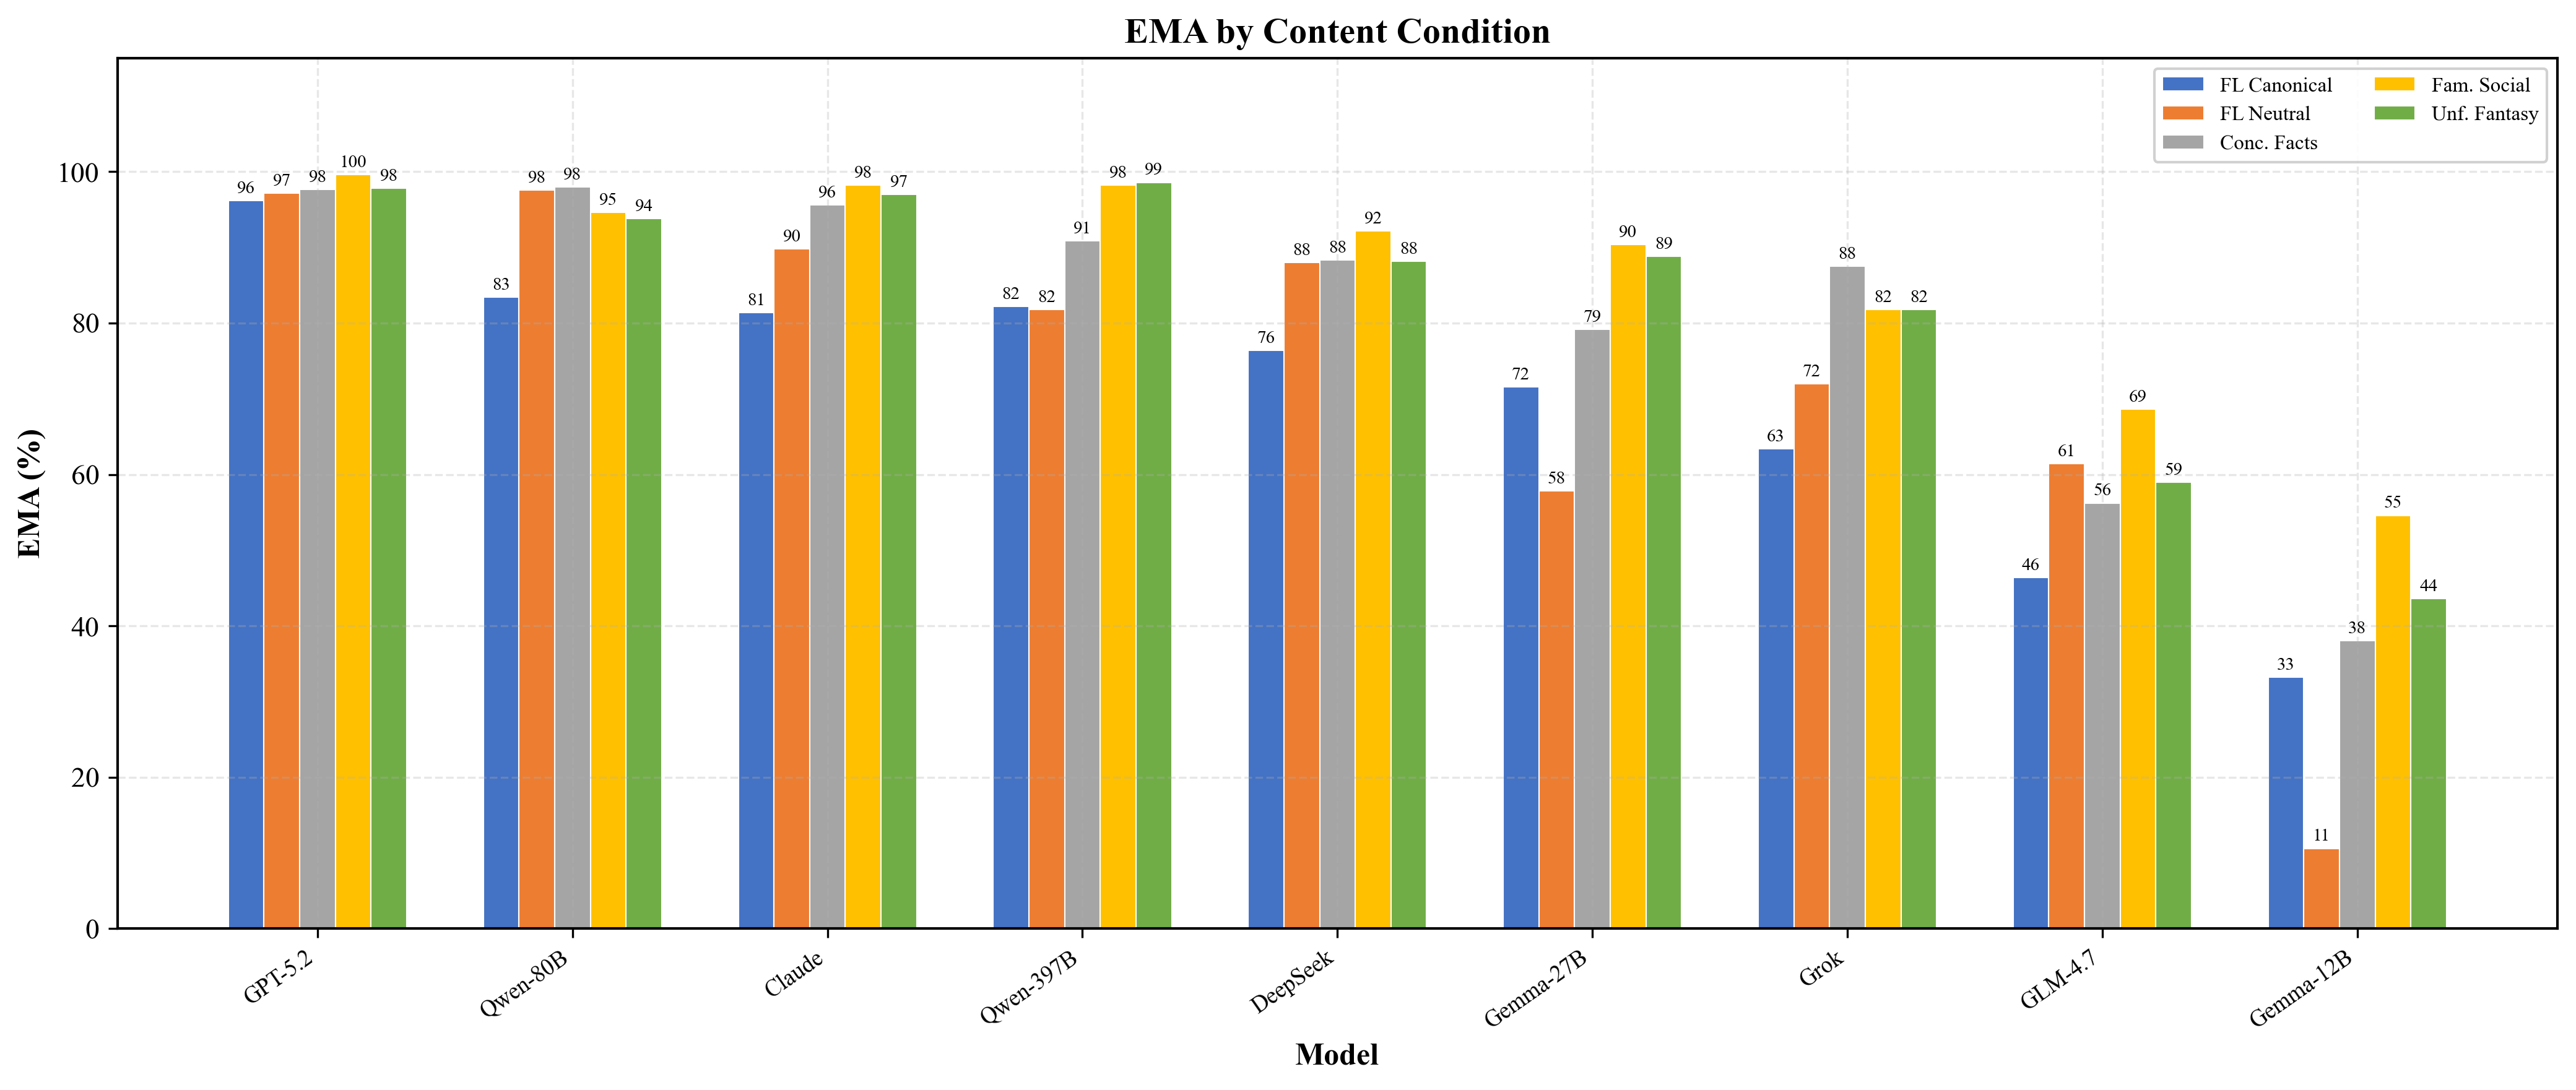
\includegraphics[width=0.95\textwidth]{../experiments_raw_results/wason-selection/figures/wason_ema_conditions.png}
\caption{EMA по пяти контентным условиям для всех девяти моделей. Модели отсортированы по убыванию EMA в FL Neutral. Значения выше 0{,}90 достигаются топовыми моделями во всех условиях, в то время как слабые модели демонстрируют значительный разброс в зависимости от контента.}
\label{fig:ema_conditions}
\end{figure}

\begin{figure}[h!]
\centering
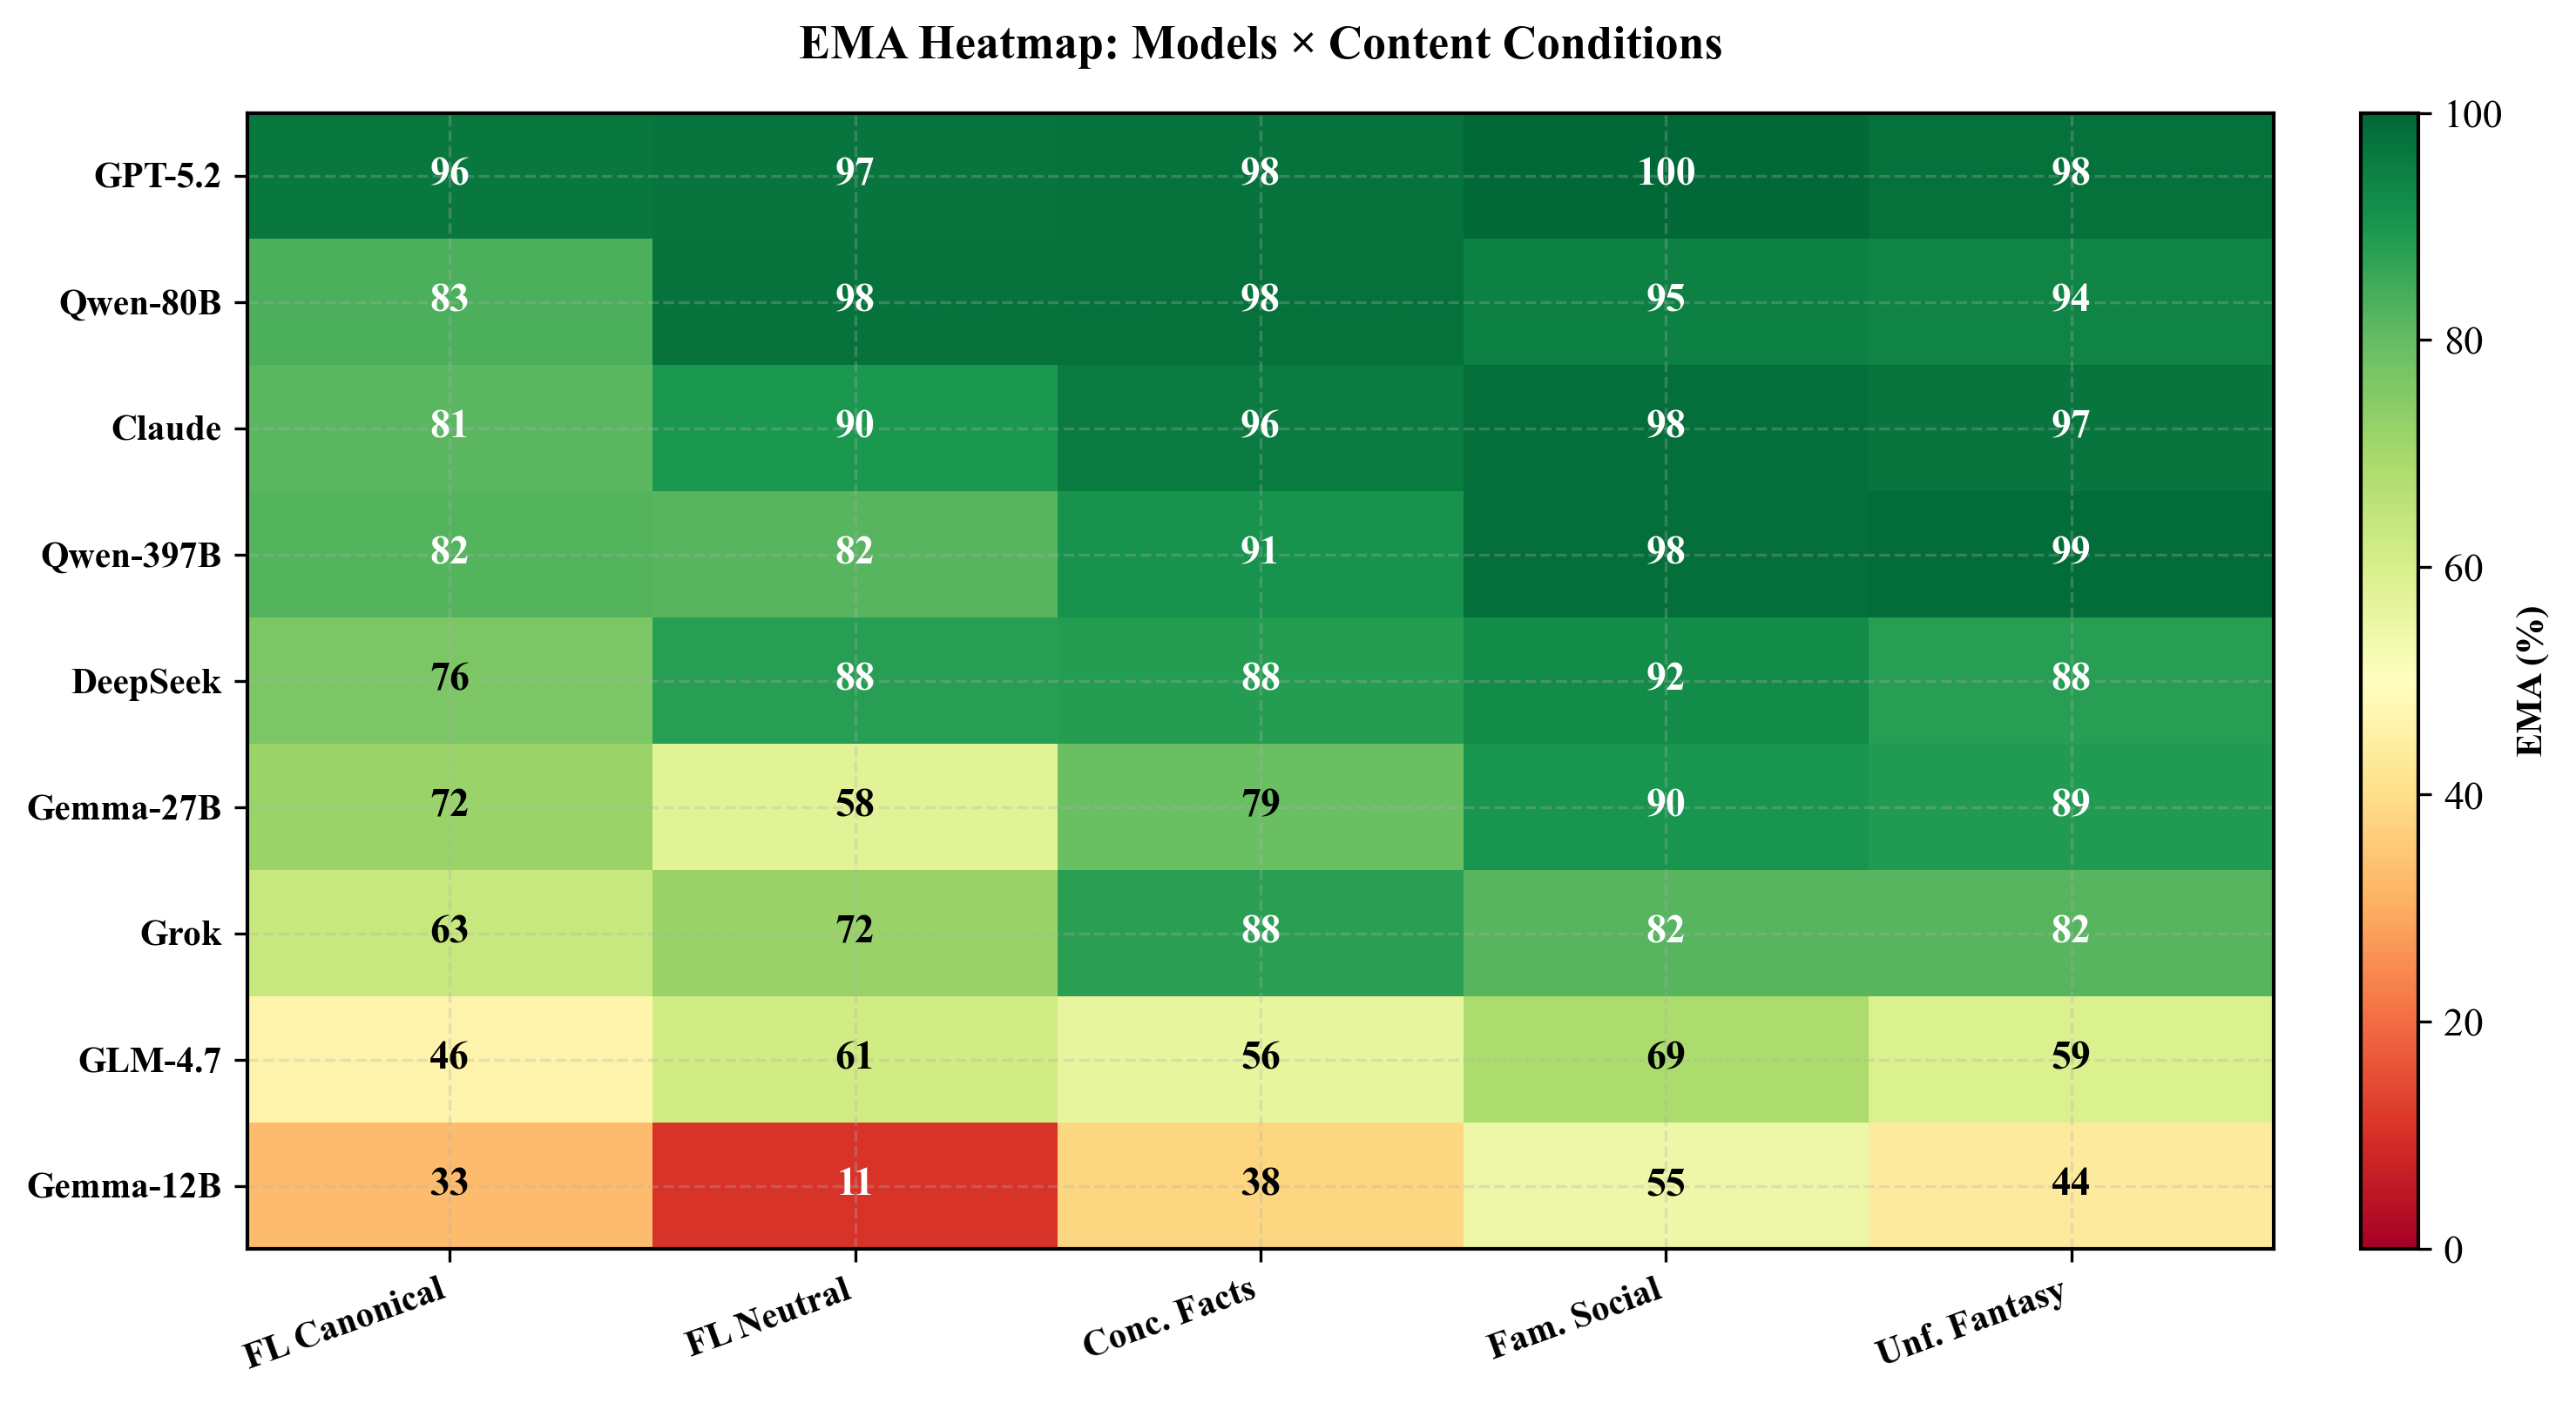
\includegraphics[width=0.95\textwidth]{../experiments_raw_results/wason-selection/figures/wason_ema_heatmap.png}
\caption{Тепловая карта EMA: модели $\times$ контентные условия. Визуализация подчёркивает универсальность контент-эффекта --- все модели без исключения показывают более светлые ячейки в условиях с семантическим содержанием по сравнению с абстрактными.}
\label{fig:ema_heatmap}
\end{figure}

\begin{table}[h!]
\caption{EMA по пяти контентным условиям}
\label{tab:wst_content1}
\centering
\begin{tabular}{|l|c|c|c|c|c|}
\hline
\textbf{Модель} & \textbf{FL Canon.} & \textbf{FL Neutral} & \textbf{Conc. Facts} & \textbf{Fam. Social} & \textbf{Unf. Fantasy} \\
\hline
gpt-5.2                   & 0,973 & 0,972 & 0,976 & 0,996 & 0,978 \\
qwen3-next-80b            & 0,933 & 0,976 & 0,980 & 0,946 & 0,938 \\
qwen3.5-397b-a17b         & 0,867 & 0,818 & 0,909 & 0,982 & 0,986 \\
claude-sonnet-4.6         & 0,907 & 0,898 & 0,956 & 0,982 & 0,970 \\
deepseek-v3.2             & 0,847 & 0,880 & 0,883 & 0,922 & 0,882 \\
grok-4.1-fast             & 0,647 & 0,720 & 0,875 & 0,818 & 0,818 \\
gemma-3-27b-it            & 0,553 & 0,578 & 0,792 & 0,904 & 0,888 \\
glm-4.7-flash             & 0,533 & 0,614 & 0,562 & 0,686 & 0,590 \\
gemma-3-12b-it            & 0,207 & 0,106 & 0,380 & 0,546 & 0,436 \\
\hline
\end{tabular}
\end{table}

\textbf{Контент-эффект} является наиболее устойчивым результатом эксперимента и воспроизводится у всех девяти моделей. Переход от абстрактного нейтрального условия к знакомым социальным контрактам даёт прирост EMA у восьми из девяти моделей (медианный прирост $+0{,}084$): от снижения на $-0{,}030$ у \texttt{qwen3-next-80b} (у которой EMA и так близка к потолку $0{,}976$) до $+0{,}440$ у \texttt{gemma-3-12b-it}. Критически важным является результат условия «Незнакомых фантастических социальных контрактов»: EMA в нём превышает EMA в нейтральном абстрактном условии у семи из девяти моделей (медианный прирост $+0{,}072$) и вплотную приближается к EMA знакомых социальных контрактов. Это поддерживает гипотезу прагматических схем~\cite{cheng1985pragmatic}: деонтическая структура обязательства фасилитирует правильный логический вывод независимо от знакомости содержания.

\begin{figure}[h!]
\centering
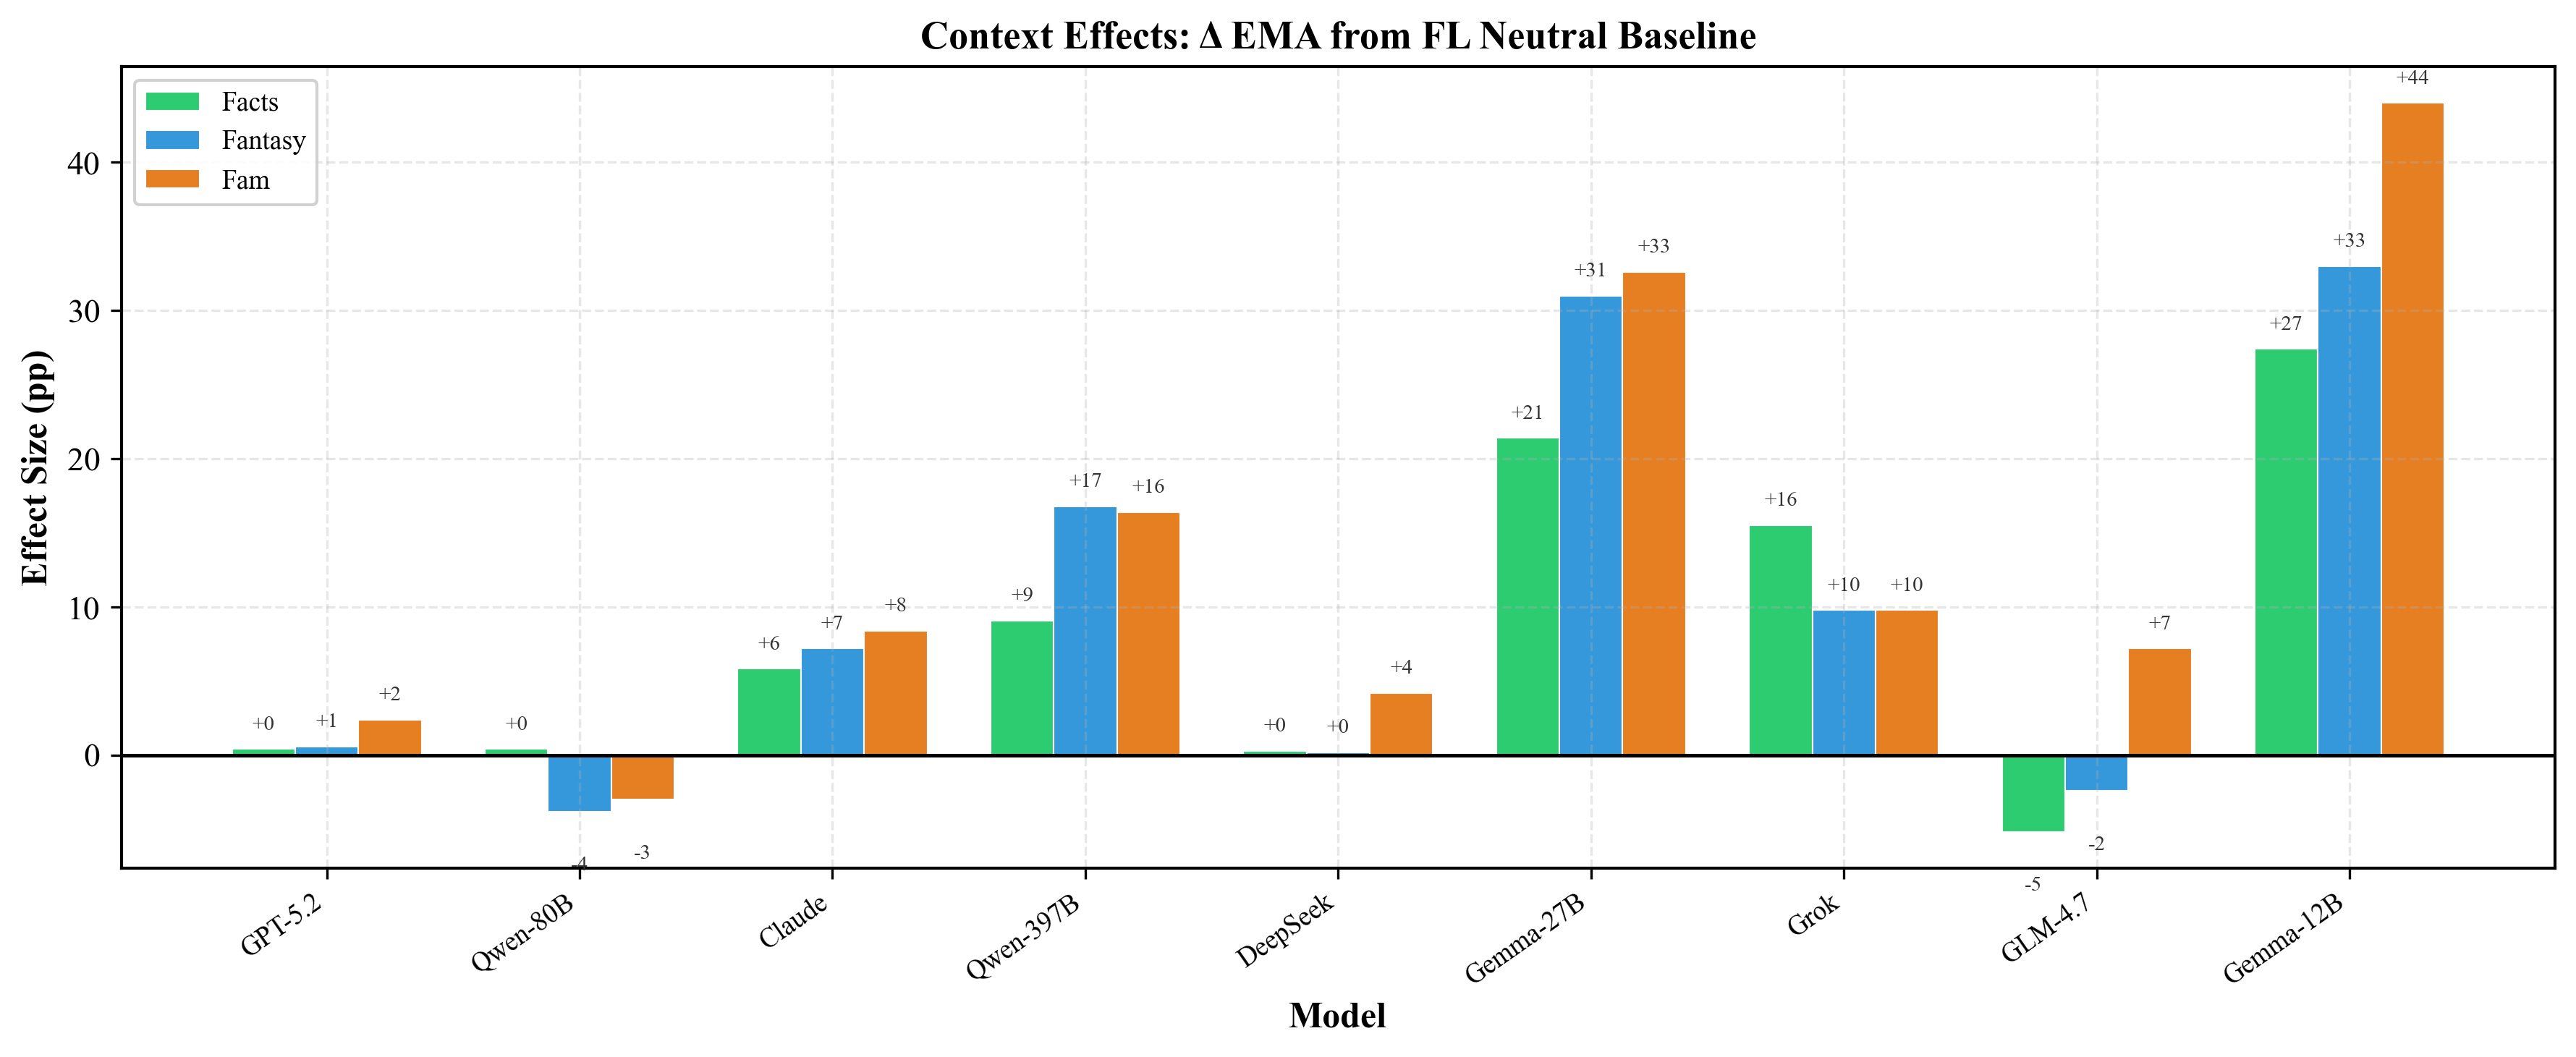
\includegraphics[width=0.85\textwidth]{../experiments_raw_results/wason-selection/figures/wason_context_effects.png}
\caption{Контент-эффект: изменение EMA при переходе от FL Neutral к Familiar Social Contracts (синий) и Unfamiliar Fantasy Social Contracts (оранжевый). Фасилитация наблюдается у всех моделей, причём Fantasy Social условия дают EMA, сопоставимый с Familiar Social, что подтверждает гипотезу деонтической структуры.}
\label{fig:context_effects}
\end{figure}

Исключением является \texttt{gemma-3-27b-it}, у которой EMA в условии Fantasy ($0{,}888$) лишь незначительно уступает Familiar ($0{,}904$), при этом EMA в нейтральном абстрактном условии ($0{,}578$) заметно ниже --- что указывает на особую чувствительность этой модели именно к деонтическому фреймингу, а не к знакомости содержания.

\textbf{Предубеждение подтверждения} подтверждено для всех моделей в нейтральном промпт-условии. В Formal Logic Neutral \texttt{gemma-3-12b-it} демонстрирует совокупный индекс bias (MBI + CBR) $= 0{,}536$ при EMA $= 0{,}106$ --- модель выбирает предубеждённый ответ в 5 раз чаще правильного, причём доминирующей ошибкой является Matching Bias ($0{,}516$). У \texttt{glm-4.7-flash} MBI $= 0{,}190$, CBR $= 0{,}040$ при EMA $= 0{,}614$; у \texttt{gemma-3-27b-it} MBI $= 0{,}296$ при EMA $= 0{,}578$. В контрасте, у моделей-лидеров MBI не превышает $0{,}020$ (кроме \texttt{claude-sonnet-4.6} с MBI $= 0{,}078$), а CBR равен нулю у пяти из девяти моделей. Важно, что контент-эффект снижает bias: переход к Familiar Social уменьшает MBI у \texttt{gemma-3-12b-it} с $0{,}516$ до $0{,}144$, а у \texttt{gemma-3-27b-it} --- с $0{,}296$ до $0{,}086$.

\begin{table}[h!]
\caption{MBI и CBR по пяти контентным условиям}
\label{tab:wst_bias}
\centering
\begin{tabular}{|l|cc|cc|cc|cc|cc|}
\hline
\multirow{2}{*}{\textbf{Модель}} & \multicolumn{2}{c|}{\textbf{FL Canon}} & \multicolumn{2}{c|}{\textbf{FL Neutral}} & \multicolumn{2}{c|}{\textbf{Conc. Facts}} & \multicolumn{2}{c|}{\textbf{Fam. Social}} & \multicolumn{2}{c|}{\textbf{Unf. Fantasy}} \\
\cline{2-11}
 & MBI & CBR & MBI & CBR & MBI & CBR & MBI & CBR & MBI & CBR \\
\hline
gemma-3-12b-it    & 0,493 & 0,020 & 0,516 & 0,020 & 0,285 & 0,018 & 0,144 & 0,000 & 0,236 & 0,004 \\
glm-4.7-flash     & 0,293 & 0,027 & 0,190 & 0,040 & 0,275 & 0,053 & 0,262 & 0,002 & 0,334 & 0,000 \\
gemma-3-27b-it    & 0,267 & 0,000 & 0,296 & 0,000 & 0,182 & 0,000 & 0,086 & 0,000 & 0,102 & 0,002 \\
grok-4.1-fast     & 0,153 & 0,000 & 0,170 & 0,000 & 0,067 & 0,000 & 0,054 & 0,000 & 0,082 & 0,000 \\
claude-sonnet-4.6 & 0,080 & 0,000 & 0,078 & 0,000 & 0,026 & 0,000 & 0,006 & 0,000 & 0,024 & 0,000 \\
deepseek-v3.2     & 0,013 & 0,000 & 0,020 & 0,000 & 0,014 & 0,000 & 0,028 & 0,002 & 0,028 & 0,000 \\
qwen3-next-80b    & 0,060 & 0,000 & 0,014 & 0,000 & 0,006 & 0,000 & 0,032 & 0,000 & 0,030 & 0,000 \\
qwen3.5-397b-a17b & 0,000 & 0,000 & 0,012 & 0,002 & 0,004 & 0,000 & 0,000 & 0,000 & 0,004 & 0,000 \\
gpt-5.2           & 0,000 & 0,000 & 0,000 & 0,004 & 0,004 & 0,000 & 0,002 & 0,000 & 0,010 & 0,000 \\
\hline
\end{tabular}
\end{table}

\textbf{Сравнение с человеческой производительностью.} Результаты LLM интерпретируются относительно эмпирических бейзлайнов людей (таблица~\ref{tab:human_wason}). Таблица~\ref{tab:human_llm_comparison} сопоставляет ключевые метрики.

\begin{table}[h!]
\caption{Сравнение производительности LLM с эмпирическими данными людей в задаче выбора Уэйсона}
\label{tab:human_llm_comparison}
\centering
\begin{tabular}{|l|c|c|c|}
\hline
\textbf{Метрика} & \textbf{Люди (абстрактная)} & \textbf{LLM топ-3} & \textbf{LLM слабые\textsuperscript{*}} \\
\hline
EMA (правильный ответ) & 4--19\% & 90--98\% & 10--61\% \\
Matching bias (P+Q) & 39--45\% & 0--2\% & 19--52\% \\
Confirmation (только P) & 33--36\% & 0\% & 0--4\% \\
Контент-эффект (доступ $\rightarrow$ соц.) & $+45$ п.п. & $+3$--$15$ п.п. & $+9$--$+44$ п.п. \\
\hline
\end{tabular}
\\[2pt]
\raggedright\footnotesize\textsuperscript{*}\texttt{gemma-3-12b-it}, \texttt{glm-4.7-flash}, \texttt{gemma-3-27b-it} --- три модели с наименьшей EMA в FL Neutral.
\end{table}

Даже слабейшая из протестированных моделей (\texttt{gemma-3-12b-it}, EMA~=~10{,}6\%) демонстрирует производительность на уровне нижней границы человеческого диапазона (4--19\%), а топовые модели превосходят людей на порядок. Однако паттерн ошибок у слабых LLM качественно родственен человеческому: доминирующей ошибкой является matching bias ($\{$P, Q$\}$), составляющий 51{,}6\% ответов \texttt{gemma-3-12b-it} --- это превышает верхнюю границу человеческого диапазона (45\%), хотя качественный паттерн доминирования matching bias совпадает.

Контент-эффект воспроизводит человеческий паттерн: и люди, и LLM улучшаются при переходе от абстрактных правил к деонтическим (социальным контрактам). У людей прирост составляет $\approx$+45 процентных пунктов (19\% $\rightarrow$ 64\%); у LLM медианный прирост от FL Neutral к Familiar Social составляет $+0{,}084$ ($+8{,}4$ п.п.), а у наиболее уязвимых моделей --- до $+0{,}440$ у \texttt{gemma-3-12b-it}. Масштаб эффекта у людей больше, что объясняется существенно более низким базисом в абстрактном условии. Направление эффекта --- одинаковое: деонтическая структура фасилитирует нормативное рассуждение у обоих типов агентов.

\begin{table}[h!]
\caption{Сравнение промпт-условий на датасете Formal Logic Neutral}
\label{tab:wst_prompts}
\centering
\begin{tabular}{|l|c|c|c|c|c|c|}
\hline
\multirow{2}{*}{\textbf{Модель}} & \multicolumn{3}{c|}{\textbf{Neutral prompt}} & \multicolumn{3}{c|}{\textbf{CoT prompt}} \\
\cline{2-7}
 & EMA & MBI & CBR & EMA & MBI & CBR \\
\hline
gpt-5.2            & 0,884 & 0,056 & 0,002 & 0,976 & 0,006 & 0,006 \\
claude-sonnet-4.6  & 0,790 & 0,172 & 0,002 & 0,970 & 0,000 & 0,000 \\
qwen3-next-80b     & 0,772 & 0,038 & 0,024 & 0,880 & 0,000 & 0,004 \\
qwen3.5-397b-a17b  & 0,764 & 0,032 & 0,000 & 0,974 & 0,000 & 0,004 \\
deepseek-v3.2      & 0,658 & 0,200 & 0,002 & 0,936 & 0,000 & 0,002 \\
grok-4.1-fast      & 0,424 & 0,450 & 0,000 & 0,664 & 0,032 & 0,252 \\
gemma-3-27b-it     & 0,406 & 0,386 & 0,006 & 0,368 & 0,436 & 0,120 \\
glm-4.7-flash      & 0,332 & 0,304 & 0,248 & 0,258 & 0,086 & 0,548 \\
gemma-3-12b-it     & 0,028 & 0,270 & 0,134 & 0,186 & 0,468 & 0,230 \\
\hline
\end{tabular}
\end{table}

\textbf{Эффект CoT-промпта} является одним из наиболее содержательных результатов. КоТ-промт оценивался на тех же 500 испытаниях (100 правил $\times$ 5 перестановок) в условии FL Neutral для открытых и проприетарных моделей. Полный CoT delta представлен на рисунке~\ref{fig:cot_delta}.

\begin{figure}[h!]
\centering
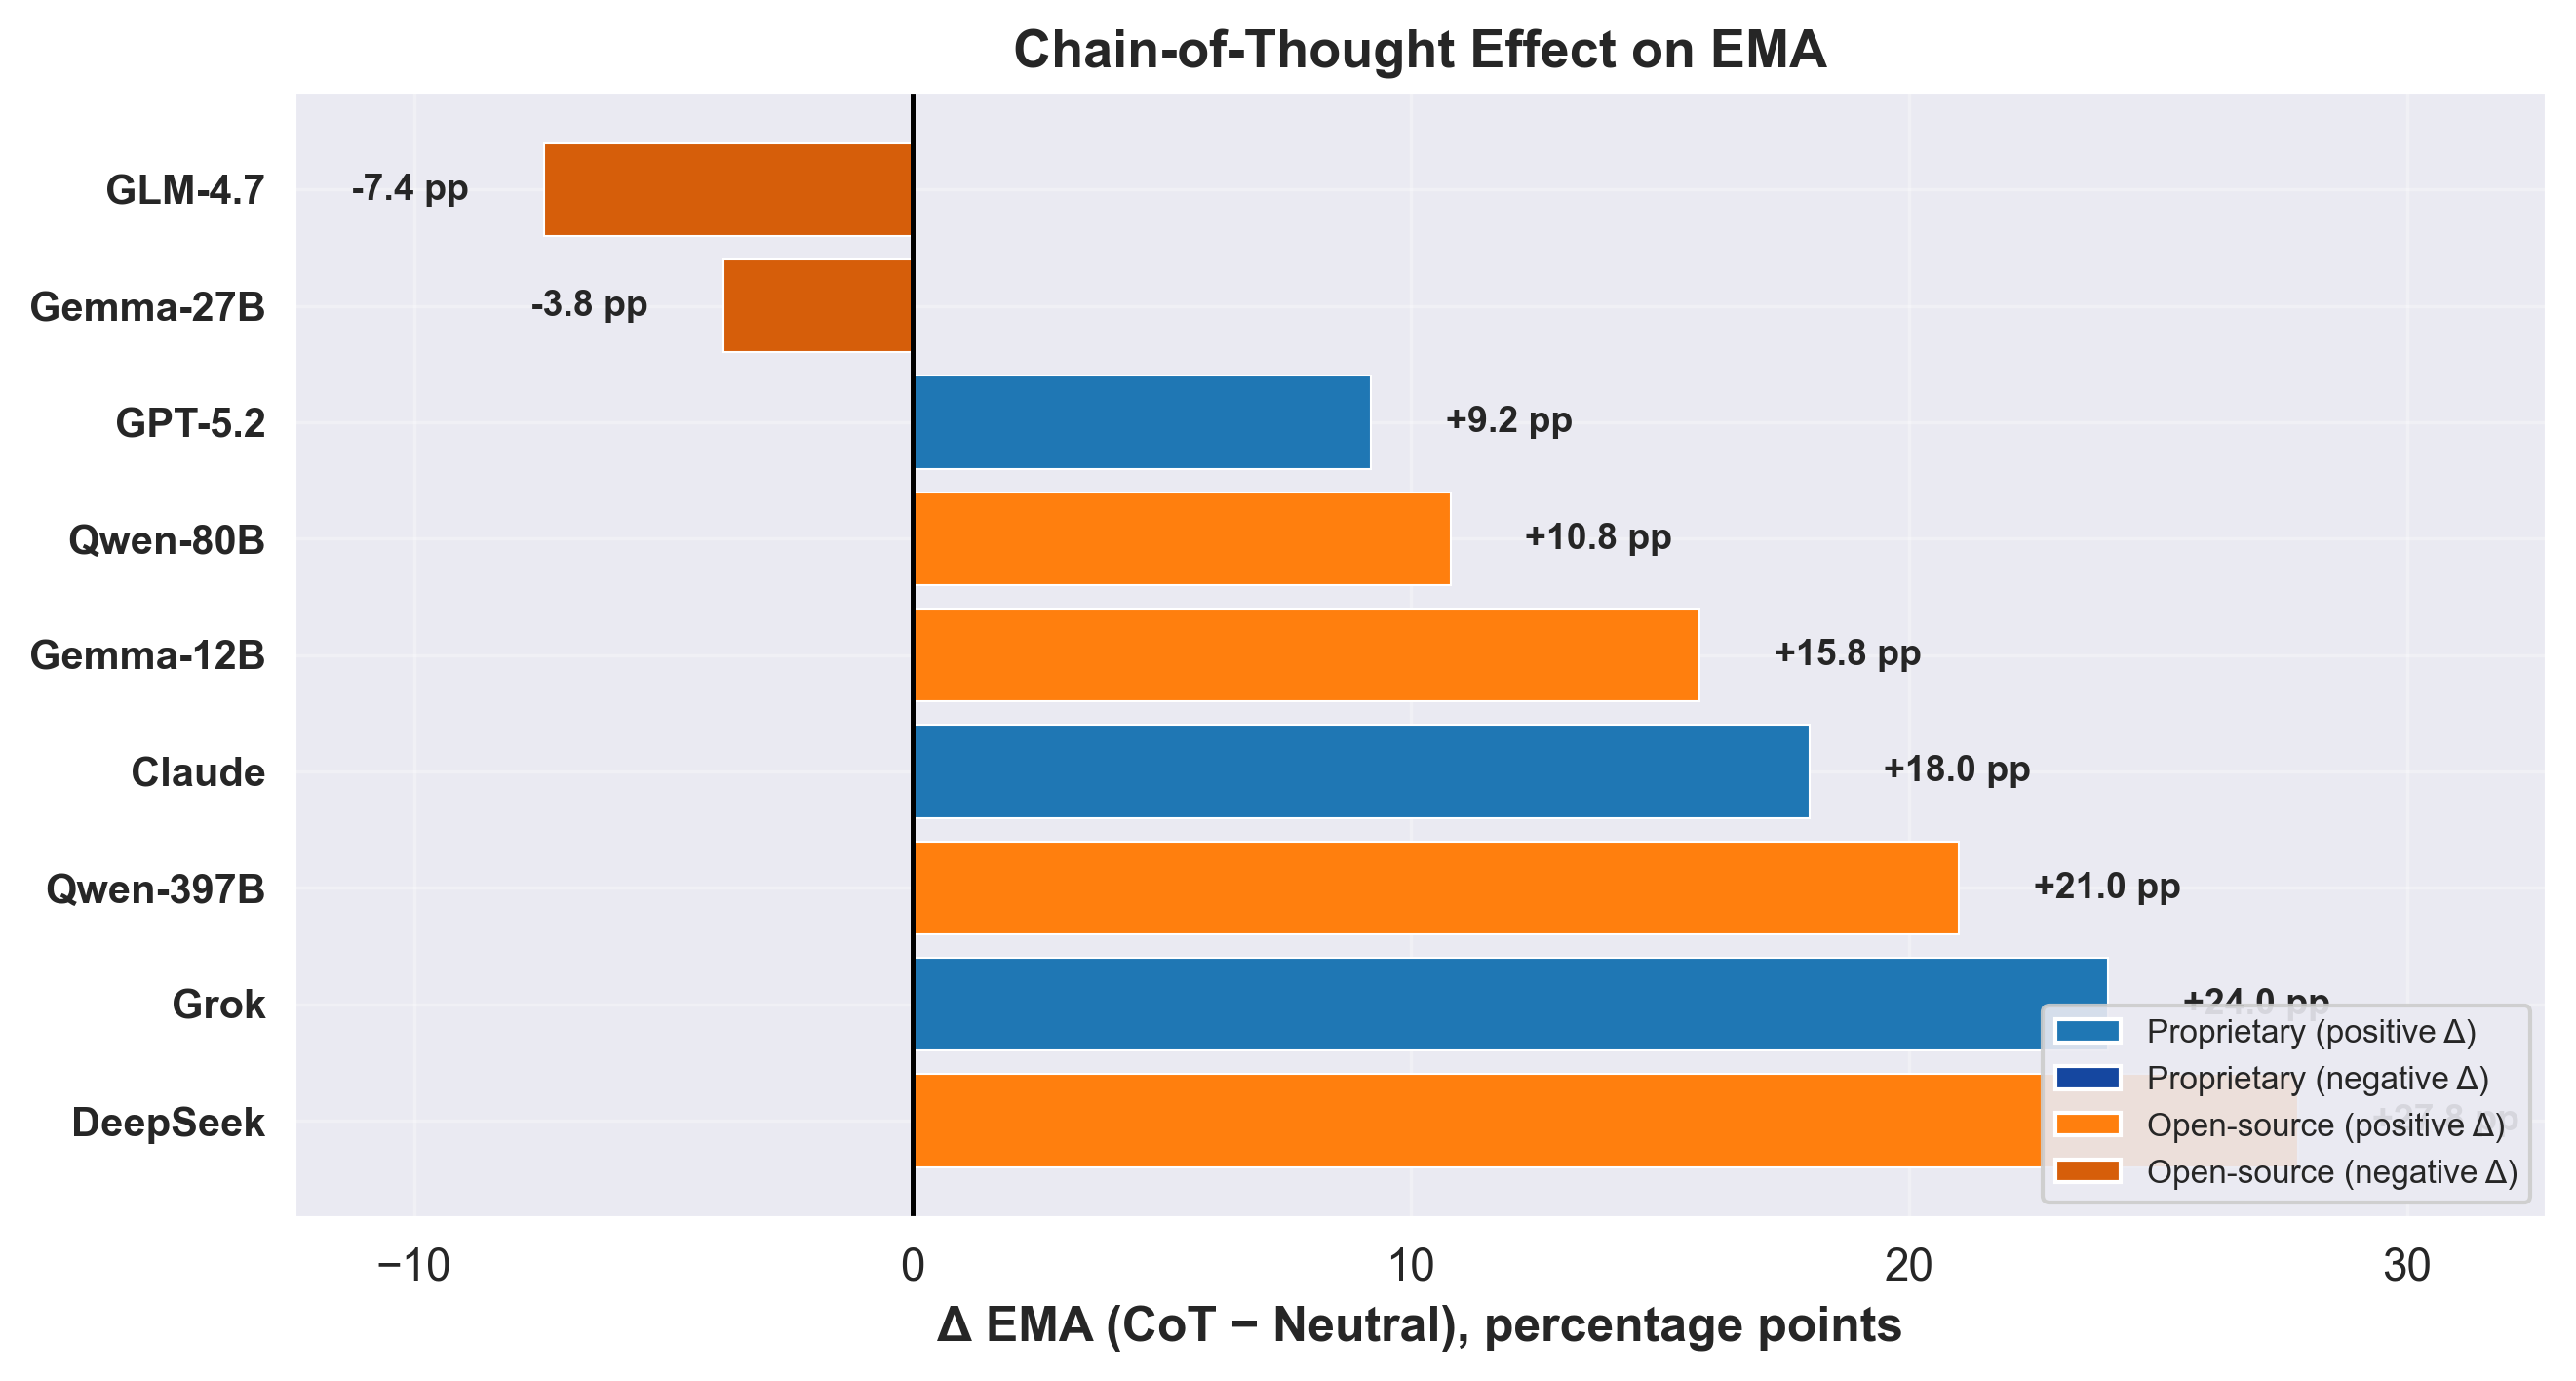
\includegraphics[width=0.85\textwidth]{../experiments_raw_results/wason-selection/output/thesis_graphs/wason_cot_delta.png}
\caption{CoT delta: изменение EMA при переходе от Neutral к CoT промпту. Для проприетарных моделей (синий) CoT даёт прирост у всех трёх моделей. Для открытых моделей (оранжевый) две модели демонстрируют отрицательный delta. Модели отсортированы по убыванию delta.}
\label{fig:cot_delta}
\end{figure}

Для проприетарных моделей CoT даёт положительный эффект у всех трёх: \texttt{grok-4.1-fast} (+0,240), \texttt{claude-sonnet-4.6} (+0,180), \texttt{gpt-5.2} (+0,092). При этом MBI и CBR у \texttt{claude} и \texttt{gpt-5.2} падают до нуля --- CoT не только повышает правильность, но и устраняет систематические ошибки.

Для открытых моделей картина дифференцирована. Четыре из шести показывают положительный delta: \texttt{deepseek-v3.2} (+0,278), \texttt{qwen3.5-397b-a17b} (+0,210), \texttt{gemma-3-12b-it} (+0,158), \texttt{qwen3-next-80b} (+0,108). Однако у \texttt{glm-4.7-flash} EMA снижается с 0,332 до 0,258 ($\Delta = -0{,}074$), а CBR вырастает с 0,248 до 0,548: явное рассуждение систематически приводит эту модель к выбору только карточки $\{$P$\}$ --- чистому confirmation bias. У \texttt{gemma-3-27b-it} CoT не меняет EMA содержательно (0,406 vs 0,368, $\Delta = -0{,}038$), однако перераспределяет ошибки: MBI растёт с 0,386 до 0,436, то есть явное рассуждение усиливает предубеждение соответствия. Это указывает на то, что CoT не является универсальным средством коррекции предубеждений и может давать обратный эффект у моделей с недостаточной базовой логической компетентностью~\cite{kojima2022large}.

\textbf{Стабильность ответов} в Formal Logic Neutral при нейтральном промпте варьирует от 0,110 у \texttt{gemma-3-12b-it} до 0,910 у \texttt{qwen3-next-80b}. Примечательно, что \texttt{qwen3-next-80b} демонстрирует наивысшую стабильность (0,910) при EMA 0,976 --- сочетание, нетипичное для других моделей. \texttt{gemma-3-27b-it} при EMA 0,578 имеет стабильность лишь 0,280 --- низкую относительно точности, что указывает на нестабильное угадывание, а не на систематическое рассуждение.

\begin{figure}[h!]
\centering
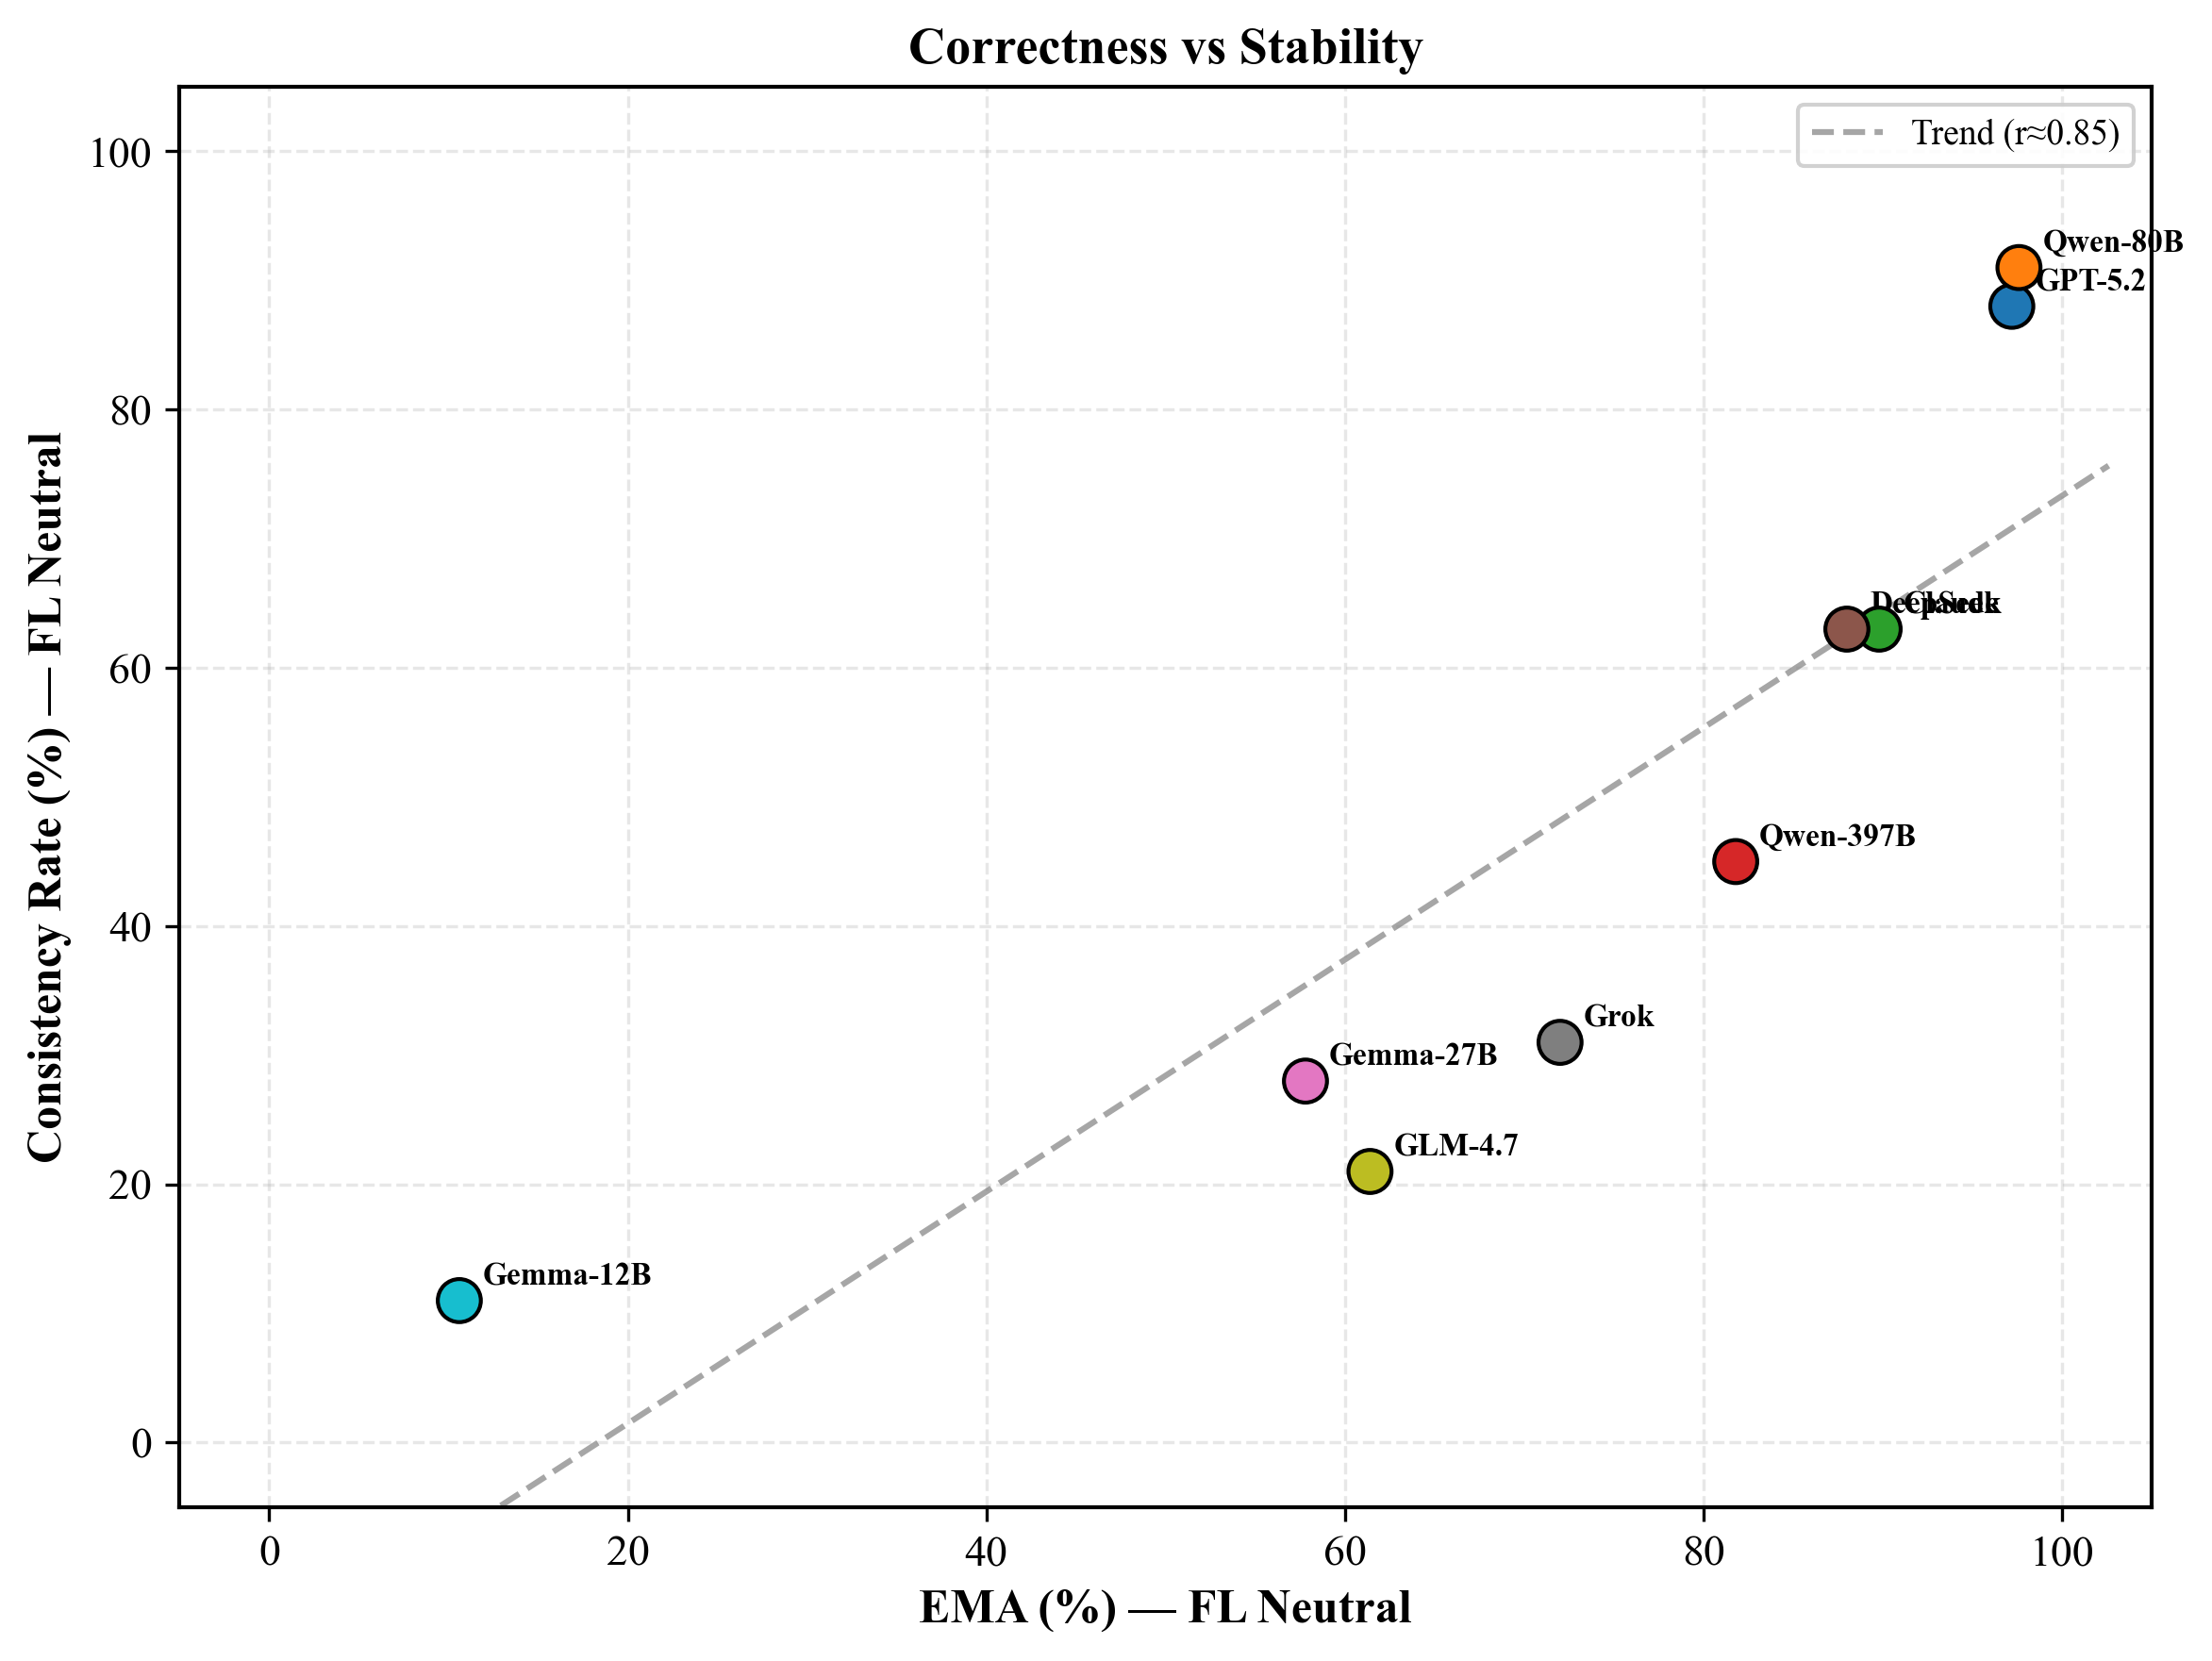
\includegraphics[width=0.85\textwidth]{../experiments_raw_results/wason-selection/figures/wason_ema_vs_consistency.png}
\caption{Связь EMA и Consistency Rate в FL Neutral. Идеальная модель находилась бы в правом верхнем углу (высокая точность + высокая стабильность). Топ-модели кластеризуются вблизи этого угла, в то время как слабые модели демонстрируют различные профили: низкая точность + низкая стабильность (\texttt{gemma-3-12b-it}), средняя точность + низкая стабильность (\texttt{gemma-3-27b-it}).}
\label{fig:ema_vs_consistency}
\end{figure}

\textbf{Внутрисемейный парадокс.} В семействе Gemma эффект из эксперимента 1 инвертируется: по EMA в Formal Logic Neutral \texttt{gemma-3-27b-it} ($0{,}578$) значительно превосходит \texttt{gemma-3-12b-it} ($0{,}106$). Таким образом, в вероятностной задаче 27b была более уязвима, чем 12b, а в логической задаче --- менее уязвима. Это указывает на то, что уязвимость к разным типам когнитивных предубеждений не определяется единым фактором и может иметь различную направленность в зависимости от типа рассуждения.

\subsection{Качественный анализ категорий ошибок}

Помимо агрегированных метрик, классификация ответов на шесть содержательных категорий позволяет детально описать паттерны ошибочного рассуждения. Ниже приведены категории, их частоты в FL Neutral (наиболее «чистом» условии) и типичные примеры.

\textbf{1. CORRECT} ($\{$P, $\lnot$Q$\}$). Нормативно правильный ответ. В FL Neutral варьирует от 10,6\% (\texttt{gemma-3-12b-it}) до 97,6\% (\texttt{qwen3-next-80b}).

\textbf{2. MATCHING BIAS} ($\{$P, Q$\}$). Выбор обеих карточек, явно упомянутых в правиле. Каноническая ошибка, описанная ещё у Evans~\cite{evans1998matching}. Доминирующая ошибка слабых моделей: \texttt{gemma-3-12b-it} допускает её в 51,6\% испытаний.

\begin{quote}
\textit{Правило:} «If there is an A on one side, then there is a 3 on the other side.»\\
\textit{Ответ gemma-3-12b-it:} \texttt{['A', '3']} — выбрала именно те карточки, что названы в правиле (P + Q).
\end{quote}

\textbf{3. CONFIRMATION BIAS} ($\{$P$\}$). Выбор только подтверждающей карточки, без проверки $\lnot$Q. Относительно редкая категория (0--4\% у большинства моделей), но существенная у \texttt{gemma-3-12b-it} (2,0\%) и \texttt{glm-4.7-flash} (4,0\%).

\begin{quote}
\textit{Правило:} «If there is a U on the card, then there is an 8 on the back.»\\
\textit{Ответ gemma-3-12b-it:} \texttt{['U']} --- единственная P, игнорирует необходимость проверки $\lnot$Q.
\end{quote}

\textbf{4. LOGIC ERROR} (другие неправильные комбинации). Включает выбор $\{$not\_P, not\_Q$\}$, $\{$not\_P, Q$\}$, одиночных $\{$Q$\}$ или $\{$not\_Q$\}$ и другие неклассифицируемые ответы. Вторая по частоте ошибка после matching bias.

\begin{quote}
\textit{Правило:} «If the number is 6, then the letter is S.»\\
\textit{Ответ gemma-3-12b-it:} \texttt{['9', 'P']} — выбрала not\_P + not\_Q, что является полной инверсией логики.
\end{quote}

\textbf{5. OVER-SELECTION} (более 2 карточек, но не все 4). Редкая категория (0,4--2,2\%), встречается преимущественно у слабых моделей при деонтическом контенте.

\begin{quote}
\textit{Правило:} «If the element is Gold, then it does not Rust.»\\
\textit{Ответ glm-4.7-flash:} \texttt{['Gold', 'Does not rust', 'Iron']} --- 3 карточки, попытка «перестраховаться».
\end{quote}

\textbf{6. ALL CARDS} (все 4 карточки). Крайняя форма неопределённости: модель выбирает все доступные карточки. Встречается в 0,2--1,1\% испытаний.

\begin{quote}
\textit{Правило:} «If the animal is a Camel, then it has a Hump.»\\
\textit{Ответ gemma-3-12b-it:} \texttt{['Camel', 'Hump', 'Horse', 'No hump']} --- все 4 карточки.
\end{quote}

Совокупное распределение категорий в FL Neutral отражает иерархию компетентности: у \texttt{gemma-3-12b-it} 51,6\% Matching Bias + 11,1\% Logic Error + 2,0\% Confirmation Bias = 64,7\% ошибок трёх главных типов, в то время как у \texttt{gpt-5.2} 0,0\% + 2,4\% + 0,4\% = 2,8\%.

\subsection{Выводы по эксперименту 2}

Эксперимент 2 установил:

\begin{enumerate}
  \item \textbf{Предубеждение подтверждения} в дедуктивном рассуждении у всех девяти моделей в нейтральном условии. Совокупный индекс bias (MBI + CBR) варьирует от 0,4\% у \texttt{gpt-5.2} до 53,6\% у \texttt{gemma-3-12b-it}, причём доминирующей ошибкой является matching bias, а не confirmation bias в строгом смысле.

  \item \textbf{Устойчивый контент-эффект} --- социальные контракты решаются значимо лучше абстрактных правил у 8 из 9 моделей (медианный прирост EMA $+0{,}084$). Переход к Familiar Social одновременно снижает MBI: у \texttt{gemma-3-12b-it} с $0{,}516$ до $0{,}144$.

  \item \textbf{Поддержка гипотезы прагматических схем} Ченга-Холиоака через условие фантастических социальных контрактов, которое даёт EMA, сопоставимое со знакомыми контрактами (медианный прирост от FL Neutral $+0{,}072$). Деонтическая структура обязательства фасилитирует логический вывод независимо от знакомости содержания.

  \item \textbf{Дифференцированный эффект CoT} --- проприетарные модели все улучшаются (median $\Delta = +0{,}180$), тогда как 2 из 6 открытых моделей показывают отрицательный delta: \texttt{glm-4.7-flash} ($-0{,}074$) и \texttt{gemma-3-27b-it} ($-0{,}038$). CoT не является универсальной коррекцией предубеждений.

  \item \textbf{Инверсия внутрисемейного парадокса Gemma} по сравнению с экспериментом 1: 27b превосходит 12b в логической задаче, но была более уязвима в вероятностной, что свидетельствует о мультидимензиональности когнитивных предубеждений.

  \item \textbf{Шесть качественных категорий ошибок}, из которых matching bias доминирует у слабых моделей (до 51,6\%), в то время как confirmation bias в строгом смысле (выбор только P) составляет 0--4\% у большинства моделей.

  \item \textbf{Сравнение с человеческой производительностью.} Топовые модели превосходят людей на порядок по EMA (90--98\% vs 4--19\%), однако слабые модели воспроизводят качественно аналогичный паттерн ошибок: доминирование matching bias, низкий уровень строгого confirmation bias, а также положительный контент-эффект при деонтическом framing. Направление контент-эффекта совпадает у людей и LLM, но масштаб различается из-за разного базиса в абстрактном условии.
\end{enumerate}


% -------------------------------------------------------
\section{Эксперимент 3: Задача открытия правила 2-4-6}
% -------------------------------------------------------

\subsection{Обоснование выбора парадигмы}

Задача открытия правила 2-4-6, введённая Уэйсоном~\cite{wason1960failure}, является классической парадигмой для исследования предубеждения подтверждения в индуктивном рассуждении. В оригинальном эксперименте испытуемым сообщалось, что тройка $(2, 4, 6)$ удовлетворяет скрытому правилу, и предлагалось открыть его, предлагая новые тройки и получая бинарную обратную связь. Канонический результат: испытуемые тестируют тройки, согласующиеся с текущей гипотезой (например, $(4, 8, 10)$ для гипотезы «чётные числа в порядке возрастания»), вместо попыток фальсифицировать её, и не обнаруживают истинное правило («любая возрастающая последовательность»).

В отличие от экспериментов 1 и 2, где предубеждение проявляется в единственном ответе, здесь оно измеряется как свойство \textit{стратегии} на протяжении многоходового диалога.

\subsection{Конструкция датасета правил: пять таксономических категорий}

Был сформирован независимый датасет из \textbf{50 правил}, организованных в пять таксономических категорий:

\begin{itemize}
  \item \textbf{Порядок и сравнение} (9 правил) --- отношения между элементами: $x < y < z$, $x > y \land z > y$;
  \item \textbf{Чётность и делимость} (10 правил) --- свойства модульной арифметики: все чётные, сумма кратна 3;
  \item \textbf{Арифметические отношения} (10 правил) --- аддитивные и мультипликативные структуры: $x + y = z$, $y - x = z - y$;
  \item \textbf{Структурные паттерны} (11 правил) --- позиционные и теоретико-множественные свойства: $\max(x, y, z) = z$, ровно два уникальных значения;
  \item \textbf{Смешанные / составные} (10 правил) --- конъюнкции из предыдущих категорий: $x < y < z \land (x + y + z) \equiv 0 \pmod{2}$.
\end{itemize}

Все правила верифицированы на исполнимость в диапазоне $[1, 99]^3$, отсутствие функциональных дубликатов (проверка через экстенсиональную эквивалентность) и отсутствие тавтологий. Ряд правил намеренно сконструирован как \textit{ловушки специфичности}: правила, являющиеся строго более специфичными, чем истинное правило, но согласующиеся с порождающей тройкой $(2, 4, 6)$. Из 50 правил \textbf{26 удовлетворяются} тройкой $(2, 4, 6)$ и 24 не удовлетворяются.

\subsection{Многоходовой диалоговый протокол}

Эксперимент реализован как многоходовой диалог. На каждом ходу $t$ модель получает историю разговора и должна ответить в строго ограниченном формате:

\begin{quote}
\texttt{H: lambda x, y, z: <hypothesis>}\\
\texttt{T: [x, y, z]}
\end{quote}

где \texttt{H} --- исполняемый Python-лямбда-выражение, представляющее текущую гипотезу о скрытом правиле $R$, а \texttt{T} --- следующая тройка для тестирования. Модель получает только бинарную обратную связь вида \texttt{(a, b, c) -> True} или \texttt{(a, b, c) -> False}. Испытание завершается либо по достижении \texttt{max\_turns}, либо при выполнении условия ранней остановки: $\text{IOU}(H_t, R) > 0{,}95$ на текущей Монте-Карло выборке~--- в зависимости от того, что наступит раньше. Это объясняет, почему среднее число ходов у reasoning-модели (\texttt{mean\_turns} $\approx 15$) меньше \texttt{max\_turns}: часть траекторий завершается досрочно при успешном обнаружении правила. В отличие от бенчмарка WILT~\cite{banatt2024wilt}, дизайн настоящего исследования требует от модели поддерживать живую, исполняемую гипотезу \textit{на каждом ходу}, что позволяет анализировать полную траекторию гипотез.

\subsection{Промпт-условия: Baseline и Adaptive}

Оба условия используют одинаковую структуру диалога: стартовое сообщение пользователя содержит только \texttt{True} (подтверждение того, что тройка $(2, 4, 6)$ удовлетворяет правилу), на каждом последующем ходу модель получает бинарную обратную связь вида \texttt{(x, y, z) -> True} или \texttt{(x, y, z) -> False}. Ответ модели должен быть оформлен в блоке \texttt{```python```} и содержать ровно две строки: гипотезу \texttt{H} и тестируемую тройку \texttt{T}.

\textbf{Baseline.} Системный промпт содержит фрейм задачи, требуемый формат и жёсткие технические ограничения без каких-либо метакогнитивных советов:

\begin{quote}
\textit{You have a hidden rule for number triples (x,y,z). The triple (2,4,6) satisfies this rule. Your goal: discover the rule through testing. YOU MUST respond in a fenced python block on EVERY turn [...] Use ONLY positive integers from 1 to 1000 [...] NO explanations, commentary, or reasoning in your response. NO stopping until maximum turns reached.}
\end{quote}

\textbf{Adaptive.} Идентичен baseline по техническим ограничениям и формату, однако дополнен блоком явных метакогнитивных указаний по стратегии тестирования:

\begin{quote}
\textit{CRITICAL TESTING APPROACH: If you get a False result, your hypothesis MUST change to exclude that case. If you get an unexpected True, your hypothesis MUST expand to include it. Prefer tests that could prove your current hypothesis wrong, not just confirm it. Repeatedly proposing triples your current hypothesis already expects to be True is weak testing. Use boundary cases and contrastive cases that distinguish your current hypothesis from nearby alternatives. Consider mathematical properties: sums, products, differences, divisibility, remainders.}
\end{quote}

Манипуляция мотивирована данными Batista и Griffiths~\cite{batista2026rational} о том, что явные инструкции по обратной связи модулируют поведение пересмотра гипотез. Оба условия разделяют требование продолжать тестирование до достижения \texttt{max\_turns} вне зависимости от уверенности модели.

\subsection{Метрики качества гипотез}

\textbf{Ключевой методологической особенностью} является использование \textit{экстенсиональной эквивалентности} для оценки гипотез. Вместо текстового сравнения строк гипотезы оцениваются как множества принятых троек над большой случайной выборкой~\cite{banatt2024wilt}. Формально: для скрытого правила $R$ и гипотезы модели $H_t$ на ходу $t$ сэмплируются $N = 200{,}000$ случайных троек $(x, y, z) \in [1, 99]^3$ и вычисляются булевы векторы $\mathbf{r}$ и $\mathbf{h}_t$. Метрика:
\begin{equation}
  \text{IOU}(H_t, R) = \frac{|\mathbf{h}_t \cap \mathbf{r}|}{|\mathbf{h}_t \cup \mathbf{r}|},
  \label{eq:iou}
\end{equation}
испытание считается \textbf{успешным} при $\text{IOU}(H_T, R) > 0{,}95$.

\textbf{Success Rate} ($\uparrow$) --- доля правил, для которых финальная гипотеза достигает $\text{IOU} > 0{,}95$.

\textbf{Mean AUC-IOU} ($\uparrow$) --- площадь под кривой IOU по ходам, усреднённая по всем правилам:
\begin{equation}
  \text{AUC-IOU} = \frac{1}{T} \sum_{t=1}^{T} \text{IOU}(H_t, R).
  \label{eq:auc_iou}
\end{equation}

\textbf{Confirming Test Rate (CTR)} ($\downarrow$) --- доля ходов, на которых предлагаемая тройка $T_t$ предсказывается текущей гипотезой $H_t$ как True:
\begin{equation}
  \text{CTR} = \frac{1}{T} \sum_{t=1}^{T} \mathbf{1}[H_t(T_t) = \text{True}].
  \label{eq:ctr}
\end{equation}
Напрямую операционализирует предубеждение подтверждения: низкий CTR соответствует фальсификационно-ориентированной стратегии.

\textbf{Hypothesis Change Rate (HCR)} ($\uparrow$) --- доля последовательных пар ходов, на которых модель существенно пересматривает гипотезу:
\begin{equation}
  \text{HCR} = \frac{1}{T-1} \sum_{t=2}^{T} \mathbf{1}[\text{IOU}(H_t, H_{t-1}) < 0{,}9].
  \label{eq:hcr}
\end{equation}
Низкий HCR указывает на «залипание» в начальной гипотезе вне зависимости от полученной обратной связи.

\subsection{Результаты и анализ}

Полные результаты по baseline- и adaptive-условиям представлены в таблице~\ref{tab:246_results}.

\begin{table}[h!]
\caption{Результаты эксперимента 3: baseline и adaptive условия}
\label{tab:246_results}
\centering
\begin{tabular}{|l|c|c|c|c|}
\hline
\textbf{Модель} & \textbf{SR base} & \textbf{SR adap} & \textbf{CTR base} & \textbf{CTR adap} \\
\hline
claude-sonnet-4.6  & 0,28 & 0,28 & 0,812 & 0,787 \\
qwen3.5-397b-a17b  & 0,22 & 0,18 & 0,850 & 0,602 \\
qwen3-next-80b     & 0,20 & 0,24 & 0,976 & 0,719 \\
gpt-5.2            & 0,18 & 0,18 & 0,719 & 0,584 \\
grok-4.1-fast      & 0,14 & 0,08 & 0,629 & 0,672 \\
deepseek-v3.2      & 0,10 & 0,16 & 0,879 & 0,768 \\
gemma-3-12b-it     & 0,06 & 0,04 & 0,747 & 0,718 \\
glm-4.7-flash      & 0,04 & 0,06 & 0,739 & 0,486 \\
gemma-3-27b-it     & 0,04 & 0,10 & 0,688 & 0,842 \\
\hline
claude-sonnet-4.6 reasoning & 0,28 & 0,32 & 0,771 & 0,781 \\
gpt-5.2 reasoning  & 0,38 & 0,48 & 0,726 & 0,559 \\
\hline
\end{tabular}
\end{table}

\begin{figure}[ht]
    \centering
    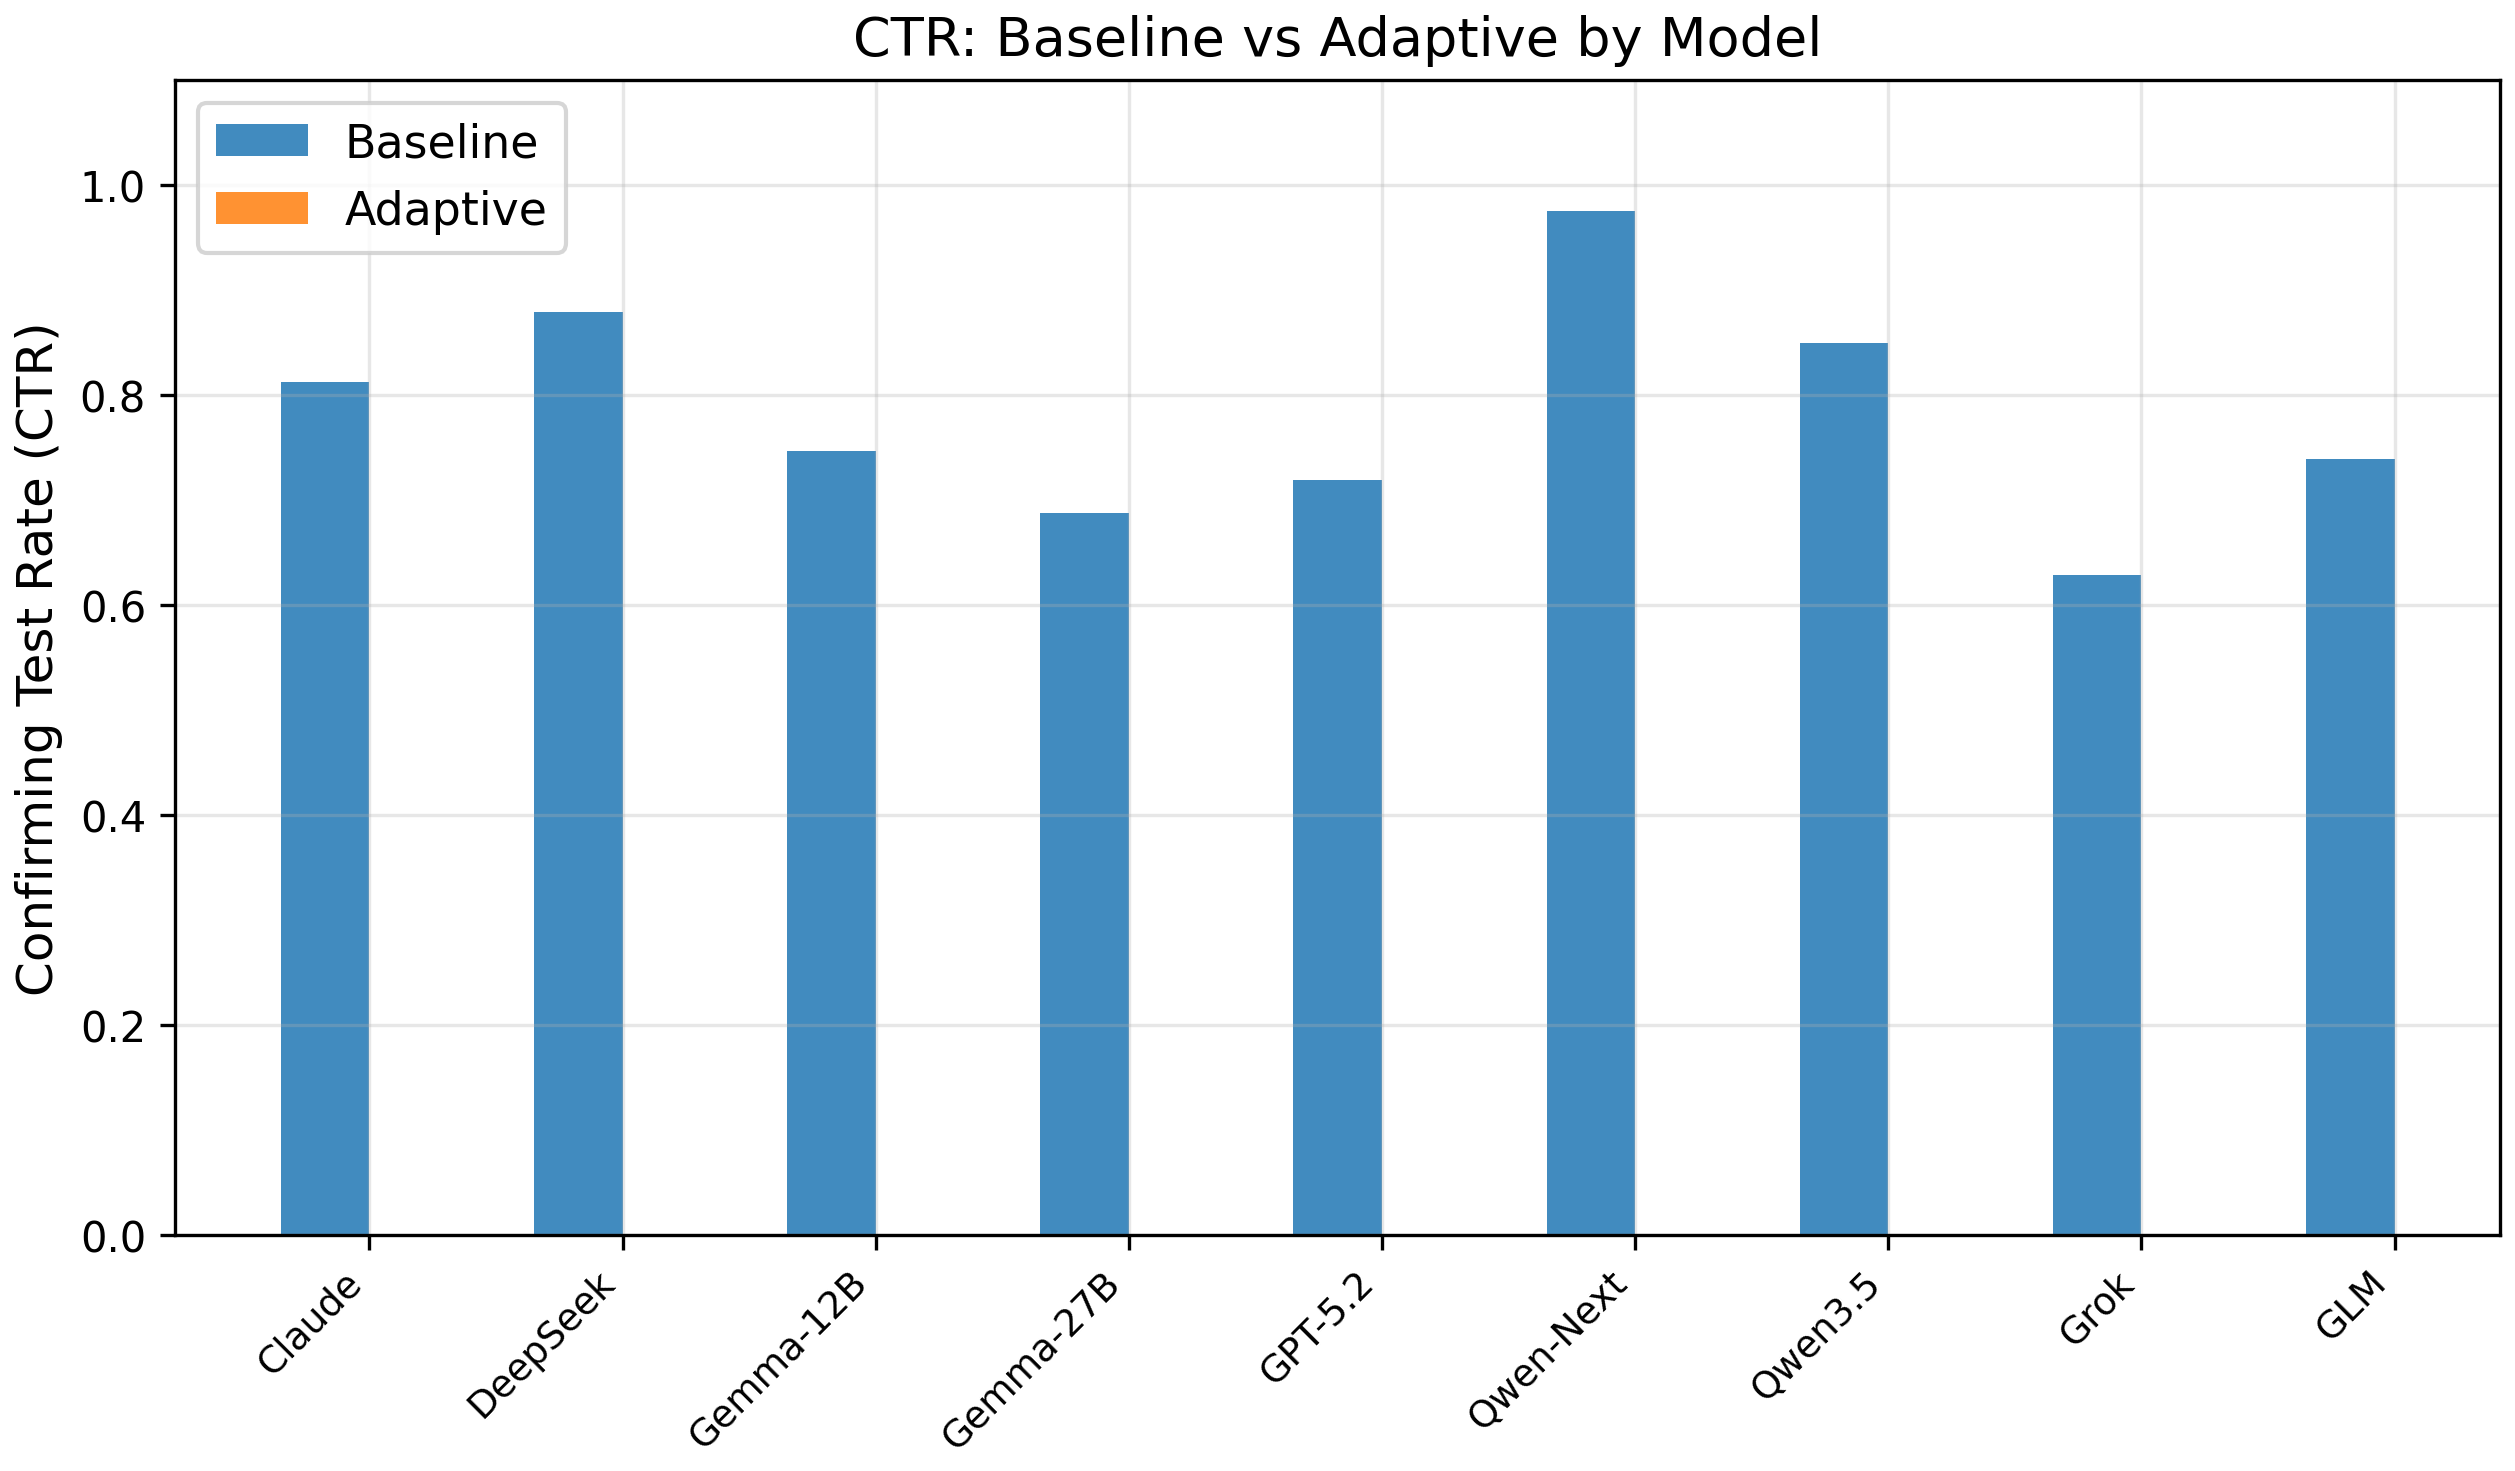
\includegraphics[width=0.8\textwidth]{../experiments_raw_results/wason-2-4-6/figures/wason246_ctr_bars.png}
    \caption{Сравнение коэффициента подтверждающего тестирования (CTR) в условиях Baseline и Adaptive. Снижение CTR в Adaptive указывает на переход к более фальсификационной стратегии.}
    \label{fig:246_ctr_bars}
\end{figure}

\textbf{Гипотеза H1 подтверждена полностью:} CTR в baseline-условии варьируется от 0,629 у \texttt{grok-4.1-fast} до 0,976 у \texttt{qwen3-next-80b} (рис.~\ref{fig:246_ctr_bars}). Даже наименее «подтверждающая» модель в 63\% случаев тестирует тройки, которые её же текущая гипотеза предсказывает как True. Нормативная стратегия байесовского агента предполагает CTR близкий к нулю.

\textbf{Success Rate низкий у всех non-reasoning моделей.} Лучший результат в baseline среди них --- \texttt{claude-sonnet-4.6} с SR $= 0{,}28$, что означает успешное открытие правила лишь в 14 из 50 случаев. \texttt{gemma-3-27b-it} и \texttt{glm-4.7-flash} открывают правило лишь в двух случаях из 50.

\begin{figure}[ht]
    \centering
    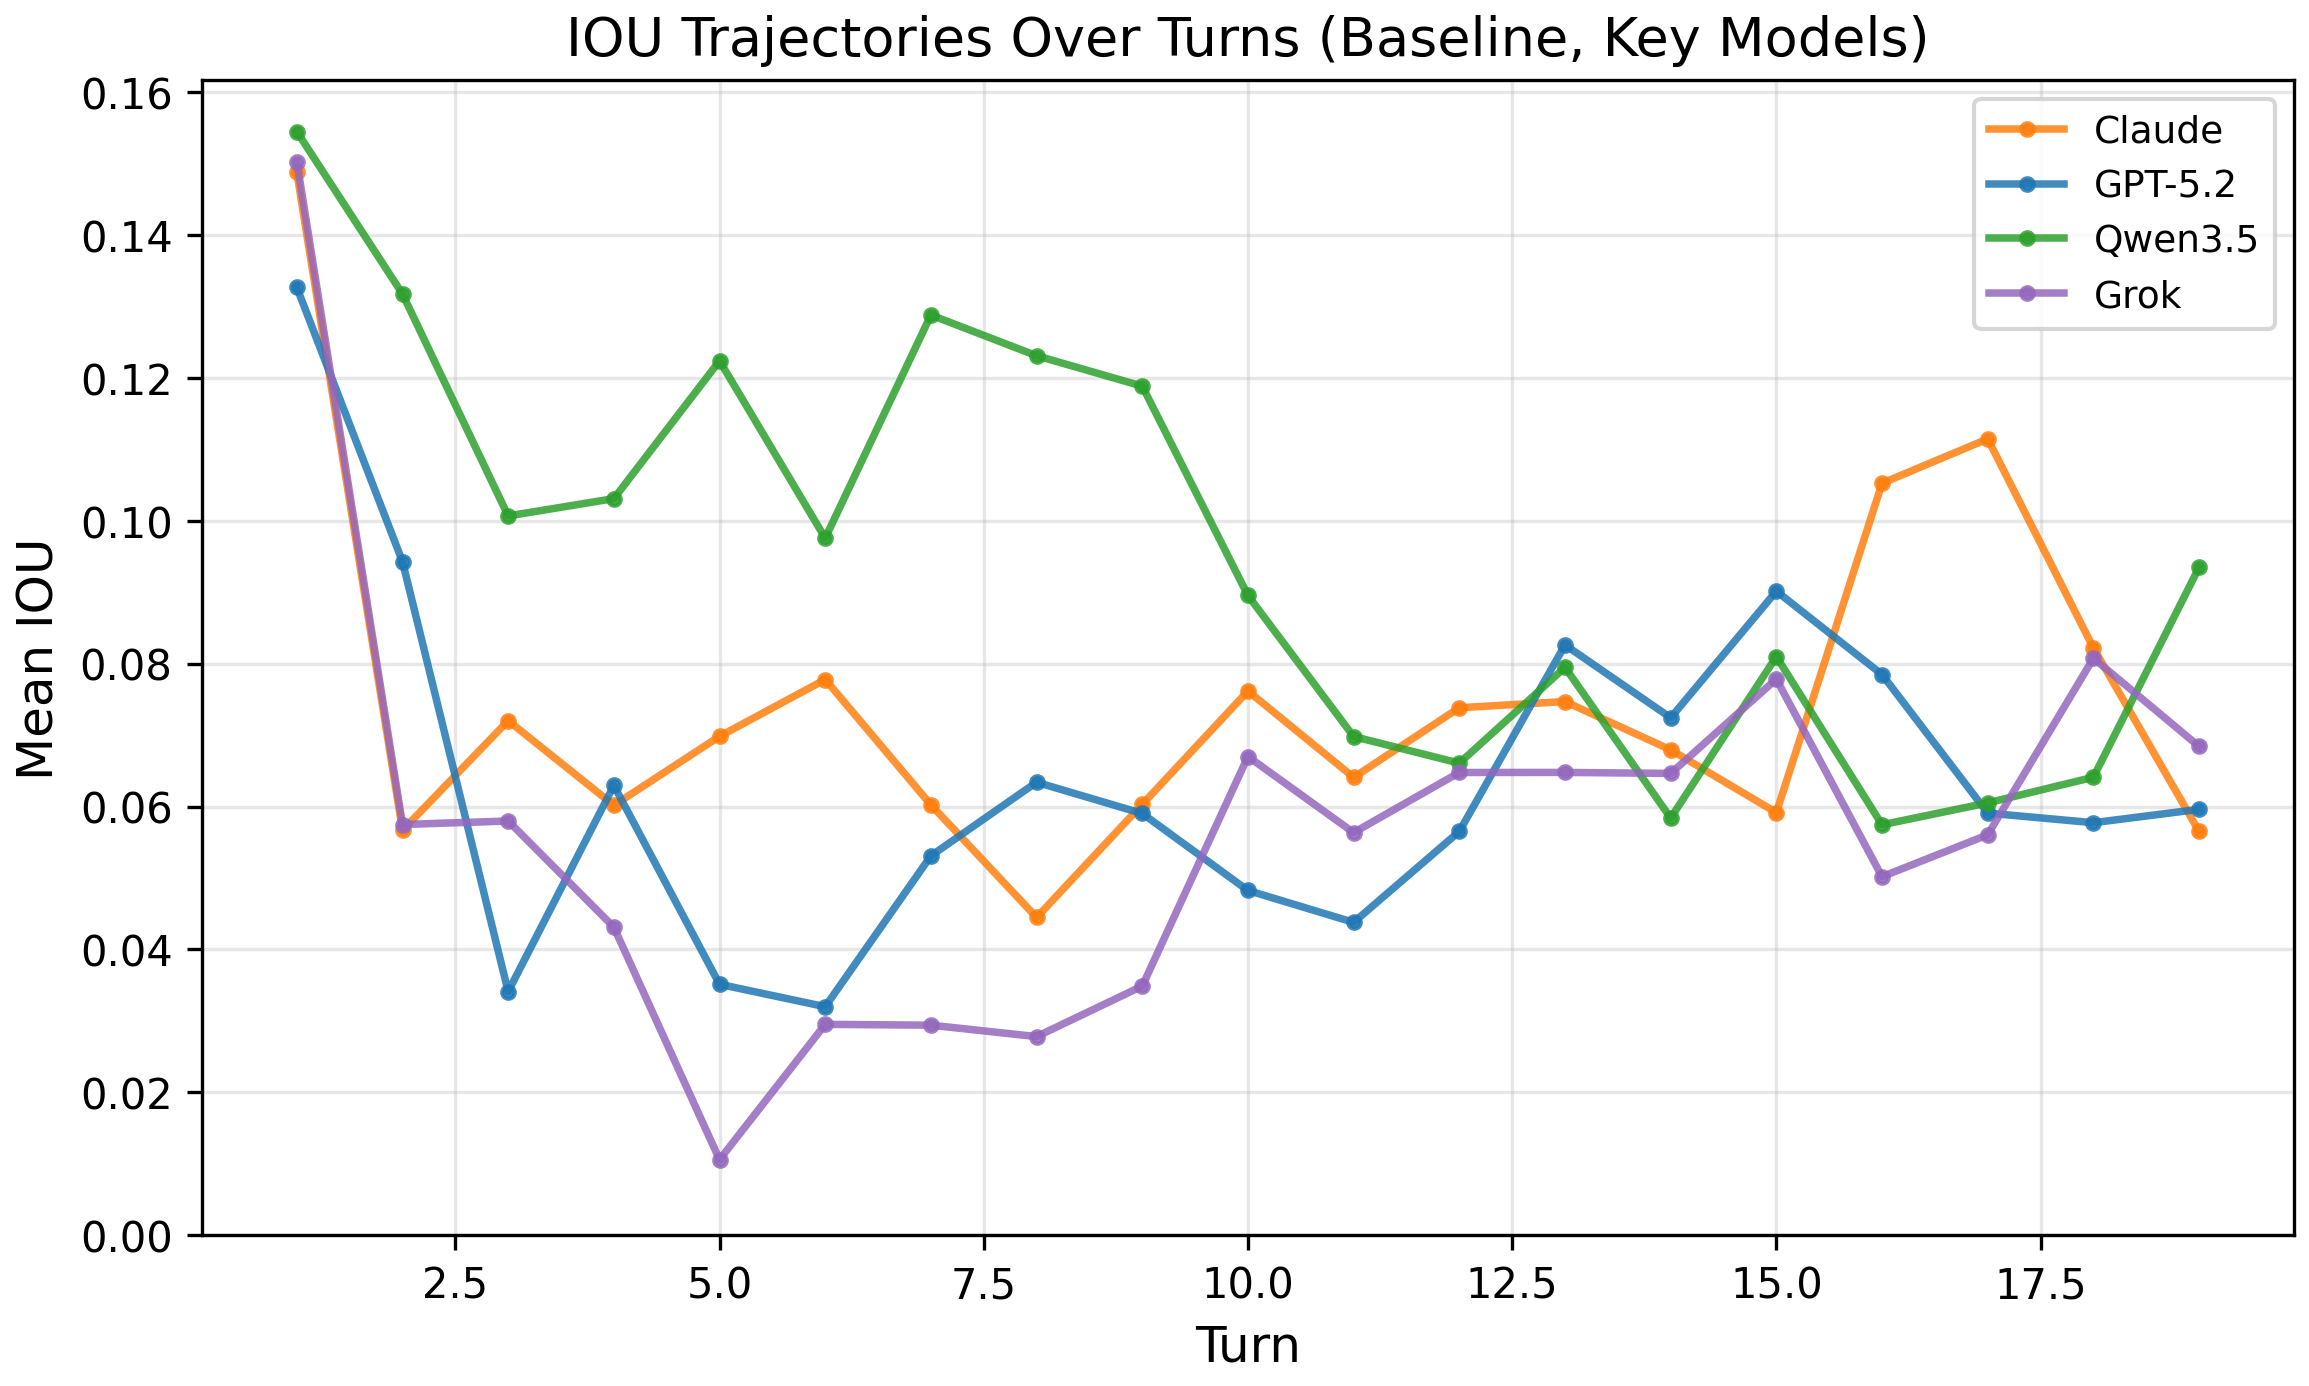
\includegraphics[width=0.8\textwidth]{../experiments_raw_results/wason-2-4-6/figures/wason246_iou_trajectories.png}
    \caption{Траектории среднего IOU по ходам диалога для четырёх ключевых стандартных моделей (baseline, без extended thinking). Все модели демонстрируют высокое начальное IOU с последующим постепенным снижением.}
    \label{fig:246_iou_trajectories}
\end{figure}

\begin{figure}[ht]
    \centering
    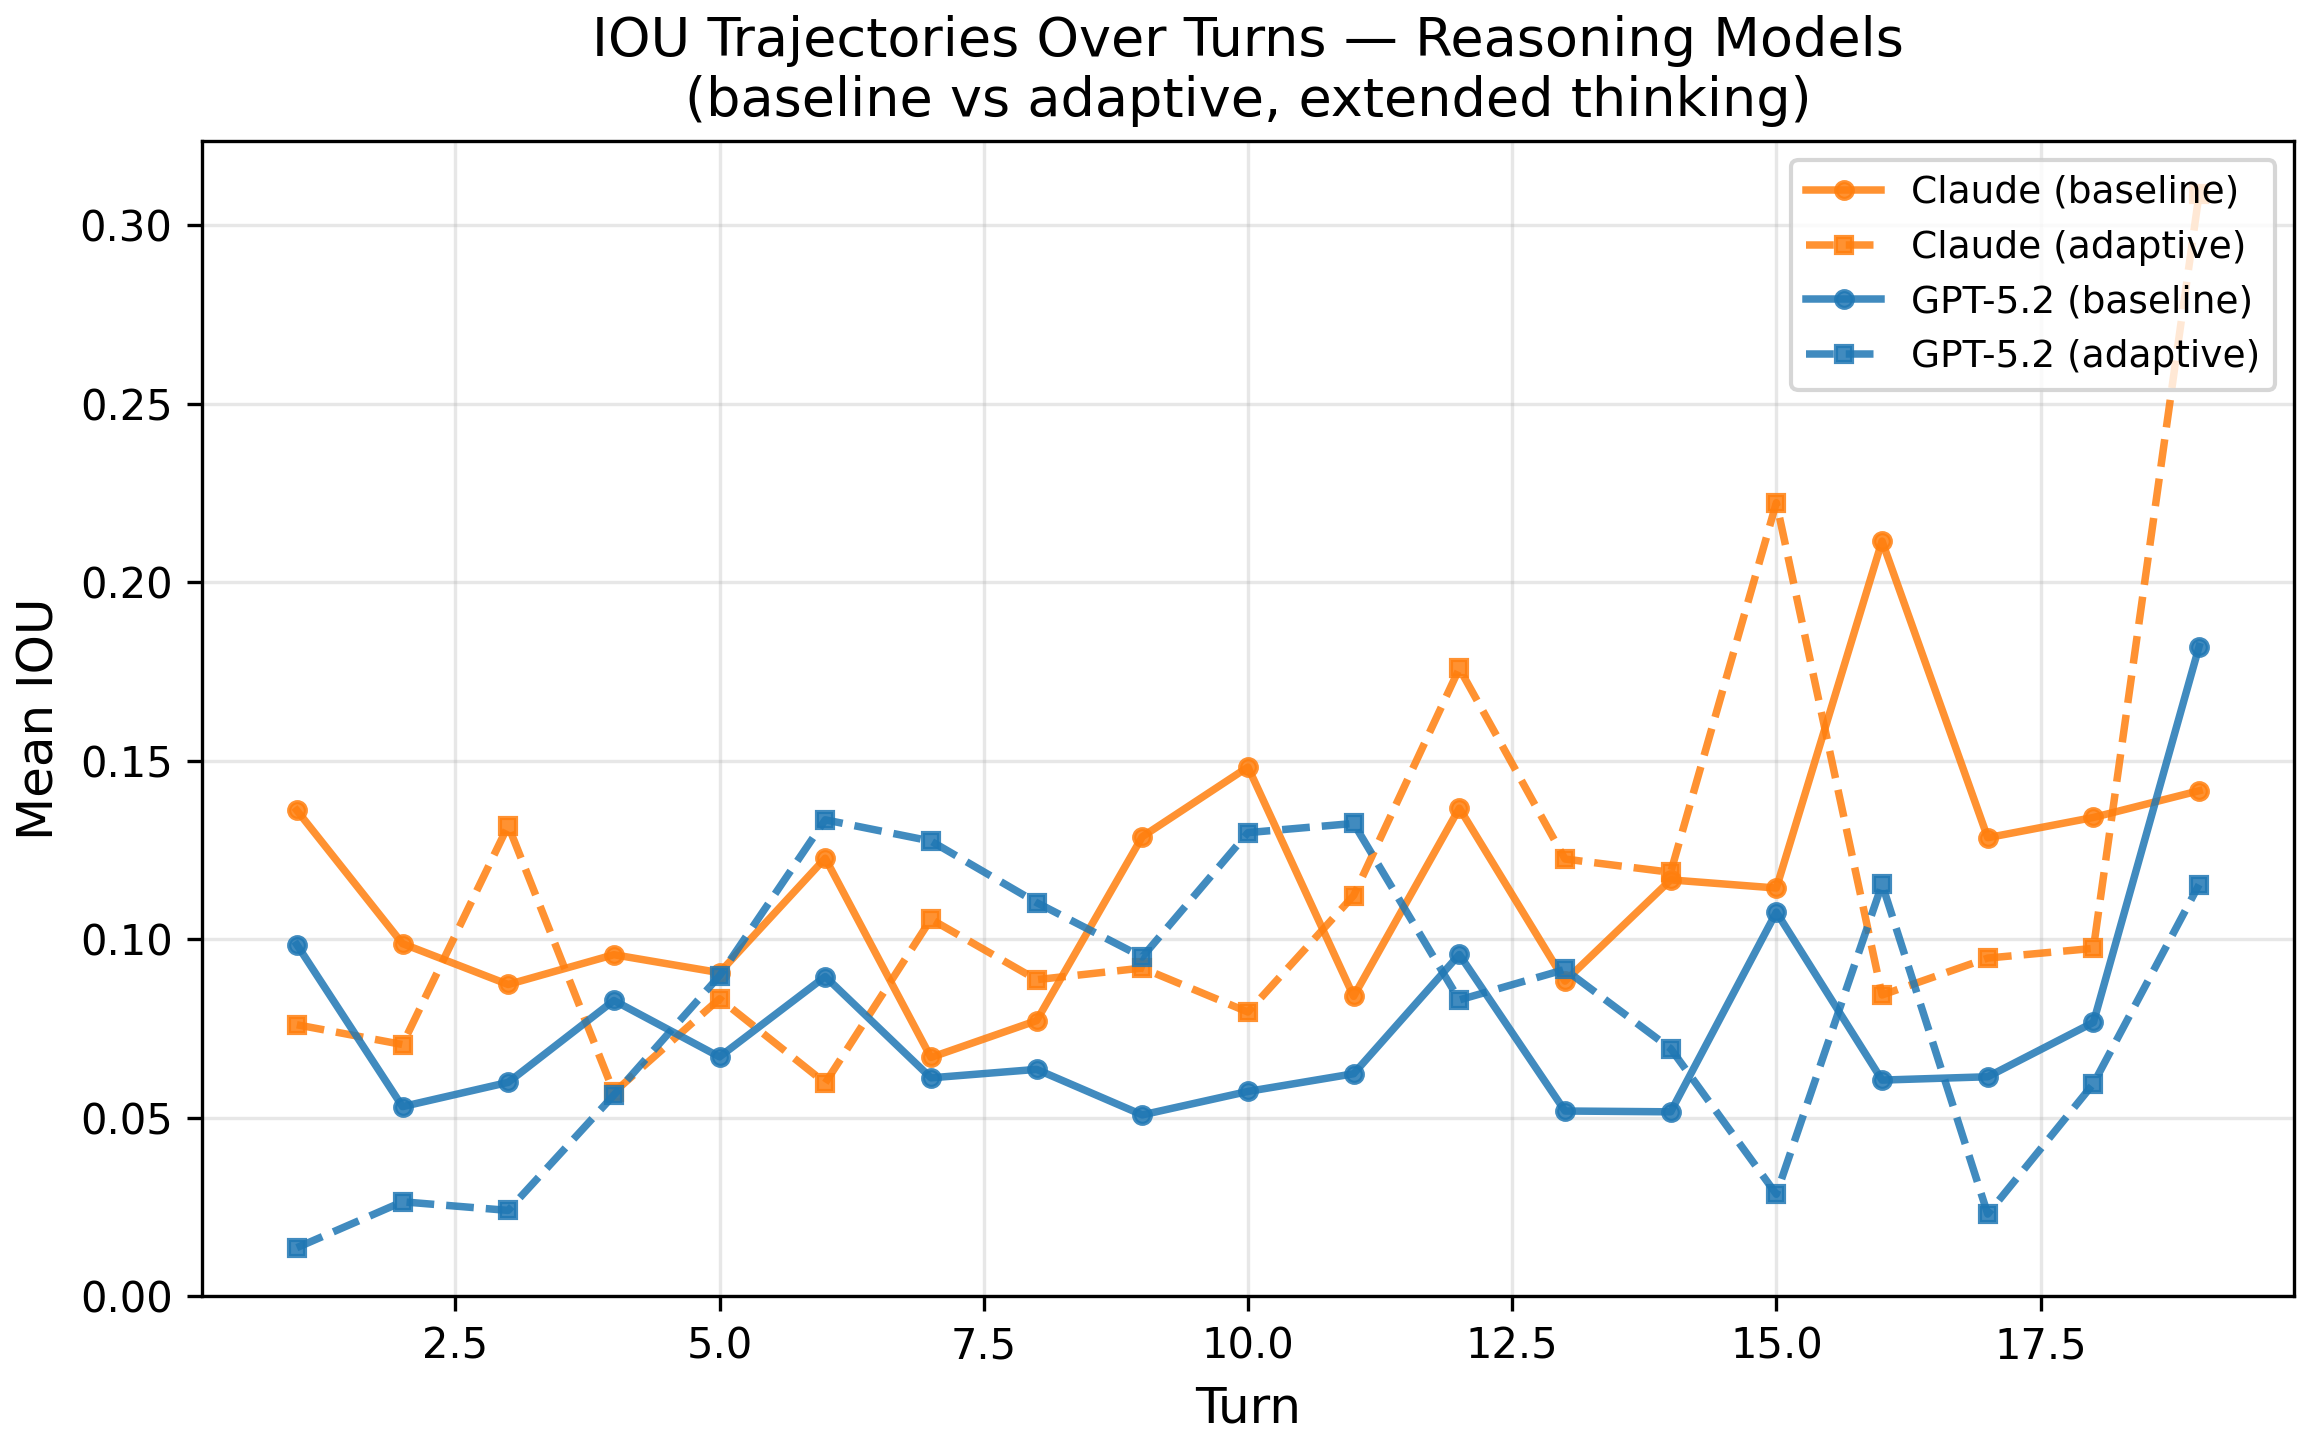
\includegraphics[width=0.8\textwidth]{../experiments_raw_results/wason-2-4-6/figures/wason246_reasoning_iou_trajectories.png}
    \caption{Траектории среднего IOU по ходам диалога для reasoning-моделей (extended thinking). Сплошные линии --- baseline-условие, пунктирные --- adaptive. В отличие от стандартных моделей, IOU у reasoning-моделей не монотонно снижается, а демонстрирует тенденцию к росту на поздних ходах, что свидетельствует о продолжении уточнения гипотезы.}
    \label{fig:246_iou_trajectories_reasoning}
\end{figure}

\textbf{Reasoning даёт качественный скачок.} Как видно на рис.~\ref{fig:246_iou_trajectories}, траектории Reasoning-моделей демонстрируют более быструю и устойчивую сходимость к истинному правилу. \texttt{gpt-5.2} в режиме reasoning (baseline) достигает SR $= 0{,}38$ --- на 10 процентных пунктов выше лучшей non-reasoning модели. В adaptive-условии SR вырастает до 0{,}48 и CTR снижается до 0{,}559, что является единственным случаем CTR ниже 0{,}60 во всём эксперименте. Примечательно, что \texttt{claude-sonnet-4.6 reasoning} также демонстрирует рост SR с 0,28 до 0,32 при адаптивном промпте. Таким образом, reasoning + adaptive --- единственная комбинация, приближающаяся к разумной фальсификационной стратегии, хотя и не достигающая нормативного стандарта.

\textbf{Adaptive-промпт нестабилен.} Из девяти non-reasoning моделей у четырёх SR не изменился или снизился (\texttt{gpt-5.2}: без изменений; \texttt{qwen3.5-397b-a17b}: $0{,}22 \to 0{,}18$; \texttt{grok-4.1-fast}: $0{,}14 \to 0{,}08$; \texttt{gemma-3-12b-it}: $0{,}06 \to 0{,}04$). Снижение CTR не гарантирует роста SR. На рис.~\ref{fig:246_scatter_sr_correlation} показана корреляция между стратегией тестирования (CTR) и итоговым успехом (SR) --- заметно, что снижение CTR помогает reasoning-моделям, но слабо влияет на эффективность большинства non-reasoning моделей.

\begin{figure}[ht]
    \centering
    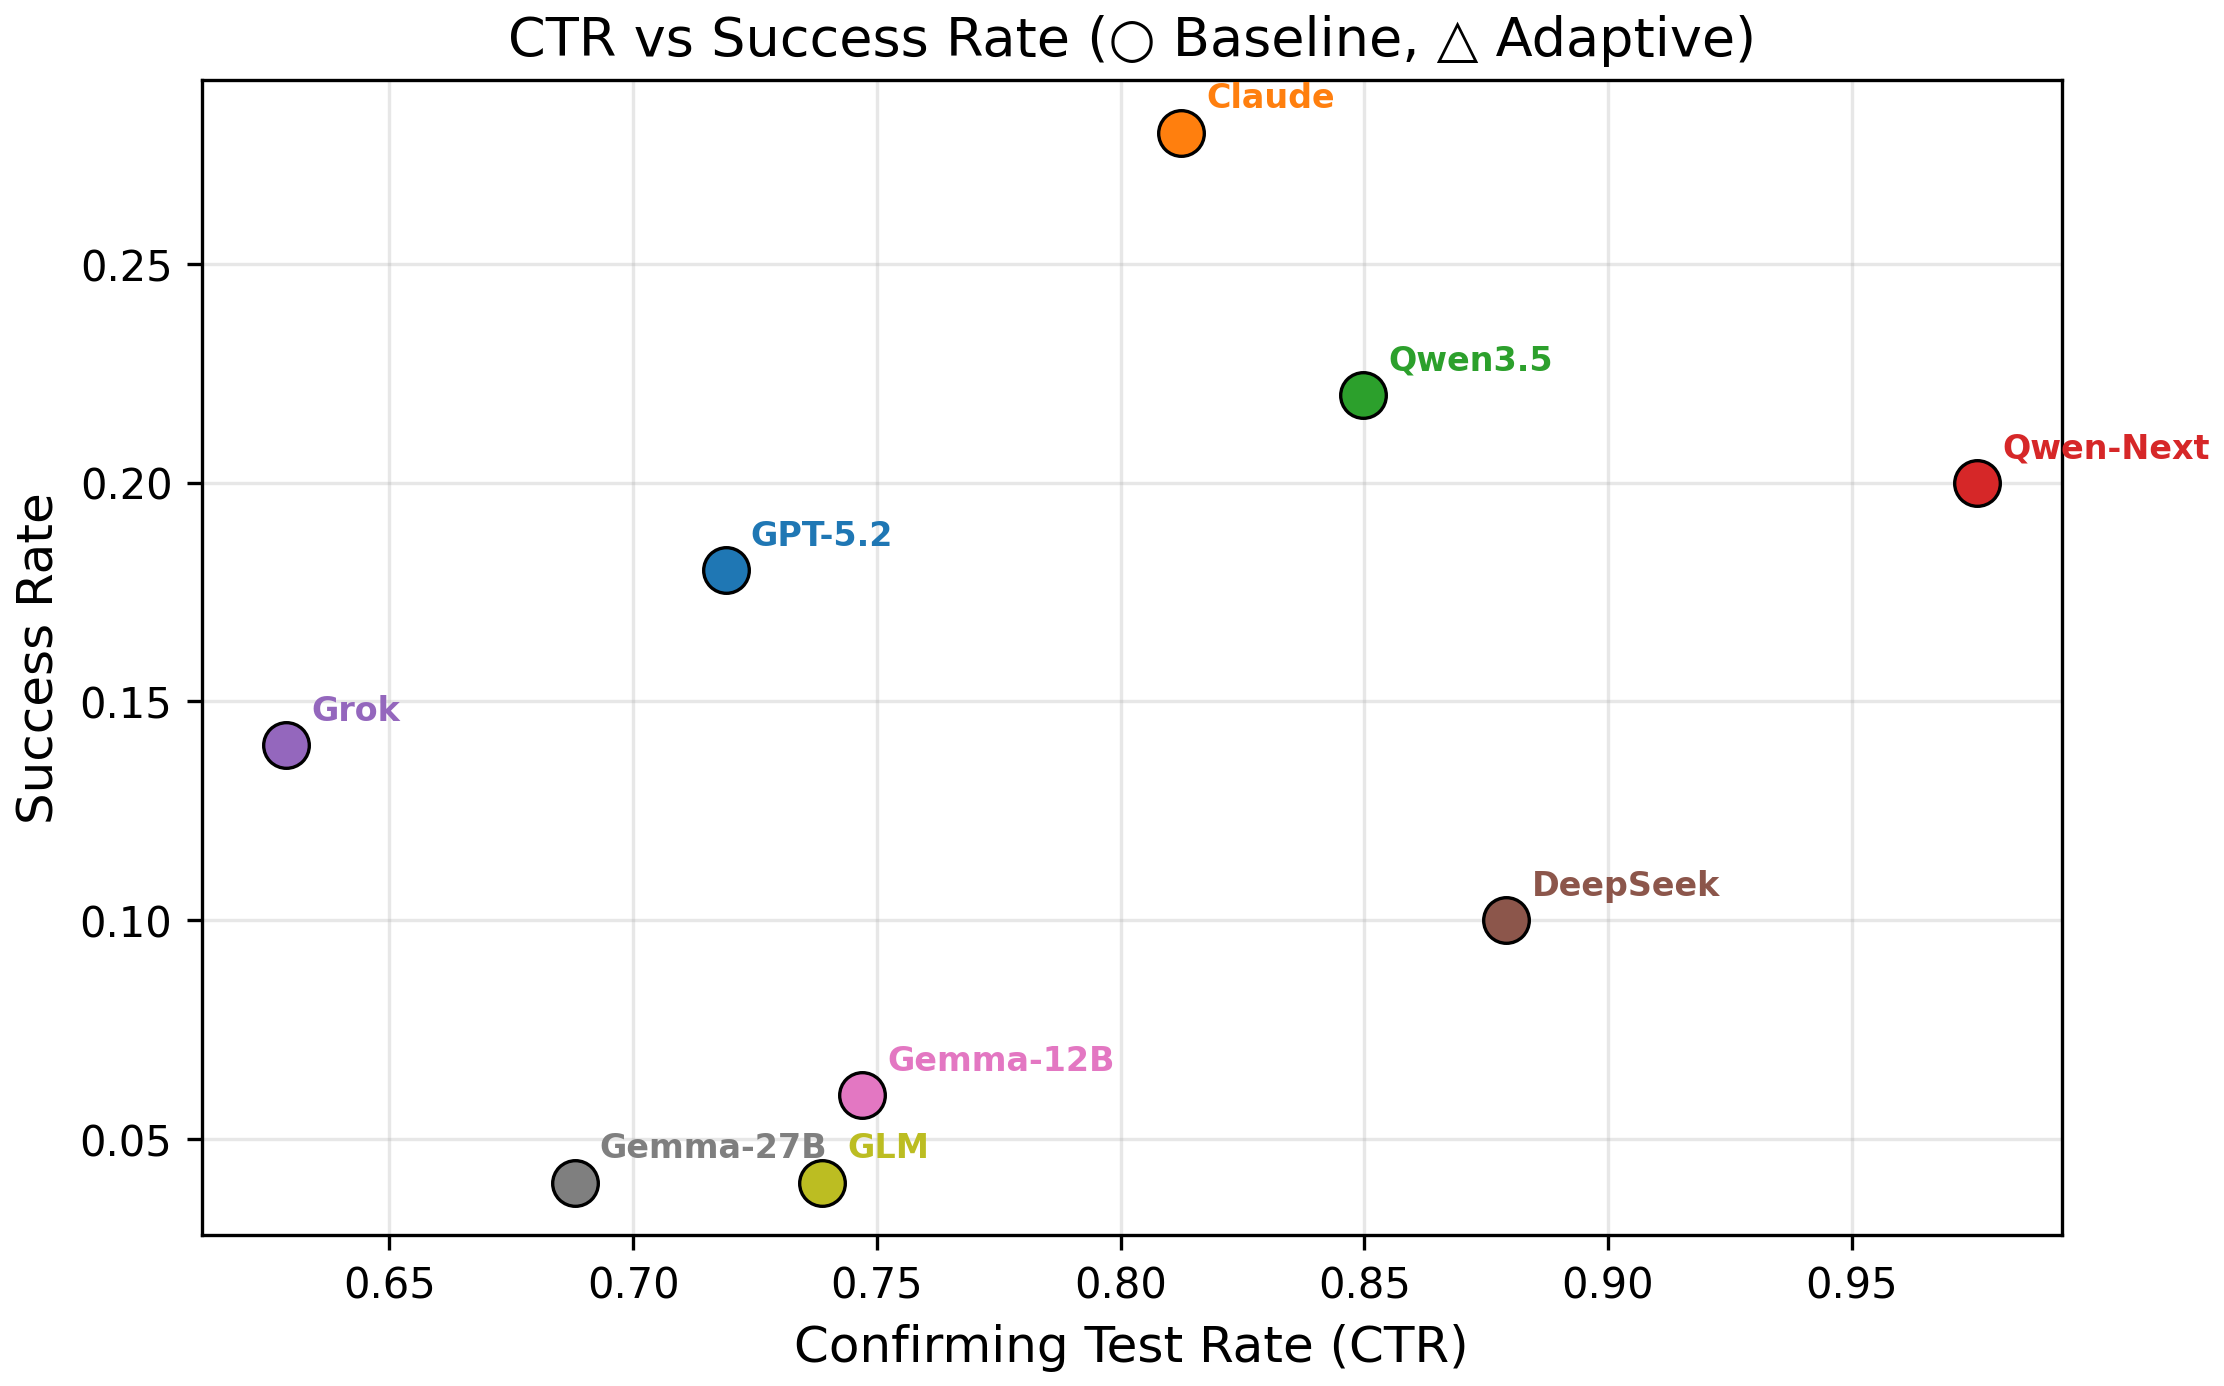
\includegraphics[width=0.8\textwidth]{../experiments_raw_results/wason-2-4-6/figures/wason246_scatter_sr_correlation.png}
    \caption{Корреляция между CTR и Success Rate. Пунктирная линия разделяет reasoning и non-reasoning модели.}
    \label{fig:246_scatter_sr_correlation}
\end{figure}

Наиболее интригующим является \textbf{парадокс \texttt{qwen3.5-397b-a17b}}: adaptive-промпт вызвал крупнейшее снижение CTR среди non-reasoning моделей ($0{,}850 \to 0{,}602$, то есть модель стала значительно активнее фальсифицировать), однако SR упал с 0{,}22 до 0{,}18. Модель начала тестировать опровергающие тройки, но не смогла конвертировать это в правильную гипотезу --- что указывает на разрыв между стратегией тестирования и качеством обновления гипотез.

\begin{figure}[ht]
    \centering
    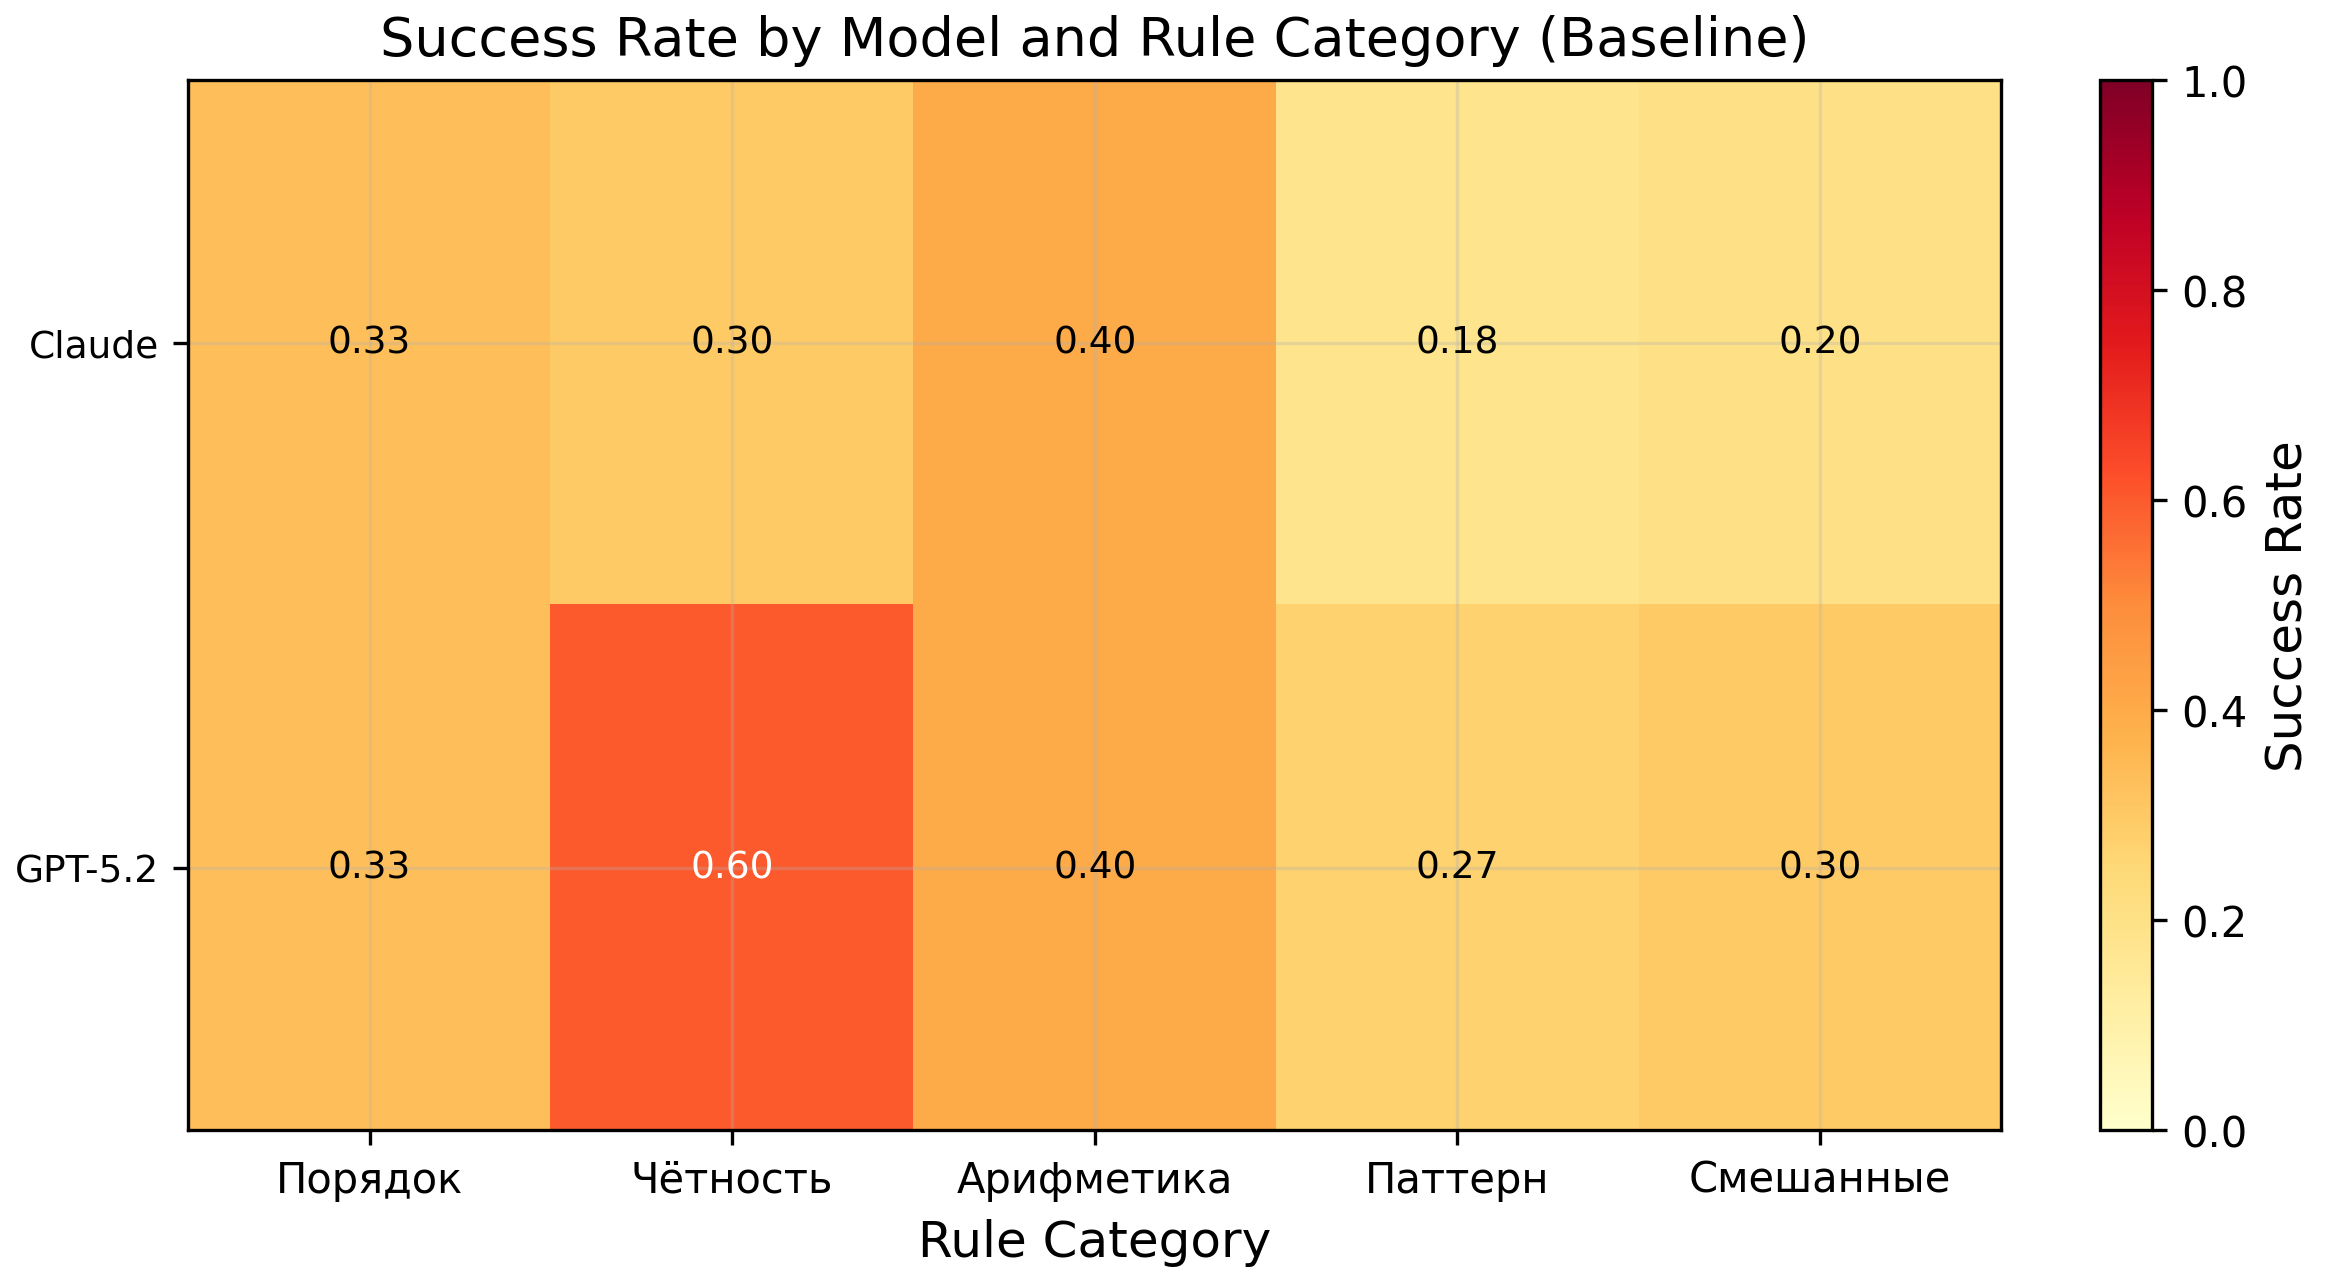
\includegraphics[width=0.9\textwidth]{../experiments_raw_results/wason-2-4-6/figures/wason246_category_heatmap.png}
    \caption{Тепловая карта Success Rate по категориям правил. Наибольшую сложность представляют структурные паттерны и смешанные правила.}
    \label{fig:246_category_heatmap}
\end{figure}

\textbf{Контринтуитивный эффект у \texttt{gemma-3-27b-it}:} adaptive-промпт, направленный на фальсификацию, \textit{увеличил} CTR ($0{,}688 \to 0{,}842$), однако SR при этом вырос с 0{,}04 до 0{,}10. Это указывает на то, что данная модель находит правильную гипотезу не через фальсифицирующую стратегию, а через какой-то иной механизм, нечувствительный к инструкциям по типу тестов. Анализ по категориям (рис.~\ref{fig:246_category_heatmap}) показывает, что категория «Структурные паттерны» (например, «ровно два уникальных значения») является наиболее труднодоступной для моделей, в то время как правила на порядок и сравнение («строго возрастающая последовательность») обнаруживаются значительно чаще.

\textbf{AUC-IOU} выявляет расхождение между качеством траектории и финальным результатом. У \texttt{gpt-5.2} reasoning при переходе baseline $\to$ adaptive: SR $+0{,}10$, но AUC-IOU $0{,}119 \to 0{,}082$ --- менее гладкая траектория сходимости при лучшем финальном результате. У \texttt{deepseek-v3.2} в baseline AUC-IOU ($0{,}052$) существенно ниже, чем у \texttt{claude-sonnet-4.6} ($0{,}127$), при схожем SR, что указывает на «спринт» к правильному ответу в последних ходах без устойчивого накопления качества гипотезы.

\begin{figure}[ht]
    \centering
    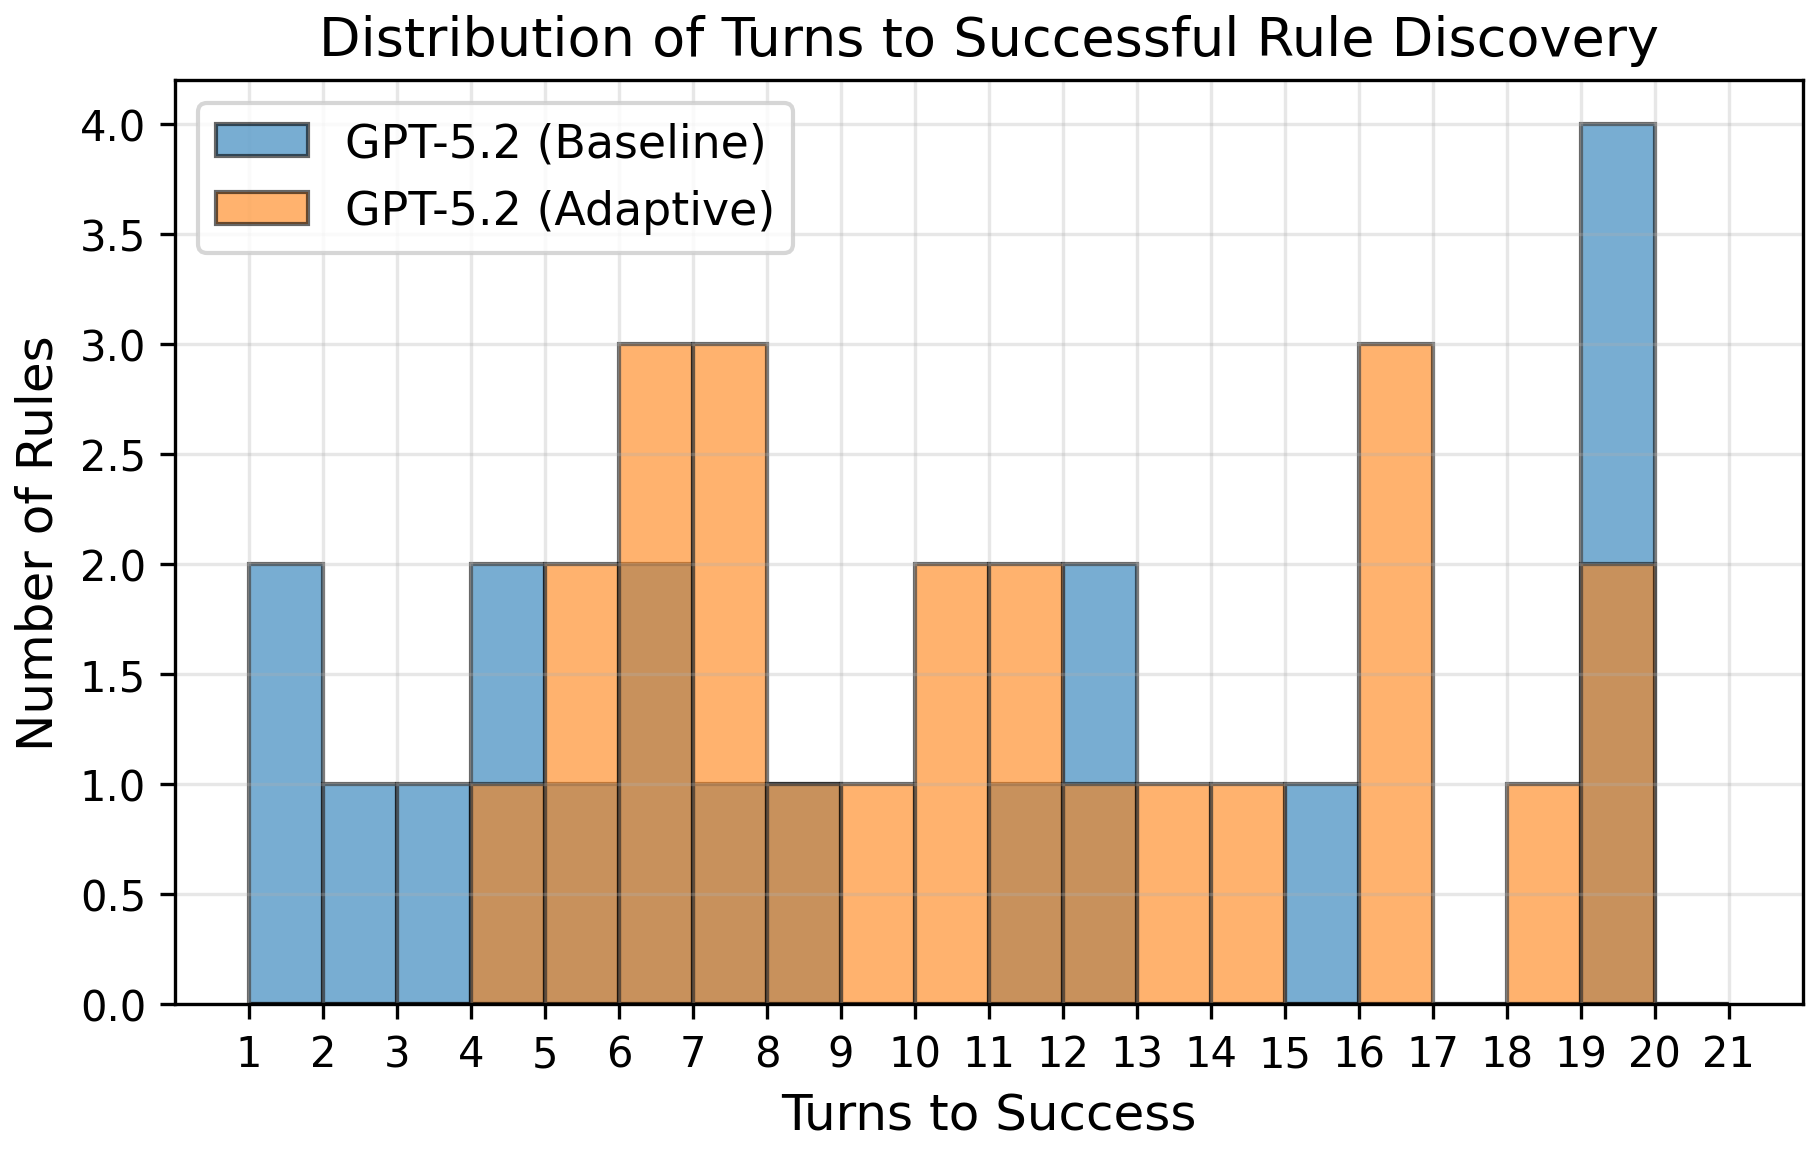
\includegraphics[width=0.7\textwidth]{../experiments_raw_results/wason-2-4-6/figures/wason246_turns_to_success.png}
    \caption{Среднее количество ходов до успешного обнаружения правила. Reasoning-модели приходят к решению существенно быстрее.}
    \label{fig:246_turns_to_success}
\end{figure}

\textbf{Hypothesis Change Rate (HCR)} в baseline варьируется от 0,622 у \texttt{gpt-5.2} до 0,940 у \texttt{gemma-3-27b-it}. Adaptive-промпт влияет на HCR неоднородно: у \texttt{deepseek-v3.2} HCR снижается с 0,833 до 0,595 (модель реже меняет гипотезу), у \texttt{gemma-3-27b-it} --- с 0,940 до 0,892, у \texttt{glm-4.7-flash} --- с 0,649 до 0,543. У ряда моделей (\texttt{qwen3.5-397b-a17b}: $0{,}654 \to 0{,}750$; \texttt{qwen3-next-80b}: $0{,}665 \to 0{,}732$) HCR при adaptive растёт --- модели активнее пересматривают гипотезы. Таким образом, adaptive-промпт влияет на поведение ревизии гипотез, однако это влияние не транслируется напрямую в рост SR. Как видно на рис.~\ref{fig:246_turns_to_success}, те модели, которые все же находят правило, в режиме Adaptive делают это за меньшее количество ходов.

\subsection{Выводы по эксперименту 3}

Эксперимент 3 установил: (1)~предубеждение подтверждения в индуктивном рассуждении универсально --- CTR $\geq 0{,}629$ у всех non-reasoning моделей в baseline; (2)~reasoning даёт качественный скачок, недостижимый через prompt engineering: SR \texttt{gpt-5.2} reasoning = 0{,}48 против максимума 0{,}28 у non-reasoning; (3)~adaptive-промпт нестабилен: снижение CTR не конвертируется в рост SR у половины моделей; (4)~парадокс \texttt{qwen3.5-397b-a17b} --- разрыв между стратегией тестирования и качеством обновления гипотез --- указывает на то, что предубеждение подтверждения имеет как минимум два независимых компонента: выбор тестируемых троек и ревизию гипотез.

% -------------------------------------------------------
\section{Сквозной анализ: три парадигмы, девять моделей}
% -------------------------------------------------------

\subsection{Сравнительная таблица результатов по всем экспериментам}

Таблица~\ref{tab:cross_experiment} представляет агрегированные результаты по всем трём экспериментам для каждой из девяти моделей.

\begin{table}[h!]
\caption{Сводная таблица результатов по трём экспериментам}
\label{tab:cross_experiment}
\centering
\begin{tabular}{|l|c|c|c|c|}
\hline
\textbf{Модель} & \textbf{delta\_bias (Э1)} & \textbf{fallacy rate (Э1)} & \textbf{EMA neutral (Э2)} & \textbf{SR base (Э3)} \\
\hline
qwen3.5-397b-a17b & $-0{,}005$ & $0{,}2\%$  & 0,764 & 0,22 \\
glm-4.7-flash     & $+0{,}028$ & $0{,}8\%$  & 0,332 & 0,04 \\
gemma-3-12b-it    & $+0{,}039$ & $2{,}9\%$  & 0,028 & 0,06 \\
claude-sonnet-4.6 & $+0{,}105$ & $0{,}2\%$  & 0,790 & 0,28 \\
deepseek-v3.2     & $+0{,}200$ & $18{,}7\%$ & 0,658 & 0,10 \\
grok-4.1-fast     & $+0{,}249$ & $22{,}9\%$ & 0,424 & 0,14 \\
gpt-5.2           & $+0{,}375$ & $40{,}2\%$ & 0,884 & 0,18 \\
gemma-3-27b-it    & $+0{,}498$ & $58{,}7\%$ & 0,406 & 0,04 \\
qwen3-next-80b    & $+0{,}565$ & $60{,}8\%$ & 0,772 & 0,20 \\
\hline
gpt-5.2 reasoning & ---        & ---        & ---   & 0,38 \\
\hline
\end{tabular}
\end{table}

\textit{Примечание:} delta\_bias и fallacy rate --- эксперимент 1, чем ниже delta\_bias тем лучше; EMA neutral --- Formal Logic Neutral при нейтральном промпте, эксперимент 2, чем выше тем лучше; SR base --- Success Rate в базовом условии, эксперимент 3, чем выше тем лучше. Таблица отсортирована по delta\_bias. \texttt{gpt-5.2} reasoning выделен отдельно как режим с принципиально иным типом вывода.

\subsection{Проверка гипотез о масштабировании и внутрисемейный парадокс}

Гипотеза H2 о снижении предубеждений с ростом модели получила частичное подтверждение. На уровне общей тенденции зависимость наблюдается: более мощные модели (\texttt{gpt-5.2}, \texttt{claude-sonnet-4.6}) систематически демонстрируют более низкий уровень предубеждений во всех трёх парадигмах. Однако внутри семейств картина неоднородна.

В семействе Gemma направление эффекта противоречит ожидаемому: \texttt{gemma-3-27b-it} демонстрирует несравнимо более высокий токен-bias (delta\_bias $= 0{,}498$, fallacy rate $58{,}7\%$), чем \texttt{gemma-3-12b-it} (delta\_bias $= 0{,}039$, fallacy rate $2{,}9\%$). Это является наиболее ярким проявлением внутрисемейного парадокса масштаба, зафиксированного в эксперименте 1. В семействе Qwen наблюдается противоположный паттерн: \texttt{qwen3-next-80b} при меньшем числе активных параметров демонстрирует существенно более высокий bias (delta\_bias $= 0{,}565$), чем \texttt{qwen3.5-397b-a17b} (delta\_bias $= -0{,}005$). Оба семейства указывают на то, что масштаб сам по себе не является надёжным предиктором устойчивости к когнитивным предубеждениям, и подчёркивают роль post-training alignment в формировании профиля предубеждений~\cite{batista2026rational}.

\textbf{Формальная проверка.} Для количественной оценки связи между масштабом и предубеждениями проведён ранговый корреляционный анализ Спирмена по шести открытым моделям с верифицируемым числом активных параметров: \texttt{gemma-3-12b-it} (12B), \texttt{qwen3.5-397b-a17b} (17B active), \texttt{gemma-3-27b-it} (27B), \texttt{glm-4.7-flash} (30B), \texttt{deepseek-v3.2} (37B active), \texttt{qwen3-next-80b} (80B). Проприетарные модели (\texttt{gpt-5.2}, \texttt{claude-sonnet-4.6}, \texttt{grok-4.1-fast}) исключены из анализа из-за отсутствия верифицируемых архитектурных данных; IKP-оценки~\cite{li2026ikp} дают лишь нижние границы с медианной погрешностью $1{,}59\times$, недостаточные для корреляционного анализа.

Результаты: $\rho_S$(active params, delta\_bias) $= 0{,}600$, $p = 0{,}208$; $\rho_S$(active params, EMA) $= 0{,}657$, $p = 0{,}156$; $\rho_S$(active params, SR) $= 0{,}116$, $p = 0{,}827$. Ни одна из корреляций не достигает значимости при $\alpha = 0{,}05$. Это формально подтверждает качественный вывод: при контроле по открытым моделям число активных параметров не является статистически значимым предиктором ни вероятностного предубеждения, ни дедуктивной компетентности, ни индуктивного успеха. Единственная умеренная положительная тенденция наблюдается для EMA ($\rho = 0{,}657$), однако она полностью обусловлена разницей между \texttt{gemma-3-12b-it} (EMA $= 0{,}106$) и остальными моделями и исчезает при исключении этой точки.

\subsection{Проверка гипотезы о спектральной природе предубеждений}

Гипотеза H3 подтверждена: уровень предубеждений систематически возрастает от эксперимента 1 к эксперименту 3. В задаче Линды в uncorrelated-условии ошибок нет ни у одной модели (все $n_{12} = 0$); в задаче Уэйсона EMA в нейтральном условии при нейтральном промпте не превышает 0,884 даже у лучшей модели, а у \texttt{gemma-3-12b-it} падает до 0,028; в задаче 2-4-6 CTR $> 0{,}60$ у всех моделей без исключения. Таким образом, индуктивное открытие правил остаётся наиболее уязвимой к предубеждению подтверждения областью для современных LLM, что согласуется с выводами Banatt и соавторов~\cite{banatt2024wilt} о тотальном доминировании стратегии позитивного тестирования, и с данными CogBench~\cite{coda2024cogbench} о систематическом разрыве между LLM и нормативными агентами именно в задачах фальсифицирующего поиска.

\subsection{Итоги: Proof-of-Concept фреймворка оценки когнитивных предубеждений}

Совокупность результатов трёх экспериментов позволяет сформулировать следующие итоговые положения.

Во-первых, когнитивные предубеждения в LLM являются устойчивым, воспроизводимым феноменом. Токен-bias зафиксирован у восьми из девяти моделей в эксперименте 1; предубеждение подтверждения в дедуктивном рассуждении --- у всех девяти в эксперименте 2; CTR $\geq 0{,}629$ у всех non-reasoning моделей в эксперименте 3. Гипотеза H1 подтверждена с оговоркой: \texttt{qwen3.5-397b-a17b} не проявляет значимого токен-bias в задаче Линды, однако демонстрирует выраженное предубеждение подтверждения в задачах Уэйсона и 2-4-6 (CTR $= 0{,}850$).

Во-вторых, профили предубеждений по экспериментам не коррелируют монотонно. Наглядный пример: \texttt{gpt-5.2} имеет высокий токен-bias в задаче Линды (fallacy rate $40{,}2\%$, delta\_bias $= 0{,}375$), но лучшую EMA в задаче Уэйсона ($0{,}884$) и наилучший SR в задаче 2-4-6 среди non-reasoning моделей ($0{,}18$, а в reasoning-режиме --- $0{,}38$). Это означает, что уязвимость к разным типам предубеждений не является единым латентным фактором, и ни одна агрегированная метрика не заменяет полного профиля.

В-третьих, масштаб модели не является надёжным предиктором устойчивости к предубеждениям, что согласуется с эффектами обратного масштабирования, описанными Dasgupta и соавторами~\cite{dasgupta2024language}. Внутрисемейный парадокс Gemma проявляется по-разному в разных экспериментах: в задаче Линды \texttt{gemma-3-27b-it} значительно хуже, чем \texttt{gemma-3-12b-it}; в задаче Уэйсона --- значительно лучше (EMA $0{,}578$ vs $0{,}106$); в задаче 2-4-6 обе модели слабы (SR $0{,}04$ и $0{,}06$). Это подчёркивает, что post-training alignment оказывает неоднородное воздействие на разные типы рассуждения~\cite{batista2026rational}.

В-четвёртых, reasoning является единственным вмешательством, дающим качественный скачок: SR \texttt{gpt-5.2} reasoning + adaptive ($0{,}48$) вдвое превышает лучший non-reasoning результат ($0{,}28$). Prompt engineering в форме CoT улучшает результаты только у моделей с достаточной базовой компетентностью и может давать обратный эффект у слабых моделей~\cite{kojima2022large}.



% ГЛАВА 3 - Практическая реализация
\chapter{ТЕХНИЧЕСКАЯ РЕАЛИЗАЦИЯ ЭКСПЕРИМЕНТАЛЬНОГО ФРЕЙМВОРКА}

% -------------------------------------------------------
\section{Архитектура воспроизводимого экспериментального фреймворка}
% -------------------------------------------------------

\subsection{Общая структура кодовой базы}

Экспериментальный фреймворк реализован в виде единого Python-проекта с общей инфраструктурой и тремя независимыми экспериментальными модулями. Управление зависимостями осуществляется через менеджер пакетов \texttt{uv} с фиксированным lockfile, что обеспечивает побайтовую воспроизводимость окружения. Минимальная требуемая версия интерпретатора~--- Python~3.12.

Структура проекта:
\begin{itemize}
  \item \texttt{src/common/} --- общая инфраструктура: асинхронный клиент OpenRouter (\texttt{openrouter.py}), утилита загрузки данных из Google Sheets (\texttt{google\_sheets.py}), учёт потреблённых токенов;
  \item \texttt{common\_config.py} --- централизованная конфигурация: базовый URL API, список тестируемых моделей, загрузка ключа из переменной окружения \texttt{OPENROUTER\_API\_KEY};
  \item \texttt{linda-problem/} --- эксперимент 1: \texttt{run\_experiments.py}, \texttt{compute\_metrics.py}, \texttt{generate\_dataset.py}, \texttt{config.py};
  \item \texttt{wason-selection/} --- эксперимент 2: \texttt{run\_experiments.py}, \texttt{compute\_metrics.py}, \texttt{download\_inputs.py}, \texttt{build\_graphs.py}, \texttt{upload\_results.py};
  \item \texttt{wason-2-4-6/} --- эксперимент 3: \texttt{run\_experiments.py}, \texttt{metrics.py}, \texttt{compute\_metrics.py}, \texttt{build\_graphs.py};
  \item \texttt{tests/} --- unit-тесты для всех трёх экспериментальных модулей.
\end{itemize}

Основные зависимости: \texttt{openai} (клиент OpenRouter), \texttt{pandas}, \texttt{numpy}, \texttt{scipy}, \texttt{scikit-learn} (статистический анализ), \texttt{matplotlib}, \texttt{seaborn} (визуализация), \texttt{pydantic} (валидация конфигураций), \texttt{google-auth}, \texttt{gspread} (интеграция с Google Sheets).

Все три эксперимента запускаются через единый интерфейс командной строки:
\begin{itemize}
  \item эксперимент 1: \texttt{uv run python linda-problem/run\_experiments.py {-}{-}api-key \$OPENROUTER\_API\_KEY}
  \item эксперимент 2: \texttt{uv run python wason-selection/run\_experiments.py {-}{-}models <model\_id> {-}{-}api-key \$OPENROUTER\_API\_KEY}
  \item эксперимент 3: \texttt{uv run python wason-2-4-6/run\_experiments.py {-}{-}models <model\_id> {-}{-}prompt-style adaptive {-}{-}reasoning-effort none {-}{-}api-key \$OPENROUTER\_API\_KEY}
\end{itemize}

\subsection{Унифицированный API-интерфейс и маршрутизация моделей}

Ключевым архитектурным решением является использование единого прокси-маршрутизатора OpenRouter (\texttt{https://openrouter.ai/api/v1}) для запросов ко всем моделям. Это устраняет артефакты, связанные с различиями в препроцессинге промптов, системных сообщениях и токенизации у разных провайдеров. Все модели запрашиваются через идентичный клиент на базе библиотеки \texttt{openai} с базовым URL OpenRouter.

Модели конфигурируются централизованно в \texttt{common\_config.py}. Список тестируемых моделей включает девять систем:
\begin{itemize}
  \item \textbf{Проприетарные:} \texttt{gpt-5.2} (OpenAI), \texttt{claude-sonnet-4.6} (Anthropic), \texttt{grok-4.1-fast} (xAI);
  \item \textbf{Открытые:} \texttt{qwen3-next-80b}, \texttt{qwen3.5-397b-a17b} (Alibaba), \texttt{deepseek-v3.2} (DeepSeek), \texttt{gemma-3-27b-it}, \texttt{gemma-3-12b-it} (Google), \texttt{glm-4.7-flash} (Zhipu AI).
\end{itemize}

Выбор моделей обеспечивает: (1) различных провайдеров, (2) различные парадигмы доступа (закрытые API и open-weight модели), (3) широкий спектр параметров (от компактных моделей 12B до масштабных систем 397B). Использование единого прокси гарантирует идентичность конфигурации запросов: формат системного сообщения, роль user/assistant и параметры токенизации остаются неизменными при переключении между моделями.

% -------------------------------------------------------
\section{Параметры запросов и механизм отказоустойчивости}
% -------------------------------------------------------

\subsection{Конфигурация параметров по экспериментам}

Параметры запросов к API дифференцируются в зависимости от методологических требований каждого эксперимента.

\textbf{Эксперимент 1 (задача Линды).} Использовались \texttt{temperature=0.0} для обеспечения максимальной детерминированности бинарного выбора, \texttt{max\_completion\_tokens=160} (достаточно для выбора опции и указания уверенности), \texttt{seed=42}. Конкурентность~--- 20 одновременных запросов, 4 попытки при ошибках, таймаут 60 секунд. Нулевая температура обусловлена требованием воспроизводимости: при повторном запросе той же виньетки модель должна вернуть идентичный ответ.

\textbf{Эксперимент 2 (задача Уэйсона).} Использовалась \texttt{temperature=1.0}, \texttt{max\_completion\_tokens=1000}, \texttt{random\_seed=42}. Единица температуры выбрана намеренно: систематические перестановки карточек (5 перестановок на правило) требуют естественной вариабельности ответов для оценки стабильности. При \texttt{temperature=0} модель могла бы выдавать идентичный ответ на все перестановки, что сделало бы невозможной оценку Consistency Rate как самостоятельной метрики. Конкурентность~--- до 60 одновременных запросов.

\textbf{Эксперимент 3 (задача 2-4-6).} Использовались \texttt{temperature=0}, \texttt{max\_turns=19}, таймаут 120 секунд на каждый многоходовой диалог, до 50 одновременных запросов. Нулевая температура обеспечивает стабильность генерации гипотез в рамках одного испытания. Максимальное число ходов (19) выбрано эмпирически: это обеспечивает достаточный горизонт для обнаружения правила, не приводя к избыточным затратам API.

\subsection{Механизм повторных попыток и repair-протокол}

Механизм повторных попыток при ошибках реализован через экспоненциальный backoff по формуле:
\begin{equation}
  \text{delay} = \min(2^{(\text{attempt}-1)}, 8) + U(0; 0{,}25) \text{ сек},
  \label{eq:backoff}
\end{equation}
где \texttt{attempt} --- номер текущей попытки (начиная с 1), а $U(0; 0{,}25)$~--- случайная добавка для предотвращения синхронизации запросов. Максимальная задержка ограничена 8 секундами.

В эксперименте 3, где требуется строго форматированный ответ (блок \texttt{```python```} с двумя строками: гипотеза и тройка), реализован дополнительный \textit{repair-протокол}. После каждого невалидного ответа формируется repair-prompt с явным указанием нарушенного требования формата:
\begin{quote}
\textit{Your previous response was invalid because: [reason]. Please respond again with EXACTLY this format: \texttt{```python H: lambda x, y, z: <hypothesis> T: [x, y, z] ```}}
\end{quote}

Выполняется до 2 дополнительных попыток ремонта. Типичные причины невалидности: выход значений за диапазон $[1, 1000]$, неполный блок (отсутствие гипотезы или тройки), использование граничных значений 0 или 1001. Все случаи нарушения формата записываются в \texttt{format\_errors.jsonl} для последующего аудита.

Наибольшее число ошибок формата зафиксировано у \texttt{grok-4.1-fast} (23 ошибки), \texttt{deepseek-v3.2} (14), \texttt{gemma-3-27b-it} (9) и \texttt{qwen3-next-80b} (7). У трёх моделей зафиксированы невалидные правила в финальном прогоне (\texttt{gemma-3-27b-it}: 2, \texttt{deepseek-v3.2}: 1, \texttt{qwen3-next-80b}: 1), исключённые из подсчёта Success Rate.

% -------------------------------------------------------
\section{Структура и генерация датасетов}
% -------------------------------------------------------

\subsection{Эксперимент 1: биографические виньетки с факториальными подстановками}

Основной датасет \texttt{linda-problem/data/conjunction\_dataset\_all.csv} содержит 130 оригинальных биографических виньеток, составленных вручную. Каждая виньетка описывает персонажа с выраженными личностными характеристиками и содержит плейсхолдеры \texttt{\{NAME\}}, \texttt{\{RACE\}} и \texttt{\{AGE\}}, заменяемые в ходе подстановки.

К каждой виньетке прилагаются пять элементов: простая опция T (профессия), коррелированное хобби F, некоррелированное хобби F\_uncorrelated и две конъюнктивные опции T\_and\_F1 и T\_and\_F2. Профессии сэмплировались из базы статистики занятости USDL/OEWS~\cite{usdl2024oews}, насчитывающей около 830 профессиональных категорий, что обеспечивает разнообразие и репрезентативность стимульного материала.

\textbf{Механизм подстановки.} Операция строковой замены (string replacement) применяется к плейсхолдерам каждой виньетки. Имена подбирались так, чтобы однозначно ассоциироваться с расовой группой согласно данным о частотности имён в США: White (Emma, James), Black (Jamal, Aisha), Hispanic (Carlos, Maria), Asian (Wei, Priya). Возрасты: 24, 38, 55 лет.

Первоначально эксперимент проводился на полной факториальной сетке: 8 имён $\times$ 3 возраста = 24 варианта подстановки на виньетку, что давало 3120 пар испытаний. После анализа результатов первых двух моделей (\texttt{glm-4.7-flash} и \texttt{qwen3.5-397b-a17b}), показавшего незначимость возрастного и proxy-gender эффектов (delta\_bias по возрастным группам в диапазоне $-0{,}005 \div +0{,}003$), сетка была сокращена до расово-значимых подстановок: 4 расовые группы $\times$ 1 имя $\times$ 1 возраст = 520 пар испытаний на модель. Данное решение, хотя и обоснованное промежуточными результатами, ограничивает возможность сравнительного анализа расового эффекта по всем девяти моделям.

\subsection{Эксперимент 2: пять контентных условий}

Пять датасетов хранятся в директории \texttt{wason-selection/input/}, каждый по 100--101 записи в формате CSV со столбцами \texttt{Rule Text} (текстовая формулировка правила) и \texttt{JSON Mapping} (отображение поверхностных значений на логические роли P, $\lnot$P, Q, $\lnot$Q).

\textbf{Протокол перестановок.} Ключевым методологическим элементом является систематическая манипуляция порядком предъявления карточек. Каждый стимул предъявлялся каждой модели в \textbf{пяти различных перестановках} четырёх позиций карточек. Дизайн следует из наблюдения Binz и Schulz~\cite{binz2023using} о том, что единственное изменение перестановки способно обратить ответ GPT-3 на каноническую задачу. Данный подход даёт \textbf{500 испытаний на модель на условие} (100 правил $\times$ 5 перестановок), позволяя оценивать распределения ответов, а не точечные оценки.

\subsection{Эксперимент 3: пятьдесят верифицированных правил}

Набор из 50 правил хранится в Google Sheets и загружается при запуске через \texttt{google\_sheets.py}. Локально сохранён манифест \texttt{wason-2-4-6/output/adaptive/none/rules\_manifest.csv} (50 строк, столбцы \texttt{code} и \texttt{category}), где \texttt{code}~--- исполняемое Python lambda-выражение вида \texttt{lambda x, y, z: x < y < z}.

Правила организованы в пять таксономических категорий: порядок и сравнение (9 правил), чётность и делимость (10), арифметические отношения (10), структурные паттерны (11), смешанные/составные (10). Все правила верифицированы на: (1) исполнимость в диапазоне $[1, 99]^3$, (2) отсутствие функциональных дубликатов (через экстенсиональную эквивалентность), (3) отсутствие тавтологий. Из 50 правил 26 удовлетворяются тройкой $(2, 4, 6)$ и 24 не удовлетворяются, что обеспечивает сбалансированную выборку для тестирования.

% -------------------------------------------------------
\section{Реализация метрик и статистического протокола}
% -------------------------------------------------------

\subsection{Метрика экстенсиональной эквивалентности (IOU)}

Ключевой методологической особенностью эксперимента 3 является оценка гипотез через экстенсиональную эквивалентность вместо текстового сравнения строк. Функция \texttt{compare\_sets(R, H, n=200000)} реализует следующий алгоритм: правило $R$ и гипотеза $H$ компилируются в Python lambda через \texttt{eval}; затем генерируется Монте-Карло-выборка из 200\,000 случайных троек $(x, y, z) \in [1, 1000]^3$ через \texttt{numpy.random.randint}; для каждой тройки вычисляются булевы векторы принадлежности, по которым считаются $|\mathbf{h}_t \cap \mathbf{r}|$, $|\mathbf{h}_t \cup \mathbf{r}|$ и итоговый IOU по формуле~\eqref{eq:iou}.

Для метрики изменения гипотез (HCR) используется отдельно кэшированная выборка из 50\,000 троек (\texttt{HYPOTHESIS\_CHANGE\_SAMPLES}), что снижает вычислительную нагрузку при сравнении пар последовательных гипотез. Использование \texttt{eval} для компиляции lambda-выражений оправдано тем, что все правила верифицированы и имеют фиксированный формат \texttt{lambda x, y, z: <expression>}, не допускающий произвольного выполнения кода.

\subsection{Метрика Severity of Bias и протокол уверенности}

В эксперименте 1 реализована непрерывная метрика силы предубеждения, основанная на самооценке уверенности модели. Функция \texttt{compute\_bias\_score(choice, confidence)} реализует следующую логику: при выборе конъюнкции (b) $\text{bias\_score} = \text{confidence} / 100$; при выборе T (a) $\text{bias\_score} = (100 - \text{confidence}) / 100$. Шкала от 0 (минимальное предубеждение) до 1 (максимальное предубеждение).

Агрегированная метрика delta\_bias вычисляется как разность средних bias\_score между correlated- и uncorrelated-условиями по формуле~\eqref{eq:delta_bias}. Эта величина отражает чистый эффект нарративной связности, очищенный от фонового уровня неуверенности модели. Парсинг уверенности реализован через regex-паттерн, извлекающий числовое значение из второй строки ответа модели.

\subsection{Статистический протокол: McNemar, Cohen's \textit{d}, FDR-коррекция}

Статистический вывод в эксперименте 1 основан на точном тесте МакНемара для согласованных пар бинарных наблюдений~\cite{mcnemar1947note}. Для каждой пары испытаний (correlated, uncorrelated) одной подставленной виньетки строилась таблица сопряжённости 2$\times$2. При $n^* = n_{12} + n_{21} > 10$ использовалась нормальная аппроксимация со статистикой $z_0 = (n_{21} - n_{12}) / \sqrt{n_{21} + n_{12}}$.

Размер эффекта оценивается через Cohen's $d = t / \sqrt{n}$, где $t$~--- значение парной t-статистики, $n$~--- число пар наблюдений. Пороги интерпретации: $0{,}2$~--- малый эффект, $0{,}5$~--- умеренный, $0{,}8$~--- большой, $>1{,}0$~--- очень большой.

При множественных сравнениях (например, между демографическими группами) применяется процедура коррекции $p$-значений Бенджамини-Хохберга (BH-FDR)~\cite{benjamini1995controlling} для контроля частоты ложных открытий на уровне $\alpha = 0{,}05$.

\subsection{Метрики дедуктивного рассуждения: EMA, MBI, CBR, Consistency Rate}

В эксперименте 2 реализованы четыре метрики. \textbf{Expected Metric Accuracy (EMA)}~--- доля испытаний с нормативно правильным набором $\{$P, $\lnot$Q$\}$. \textbf{Matching Bias Index (MBI)}~--- доля испытаний с выбором $\{$P, Q$\}$. \textbf{Confirmation Bias Rate (CBR)}~--- доля испытаний с выбором только $\{$P$\}$. \textbf{Consistency Rate}~--- доля правил, для которых модель даёт идентичный выбор карточек во всех пяти перестановках.

Все метрики вычисляются функцией \texttt{compute\_metrics.py}, которая принимает JSON-лог сырых ответов модели и отображение логических ролей карточек, возвращает агрегированные значения по каждому контентному условию и промпт-условию.

% -------------------------------------------------------
\section{Технические проблемы и их решения}
% -------------------------------------------------------

\subsection{Нарушения формата ответа в многоходовом диалоге}

Наиболее значимой технической проблемой стали систематические нарушения формата ответа в эксперименте 3. Модели должны были отвечать строго в блоке \texttt{```python```} с двумя строками: гипотеза (\texttt{H: lambda x, y, z: ...}) и тестируемая тройка (\texttt{T: [x, y, z]}). На практике модели генерировали: пояснительный текст за пределами блока, тройки с отрицательными или нулевыми значениями, тройки с числами свыше 1000, неполные блоки без гипотезы или без тройки.

Решение: двухуровневый механизм валидации. На первом уровне regex-парсер извлекает блок \texttt{```python```} и проверяет наличие обоих обязательных элементов. На втором уровне выполняется семантическая валидация: все числа тройки проверяются на принадлежность диапазону $[1, 1000]$, а гипотеза~--- на синтаксическую корректность через \texttt{compile()}. При невалидности срабатывает repair-протокол (см.~раздел~3.2.2) с указанием конкретной причины ошибки.

\subsection{Ограничение конкурентности и квоты API}

При массовом запуске эксперимента 2 (9 моделей $\times$ 5 условий $\times$ 5 перестановок $\times$ 100 правил = 22\,500 запросов) и эксперимента 3 (9 моделей $\times$ 2 промпт-условия $\times$ 50 правил $\times$ до 19 ходов = до 17\,100 запросов) возникали ограничения rate limit со стороны OpenRouter. Решение: параметрическая настройка конкурентности (от 20 до 60 одновременных запросов в зависимости от эксперимента) в сочетании с экспоненциальным backoff при получении HTTP 429.

\subsection{Недетерминированность Монте-Карло-оценки IOU}

Явная фиксация seed для генератора numpy при Монте-Карло-оценке IOU отсутствует, что приводит к незначительной недетерминированности результатов между независимыми запусками. Влияние этого эффекта оценивается как малое ввиду объёма выборки (200\,000 троек): стандартная ошибка оценки IOU при истинном значении 0{,}5 составляет $\sqrt{0{,}5 \cdot 0{,}5 / 200000} \approx 0{,}001$. Тем не менее при строгом требовании воспроизводимости рекомендуется добавить \texttt{numpy.random.seed()} перед вызовом \texttt{numpy.random.randint} в функции \texttt{compare\_sets}.

% -------------------------------------------------------
\section{Личный технический вклад автора}
% -------------------------------------------------------

Все этапы технической реализации выполнены автором самостоятельно:

\textbf{Разработано с нуля:}
\begin{itemize}
  \item Архитектура экспериментального фреймворка: асинхронный OpenRouter-клиент с механизмом retry и backoff; модульная структура с общим ядром \texttt{src/common/} и независимыми экспериментальными модулями.
  \item Система генерации и валидации датасетов: скрипт генерации биографических виньеток с факториальными подстановками; скрипт верификации правил задачи 2-4-6 на экстенсиональную эквивалентность и отсутствие тавтологий.
  \item Реализация метрик: функция Монте-Карло-оценки IOU (\texttt{compare\_sets}); вычисление Severity of Bias; агрегация McNemar, Cohen's $d$, BH-FDR; протокол перестановок карточек для Consistency Rate.
  \item Repair-протокол для эксперимента 3: двухуровневая валидация ответов с автоматической генерацией repair-промптов.
  \item Скрипты визуализации (\texttt{build\_graphs.py}) для всех трёх экспериментов с единым стилем оформления графиков.
\end{itemize}

\textbf{Использованы готовые решения:}
\begin{itemize}
  \item Библиотека \texttt{openai} --- клиент для HTTP-запросов к OpenRouter API.
  \item Библиотеки \texttt{scipy}, \texttt{scikit-learn} --- реализация статистических тестов (МакНемара, t-тест, Wilcoxon).
  \item Библиотеки \texttt{matplotlib}, \texttt{seaborn} --- рендеринг графиков.
  \item Библиотеки \texttt{gspread}, \texttt{google-auth} --- загрузка данных из Google Sheets.
  \item Менеджер пакетов \texttt{uv} --- управление зависимостями и виртуальным окружением.
\end{itemize}


% ЗАКЛЮЧЕНИЕ
\chapter*{ЗАКЛЮЧЕНИЕ}
\addcontentsline{toc}{chapter}{ЗАКЛЮЧЕНИЕ}

В настоящей работе проведено систематическое исследование когнитивных предубеждений в девяти современных больших языковых моделях на трёх классических психологических парадигмах, охватывающих вероятностное суждение (задача Линды), дедуктивное рассуждение (задача выбора карточек Уэйсона) и индуктивное открытие правил (задача 2-4-6). Разработан воспроизводимый экспериментальный фреймворк с оригинальными датасетами, контролем контаминации и системой непрерывных метрик.

Основные результаты работы:

\begin{enumerate}
  \item \textbf{Когнитивные предубеждения в LLM являются широко распространённым, но не абсолютно универсальным феноменом.} Токен-bias в форме ошибки конъюнкции выявлен у восьми из девяти моделей (delta\_bias от $+0{,}028$ до $+0{,}565$, McNemar $p < 10^{-5}$). Предубеждение подтверждения в дедуктивном рассуждении воспроизведено у всех девяти моделей (совокупный индекс bias от 0,4\% до 53,6\%). В индуктивной задаче CTR $\geq 0{,}629$ у всех non-reasoning моделей. Единственное исключение~--- \texttt{qwen3.5-397b-a17b}, устойчивая к конъюнктивной ошибке, но демонстрирующая выраженное предубеждение подтверждения в задачах Уэйсона и 2-4-6.

  \item \textbf{Метрика Severity of Bias обнаруживает предубеждение за пределами бинарной классификации.} На примере \texttt{claude-sonnet-4.6} (единственная бинарная ошибка из 520 пар, но delta\_bias $= +0{,}105$, Cohen's $d = 1{,}619$) показано, что токен-предубеждение существует на спектре и не сводится к дихотомии «ошибается / не ошибается». Модели совершают конъюнктивные ошибки с уверенностью 72--99 из 100, что опровергает гипотезу о неуверенных догадках.

  \item \textbf{Масштаб модели не является монотонным предиктором устойчивости к предубеждениям.} Внутрисемейный парадокс зафиксирован в обоих протестированных семействах: в Gemma и Qwen меньшая модель демонстрирует более низкий уровень bias в вероятностной задаче, при этом направление эффекта инвертируется в логической задаче. Это указывает на мультидимензиональную природу когнитивных предубеждений: уязвимость к разным типам предубеждений не определяется единым латентным фактором.

  \item \textbf{Интенсивность предубеждений возрастает по спектру когнитивной сложности.} От вероятностного суждения (ошибка устраняется семантически нейтральным хобби) к дедукции (EMA лучших моделей не достигает 1{,}0) и далее к индукции (максимальный SR $= 0{,}28$ у non-reasoning моделей). Индуктивное открытие правил остаётся наиболее уязвимой областью.

  \item \textbf{Reasoning обеспечивает качественный скачок в индуктивной задаче.} SR \texttt{gpt-5.2} reasoning + adaptive ($0{,}48$) вдвое превышает лучший non-reasoning результат ($0{,}28$) и является единственной комбинацией, приближающейся к фальсификационной стратегии (CTR $= 0{,}559$). При этом prompt engineering (CoT, adaptive) не даёт сопоставимого эффекта и может ухудшать результаты у моделей с недостаточной базовой компетентностью.

  \item \textbf{Деонтическая структура задачи фасилитирует логический вывод независимо от знакомости содержания.} Условие «фантастических социальных контрактов» даёт EMA, сопоставимое со знакомыми контрактами (медианный прирост от абстрактного нейтрального условия $+0{,}072$), что подтверждает гипотезу прагматических схем и является оригинальным вкладом в исследования LLM.

  \item \textbf{Демографические эффекты присутствуют, но не являются универсальными.} Расовые различия статистически значимы только у \texttt{glm-4.7-flash}. Средние fallacy rate различаются менее чем на 1{,}5~п.п. между расовыми группами. Возраст не влияет на интенсивность токен-bias.
\end{enumerate}

Разработанный экспериментальный фреймворк, включая оригинальные датасеты, метрики и статистический протокол, опубликован в открытом доступе и может применяться для профилирования когнитивных уязвимостей LLM перед их развёртыванием в системах поддержки принятия решений.

Таким образом, проведённое исследование вносит вклад в понимание природы когнитивных предубеждений в языковых моделях, предлагает методологию их количественной оценки и формулирует практические рекомендации по митигации для инженеров и исследователей.


% СПИСОК ИСПОЛЬЗОВАННЫХ ИСТОЧНИКОВ (п. 4.10)
\addcontentsline{toc}{chapter}{СПИСОК ИСПОЛЬЗОВАННЫХ ИСТОЧНИКОВ}
\nocite{*}
\printbibliography[title={СПИСОК ИСПОЛЬЗОВАННЫХ ИСТОЧНИКОВ}]

% ПРИЛОЖЕНИЯ (п. 4.11)
\appendix
% Приложение А — Примеры стимульного материала
% Ссылка на приложение обязательна в тексте (п. 4.11.4)
% Пример ссылки: (приложение~А)
\chapter{ПРИМЕРЫ СТИМУЛЬНОГО МАТЕРИАЛА}

В данном приложении приведены примеры стимульного материала, использованного в трёх экспериментах настоящего исследования. Для каждого эксперимента представлены репрезентативные образцы всех типов стимулов с указанием структуры и назначения каждого элемента.

% -------------------------------------------------------
\section{Эксперимент 1: Биографические виньетки (задача Линды)}
\label{sec:appA_linda}
% -------------------------------------------------------

Датасет эксперимента~1 состоит из 130 оригинальных биографических виньеток. Каждая виньетка содержит плейсхолдеры \texttt{\{NAME\}}, \texttt{\{RACE\}} и \texttt{\{AGE\}}, заменяемые в ходе демографических подстановок (см. раздел~2.1.4). Ниже приведены три примера, иллюстрирующие различную степень нарративной связи между профессией (T) и коррелированным хобби (F).

\textbf{Пример А.1.} Высокая нарративная согласованность (public defender).

\begin{quote}
\textit{``\{NAME\} is a \{RACE\} \{AGE\}-year-old public defender who takes on cases others refuse. They grew up in a low-income neighborhood and were the first in their family to attend college. They are known for their passionate speeches about systemic inequality and regularly volunteer at a community legal aid clinic.''}
\end{quote}

Варианты ответов:
\begin{itemize}
  \item T: \textit{public defender}
  \item F (коррелированное): \textit{volunteers at a civil rights organization}
  \item F\_uncorrelated: \textit{collects vintage stamps}
  \item T\_and\_F1: \textit{public defender who volunteers at a civil rights organization}
  \item T\_and\_F2: \textit{public defender who collects vintage stamps}
\end{itemize}

Нормативно правильный ответ --- выбор T в обоих условиях, поскольку $P(T) \geq P(T \cap F)$ по определению. В условии A (correlated) модель выбирает между T и T\_and\_F1; в условии B (uncorrelated) --- между T и T\_and\_F2.

\textbf{Пример А.2.} Средняя нарративная согласованность (software engineer).

\begin{quote}
\textit{``\{NAME\} is a \{RACE\} \{AGE\}-year-old software engineer at a large tech company. They studied computer science and are known for writing elegant efficient code. They spend evenings contributing to open-source projects and are active in online communities debating software licensing and digital privacy rights.''}
\end{quote}

Варианты ответов:
\begin{itemize}
  \item T: \textit{software engineer}
  \item F (коррелированное): \textit{involved in a digital rights advocacy group}
  \item F\_uncorrelated: \textit{takes pottery classes}
  \item T\_and\_F1: \textit{software engineer involved in a digital rights advocacy group}
  \item T\_and\_F2: \textit{software engineer who takes pottery classes}
\end{itemize}

\textbf{Пример А.3.} Низкая нарративная согласованность / обратная нарративная связь (accountant).

\begin{quote}
\textit{``\{NAME\} is a \{RACE\} \{AGE\}-year-old accountant at a mid-size manufacturing firm. They are precise quiet and rarely miss a deadline. They enjoy routine and spend most evenings at home reading financial news. Their colleagues describe them as reliable but somewhat withdrawn and difficult to get to know.''}
\end{quote}

Варианты ответов:
\begin{itemize}
  \item T: \textit{accountant}
  \item F (коррелированное): \textit{member of a local chess club}
  \item F\_uncorrelated: \textit{campaigns for housing rights}
  \item T\_and\_F1: \textit{accountant and member of a local chess club}
  \item T\_and\_F2: \textit{accountant who campaigns for housing rights}
\end{itemize}

Обратим внимание: в данном примере коррелированное хобби (членство в шахматном клубе) согласуется со стереотипным образом аккуратного и методичного человека, однако некоррелированное (кампания за жилищные права) вступает в нарративный конфликт с описанием персонажа как замкнутого и избегающего публичности. Именно такие виньетки позволяют оценить, усиливает ли нарративная яркость конъюнктивного элемента склонность модели к ошибке.

\textbf{Демографические подстановки.} Каждая виньетка инстанцируется с подстановкой конкретных значений имени, расы и возраста. Таблица~А.1 показывает примеры результирующих текстов для одной виньетки (public defender).

\begin{table}[h!]
\caption{Примеры демографических подстановок для виньетки ``public defender''}
\label{tab:appA_demographics}
\centering
\begin{tabular}{|l|l|l|l|}
\hline
\textbf{Раса} & \textbf{Имя} & \textbf{Возраст} & \textbf{Результирующее начало виньетки} \\
\hline
White  & Emma  & 31 & \textit{Emma is a White 31-year-old public defender who...} \\
Black  & Jamal & 24 & \textit{Jamal is a Black 24-year-old public defender who...} \\
Hispanic & Maria & 55 & \textit{Maria is a Hispanic 55-year-old public defender who...} \\
Asian  & Wei   & 38 & \textit{Wei is an Asian 38-year-old public defender who...} \\
\hline
\end{tabular}
\end{table}

% -------------------------------------------------------
\section{Эксперимент 2: Условные правила (задача выбора карточек)}
\label{sec:appA_wason}
% -------------------------------------------------------

Стимульный материал эксперимента~2 включает пять контентных условий, каждое из которых содержит 100--101 уникальное условное правило. Ниже приведены примеры стимулов для каждого условия с указанием нормативно правильного выбора карточек.

Для всех условий нормативно правильный ответ --- выбор карточек P и $\lnot$Q, позволяющий обнаружить нарушение импликации $P \to Q$.

\textbf{Абстрактная формальная логика (каноническая).} Стимулы используют стандартные символы из классической литературы по задаче Уэйсона.

\begin{quote}
\textit{Rule: ``If a card has a Vowel on one side, then it has an Even Number on the other side.''}\\[4pt]
Cards: [A, K, 4, 7]\\[4pt]
Normative answer: A, 7\quad (P = Vowel $\to$ \texttt{A}; $\lnot$Q = Not Even $\to$ \texttt{7})
\end{quote}

\textbf{Абстрактная формальная логика (нейтральная).} Оригинальные абстрактные пары, не присутствующие в канонических формулировках. Служит деконтаминированным базисом.

\begin{quote}
\textit{Rule: ``If there is a U on the card, then there is an 8 on the back.''}\\[4pt]
Cards: [U, G, 8, 1]\\[4pt]
Normative answer: U, 1\quad (P = U; $\lnot$Q = Not 8 $\to$ \texttt{1})
\end{quote}

\textbf{Конкретные факты.} Правила, основанные на верифицируемых реальных свойствах объектов.

\begin{quote}
\textit{Rule: ``If the animal is an Elephant, then it has a Trunk.''}\\[4pt]
Cards: [Elephant, Rhino, Trunk, No trunk]\\[4pt]
Normative answer: Elephant, No trunk\quad (P = Elephant; $\lnot$Q = No Trunk)
\end{quote}

\begin{quote}
\textit{Rule: ``If the metal is Silver, then it conducts Electricity.''}\\[4pt]
Cards: [Silver, Wood, Conducts electricity, Does not conduct]\\[4pt]
Normative answer: Silver, Does not conduct\quad (P = Silver; $\lnot$Q = Does not conduct)
\end{quote}

\textbf{Знакомые социальные контракты.} Деонтические правила, отражающие широко известные социальные нормы.

\begin{quote}
\textit{Rule: ``If a person is Driving, then they must have a License.''}\\[4pt]
Cards: [Driving, Walking, Has License, No License]\\[4pt]
Normative answer: Driving, No License\quad (P = Driving; $\lnot$Q = No License)
\end{quote}

\begin{quote}
\textit{Rule: ``If you enter the Construction Site, you must wear a Helmet.''}\\[4pt]
Cards: [Entering Site, Passing by, Helmet, Bare Head]\\[4pt]
Normative answer: Entering Site, Bare Head\quad (P = Entering; $\lnot$Q = Bare Head)
\end{quote}

\textbf{Незнакомые фантастические социальные контракты.} Деонтические правила, вписанные в вымышленные миры. Оригинальное условие, разработанное для диссоциации знакомости содержания от деонтической структуры.

\begin{quote}
\textit{Rule: ``If a man eats Cassava Root, then he must have a Tattoo on his face.''}\\[4pt]
Cards: [Eating Cassava, Eating Nuts, Has Tattoo, No Tattoo]\\[4pt]
Normative answer: Eating Cassava, No Tattoo\quad (P = Eating Cassava; $\lnot$Q = No Tattoo)
\end{quote}

\begin{quote}
\textit{Rule: ``If a wizard casts Fireball, he must hold a Ruby.''}\\[4pt]
Cards: [Casting Fireball, Casting Light, Holding Ruby, Empty Hand]\\[4pt]
Normative answer: Casting Fireball, Empty Hand\quad (P = Casting Fireball; $\lnot$Q = Empty Hand)
\end{quote}

\begin{quote}
\textit{Rule: ``If you enter the Zorg Zone, you must wear a Purple Badge.''}\\[4pt]
Cards: [Entering Zorg, Entering Alpha, Purple Badge, No Badge]\\[4pt]
Normative answer: Entering Zorg, No Badge\quad (P = Entering Zorg; $\lnot$Q = No Badge)
\end{quote}

\textbf{Пермутации карточек.} Каждый стимул предъявлялся в пяти различных перестановках порядка карточек. Таблица~А.2 демонстрирует пример перестановок для одного правила.

\begin{table}[h!]
\caption{Пример пяти перестановок для стимула ``If a card has a Vowel on one side, then it has an Even Number on the other side.''}
\label{tab:appA_permutations}
\centering
\begin{tabular}{|c|l|l|}
\hline
\textbf{Пермутация} & \textbf{Порядок карточек} & \textbf{Позиции P / $\lnot$Q} \\
\hline
$\pi_1$ & A, K, 4, 7 & 1 / 4 \\
$\pi_2$ & 7, A, K, 4 & 2 / 1 \\
$\pi_3$ & K, 7, A, 4 & 3 / 2 \\
$\pi_4$ & 4, 7, K, A & 4 / 3 \\
$\pi_5$ & A, 4, K, 7 & 1 / 4 \\
\hline
\end{tabular}
\end{table}

Дизайн с пятью перестановками позволяет оценить стабильность ответа модели: модель, истинно понимающая логическую структуру задачи, должна давать один и тот же ответ независимо от порядка предъявления карточек.

% -------------------------------------------------------
\section{Эксперимент 3: Правила для задачи открытия 2-4-6}
\label{sec:appA_246}
% -------------------------------------------------------

Датасет эксперимента~3 содержит 50 правил, организованных в пять таксономических категорий. Все правила представлены как исполняемые лямбда-выражения Python и верифицированы на диапазоне $[1, 99]^3$. В таблице~А.3 приведены примеры правил из каждой категории.

\begin{table}[h!]
\caption{Примеры правил по таксономическим категориям (эксперимент~3)}
\label{tab:appA_rules}
\centering
\begin{tabular}{|l|l|c|}
\hline
\textbf{Категория} & \textbf{Правило (лямбда-выражение)} & \textbf{(2,4,6)} \\
\hline
\multirow{3}{*}{Порядок и сравнение}
  & \texttt{x < y < z} & да \\
  & \texttt{x > y > z} & нет \\
  & \texttt{x > y and z > y} & нет \\
\hline
\multirow{3}{*}{Чётность и делимость}
  & \texttt{x \% 2 == 0 and y \% 2 == 0 and z \% 2 == 0} & да \\
  & \texttt{x \% 5 == 0 and y \% 5 == 0 and z \% 5 == 0} & нет \\
  & \texttt{x \% 3 == 0} & нет \\
\hline
\multirow{3}{*}{Арифметические отношения}
  & \texttt{y - x == z - y} & да \\
  & \texttt{x + y == z} & нет \\
  & \texttt{y == (x + z) / 2} & да \\
\hline
\multirow{3}{*}{Структурные паттерны}
  & \texttt{len(set([x, y, z])) == 2} & нет \\
  & \texttt{sorted([x, y, z]) == [x, y, z]} & да \\
  & \texttt{x == y} & нет \\
\hline
\multirow{3}{*}{Смешанные / составные}
  & \texttt{x < y < z and (x+y+z) \% 3 == 0} & да \\
  & \texttt{y - x == 2 and z - y == 2} & да \\
  & \texttt{z == x + y} & нет \\
\hline
\end{tabular}
\end{table}

Столбец «(2,4,6)» показывает, удовлетворяет ли порождающая тройка $(2, 4, 6)$ данному правилу. Из 50 правил 26 удовлетворяются тройкой $(2, 4, 6)$, 24 --- не удовлетворяются. Правила, удовлетворяемые порождающей тройкой, являются более простыми для обнаружения, поскольку модель получает начальное подтверждение. Правила, не удовлетворяемые порождающей тройкой, требуют от модели смены гипотезы уже на первых ходах.

\textbf{Пример диалога.} Ниже приведён типичный успешный диалог модели с экспериментальной средой для правила \texttt{y - x == z - y} (арифметическая прогрессия). Тройка $(2, 4, 6)$ удовлетворяет правилу.

\begin{quote}
\texttt{User: True}\\[2pt]
\texttt{Assistant:}\\
\texttt{```python}\\
\texttt{H: lambda x, y, z: x < y < z}\\
\texttt{T: [1, 2, 3]}\\
\texttt{```}\\[2pt]
\texttt{User: (1, 2, 3) -> True}\\[2pt]
\texttt{Assistant:}\\
\texttt{```python}\\
\texttt{H: lambda x, y, z: x < y < z and (x + y + z) \% 2 == 0}\\
\texttt{T: [2, 5, 9]}\\
\texttt{```}\\[2pt]
\texttt{User: (2, 5, 9) -> True}\\[2pt]
\texttt{Assistant:}\\
\texttt{```python}\\
\texttt{H: lambda x, y, z: y - x == z - y}\\
\texttt{T: [1, 3, 5]}\\
\texttt{```}\\[2pt]
\texttt{User: (1, 3, 5) -> True}\\[4pt]
$[\ldots]$\\[4pt]
\textit{IOU достигает $> 0{,}95$ --- испытание успешно завершено.}
\end{quote}

Данный пример иллюстрирует типичную траекторию: модель начинает с более специфичной гипотезы ($x < y < z$), постепенно сужает и уточняет её на основе получаемой обратной связи и в конечном итоге приходит к правильному правилу арифметической прогрессии. Отметим, что на втором ходу модель тестирует согласованную тройку $(2, 5, 9)$, которая хотя и не согласуется с первой гипотезой $x < y < z$, даёт True для истинного правила, заставляя модель расширить гипотезу.

% -------------------------------------------------------
\section{Полный промпт для задачи Линды}
\label{sec:appA_linda_prompt}
% -------------------------------------------------------

Ниже приведён полный текст пользовательского промпта для условия A (correlated) с конкретной подстановкой (имя: Wei, расовое обозначение: Asian, возраст: 38):

\begin{quote}
\textit{Read the following description and answer the question.\\[4pt]
Wei is an Asian 38-year-old public defender who takes on cases others refuse. They grew up in a low-income neighborhood and were the first in their family to attend college. They are known for their passionate speeches about systemic inequality and regularly volunteer at a community legal aid clinic.\\[4pt]
Which is more probable?\\
(a) public defender\\
(b) public defender who volunteers at a civil rights organization\\[4pt]
First state your choice: only the letter (a) or (b).\\
Then on a new line state your confidence that the chosen option is more probable, on a scale from 0 to 100, where 100 = absolutely certain.}
\end{quote}

Ожидаемый формат ответа модели:

\begin{quote}
\texttt{CHOICE: a}\\
\texttt{CONFIDENCE: 95}
\end{quote}

или

\begin{quote}
\texttt{CHOICE: b}\\
\texttt{CONFIDENCE: 72}
\end{quote}

Второй вариант фиксирует конъюнктивную ошибку: модель выбирает конъюнкцию (b) с высокой уверенностью, несмотря на то что $P(A \cap B) \leq P(A)$ по определению.


\end{document}